% !TEX root =  main.tex


In this section, we demonstrate numerical results for computing the Casimir energy between two conducting objects, where the objects are spheres, sphere-torus, Menger sponges,
ice crystals and ellipsoids. One reference value of the Casimir energy is
computed by the Richardson extrapolation method which is often used for obtaining the
higher-order estimate at zero grid spacing.

% Reference values for the Casimir energy in each case is computed by grid refinement plus Richardson extrapolation.

%The reference value of the Casimir energy is computed by Richardson extrapolation method which is often used 
%for obtaining the higher-order estimate at zero grid spacing. Denote $\mathcal{E}_{\text{fine}}$ and $\mathcal{E}_{\text{coarse}}$ as the Casimir energy 
%numerically computed from the formula \eqref{KSSF and CasE} by setting the grid size $h$ as $h_{\text{fine}}$ and $h_{\text{coarse}}$ 
%($h_{\text{fine}}<h_{\text{coarse}}$), separately. Then, the high-accuracy result $\mathcal{E}_{\text{extrapolation}}$ can be generated from the following formula:
%\begin{align}\label{Richardson extrapolation}
%    \mathcal{E}_{\text{extrapolation}} \approx  \frac{h_{\text{coarse}}^{2}\mathcal{E}_{\text{fine}} - h_{\text{fine}}^{2}\mathcal{E}_{\text{coarse}}}{h_{\text{coarse}}^{2} - h_{\text{fine}}^{2}}.
%\end{align}

In the case of spheres we also compare with known asymptotic expansions \cite{emig2008casimir}.

\subsection{Sphere-sphere and sphere-torus case}
\begin{figure}[H]
    \hspace*{3cm}\includegraphics[scale = 0.6]{figures/Sphere_equal_radii.png}
    \caption{Two spheres with equal radii $r_{1} = r_{2} = 1$ and $Z$ is the minimal distance between them.
    \\ \hspace*{1.2cm} $h_{\text{coarse}} = 0.1$: $\text{dim}(\mathrm{V}(\mathrm{i}k)) = 3192$,  N\textsuperscript{\underline{o}} of elements on both grids $ = 6384$;\\
    \hspace*{1.2cm}$h_{\text{fine}} = 0.05$: $\text{dim}(\mathrm{V}(\mathrm{i}k)) = 12603$,  N\textsuperscript{\underline{o}} of elements on both grids $ = 25180$}
    \label{Two spheres with equal radii}
\end{figure}


Consider two spheres with the equal radii $r_1 = r_2 = 1$ and the spacing $Z$ (see Figure \ref{Two spheres with equal radii}) as the scatterers.
We denote $\Xi_{h}$, the value of $\Xi$ computed under the refinement level with mesh size $h$ and denote $\Xi_{h = 0}$, the higher-order estimate of 
$\Xi_{h}$ at zero grid space, which is computed by Richardson extrapolation,
\begin{align}\label{Extrapolation formula}
    \Xi_{h = 0} \approx \frac{h_{\text{coarse}}^{2}\Xi_{h_\text{fine}}  - h_{\text{fine}}^{2}\Xi_{h_\text{coarse}}}{h_{\text{coarse}}^{2}  - h_{\text{fine}}^{2}},
\end{align}
where $h_{\text{fine}}$ and $h_{\text{coarse}}$ are two different mesh sizes with $h_{\text{fine}} < h_{\text{coarse}}$. In this example, we set $h_{\text{coarse}} = 0.1$ and $h_{\text{fine}} = 0.05$.

We begin with validating the construction of the integrand function $\Xi$ of the Casimir integral \eqref{KSSF and CasE} by comparing the value of 
$\Xi_{h}(\mathrm{i}k)$ for different refinement levels with the extrapolation value $\Xi_{h = 0}$ for $\mathrm{i}k = 0.8\mathrm{i}$ (see Figure \ref{Scalar_Xi_h_conv}). In the tables of 
Figure \ref{Scalar_Xi_h_conv}, we also provide reference values computed by discretizing the single-layer boundary integral operators in terms of the spherical harmonic functions as suggested by \cite{kenneth2008casimir}.
They are believed to be accurate within $0.05\%$.


In Figure \ref{Scalar_Xi_h_conv}, one can see that $\Xi_{h}(\mathrm{i}k)$ converges to $\Xi_{h = 0}$ as $h$ increases.
This figure is plotted in log-log scale plot and the slope of these lines is around 2. This numerical result indicates that this convergence is quadratic.

\begin{figure}[H]
    \centering
    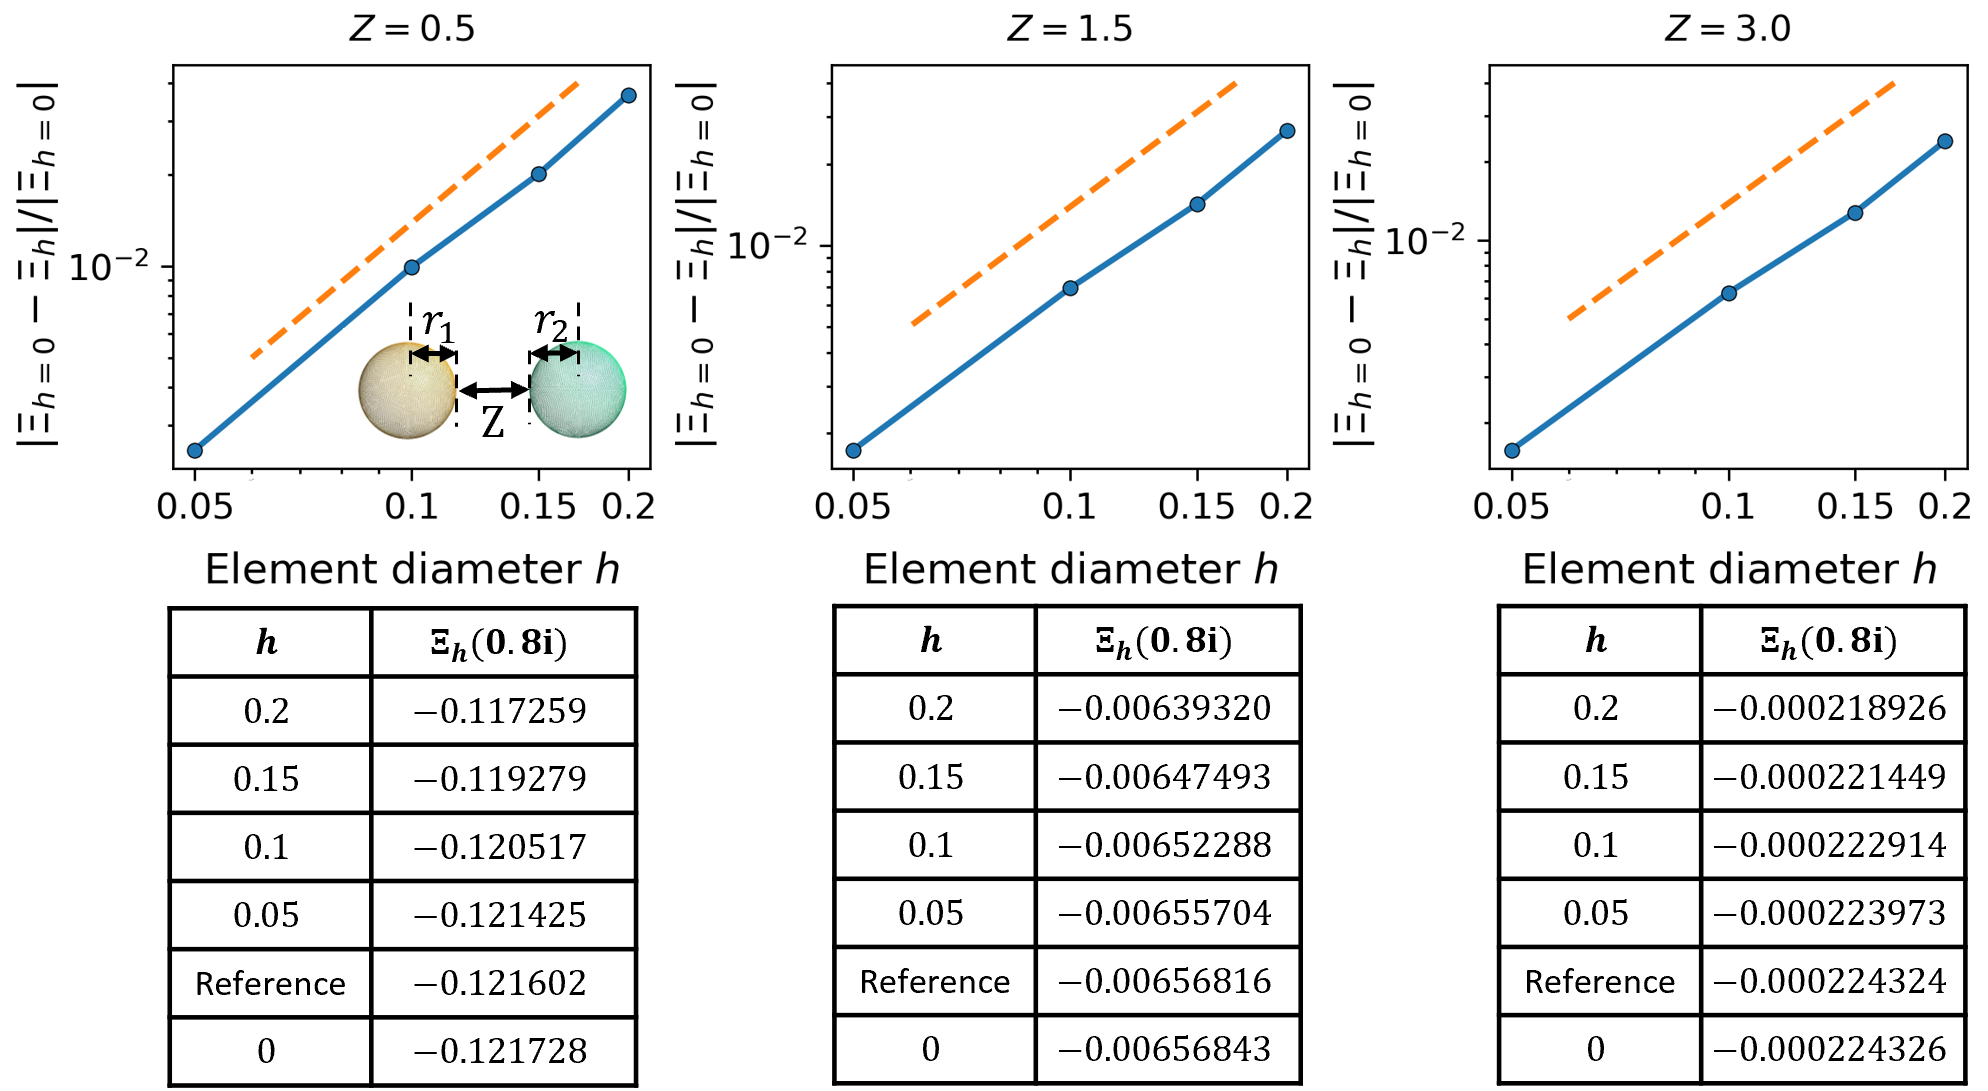
\includegraphics[width = \textwidth]{figures/Scalar_Xi_h_conv.png}
    \caption{$h$-convergence of $\Xi_{h}(\mathrm{i}k)$ to the extrapolation value $\Xi_{h = 0}(\mathrm{i}k)$ when $\mathrm{i}k = 0.8\mathrm{i}$. The provided reference values are accurate within $0.05\%$. The scatterers are two spheres with equal radii 1 and the distance between them is set as $Z = 0.5$, 1.5 and 3.0.
    The relative distance between $\Xi_{h}$ and $\Xi_{h = 0}$ decreases as we refine the mesh. The dashed line shows order 2 convergence. The tables list the values of $\Xi_{h}(0.8\mathrm{i})$ for $h = 0$, 0.05, 0.1, 0.15 and $0.2$, and the provided reference values.}
    \label{Scalar_Xi_h_conv}
\end{figure}

 Having shown the validation of the construction of $\Xi$, we are left with determining a proper upperbound for the Casimir integration. 
 The method for determining the upperbound of the integration is inspired by the asymptotic decay behavior of its integrand function.  
 By Figure \ref{Distinct:The integrand decays exponentially} and Figure \ref{The integrand decays exponentially}, the integrand value $\log\det\mathrm{V}(\mathrm{i}k)\tilde{\mathrm{V}}(\mathrm{i}k)^{-1}$ shares the same trend with $e^{-2Zk}$, this inspires us to apply the function $f(k) = Ce^{-2Zk}$ to fit the curve of the estimated integrand
 values. With the coefficient $C$ determined, one can estimate the absolute error for approximating the Casimir integral by computing:  
 \begin{align} \label{determine ub}
     \epsilon = \int_{\kappa}^{\infty}f(k)dk = \frac{Ce^{-2Z\kappa}}{2Z},
 \end{align}
 where $\kappa$ is the upperbound of the integration. Recall that we have changed the variable from $k$ to $y = e^{-k}$ when applying the normal trapezodial rule. This upperbound $\kappa$ corresponds to the lowerbound of $y$.
 

With the upperbound of the integration determined, one can start to estimate the Casimir energy between two spheres with radius $r_1 = r_2 = 1$ at the 
distance of $Z$ via the formula \eqref{KSSF and CasE} in two different refinement levels: $h_{\text{fine}} = 0.05$ 
($\text{dim}(\mathsf{V}_{\mathrm{i}k}) = 12603$) and $h_{\text{coarse}} = 0.1$ ($\text{dim}(\mathsf{V}_{\mathrm{i}k}) = 3192$).

Afterwards, the extrapolation result can be computed by these Casimir energy estimates. This result would be regarded as the extrapolation value of the 
Casimir energy, which would be used to compare with the 
estimates derived from the asymptotic series introduced below. 

According to \cite{emig2008casimir}, the Casimir energy between two spheres (with equal radii $r$) at asymptotically 
large separations can be obtained as a series in terms of the ratio of centre distance $L$ ($l = 2r + Z$) to sphere radius $R$:
\begin{align}\label{Asymptotic equal radii}
   \zeta_{\text{asy}} = -\frac{\hbar c}{\pi}\frac{1}{L}\sum_{n=0}^{\infty}b_{n}\left(\frac{r}{l}\right)^{n+2},
\end{align}
where the first six coefficients are 
$b_{0} = -1/4$, $b_{1} = -1/4$,  $b_{2} = -77/48$,  $b_{3} = -25/16$,  $b_{4} = -29837/2880$, $b_{5} = -6491/1152$. Figure 
\ref{Casimir energy between spheres with equal radii} shows the comparison between the Casimir energy computed from asymptotic series 
\eqref{Asymptotic equal radii} and the exact value evaluated through Richardson extrapolation and the reference value $\zeta_{\text{ref}}$ provided in \cite[Equation (64)]{kenneth2008casimir}. Here, we observe that the asymptotic value gradually 
approaches to the exact value as the distance $Z$ increases since the asymptotic expansion \eqref{Asymptotic equal radii} only works when the distance 
between two spheres is asymptotically large.

\begin{figure}[H]
    \centering
    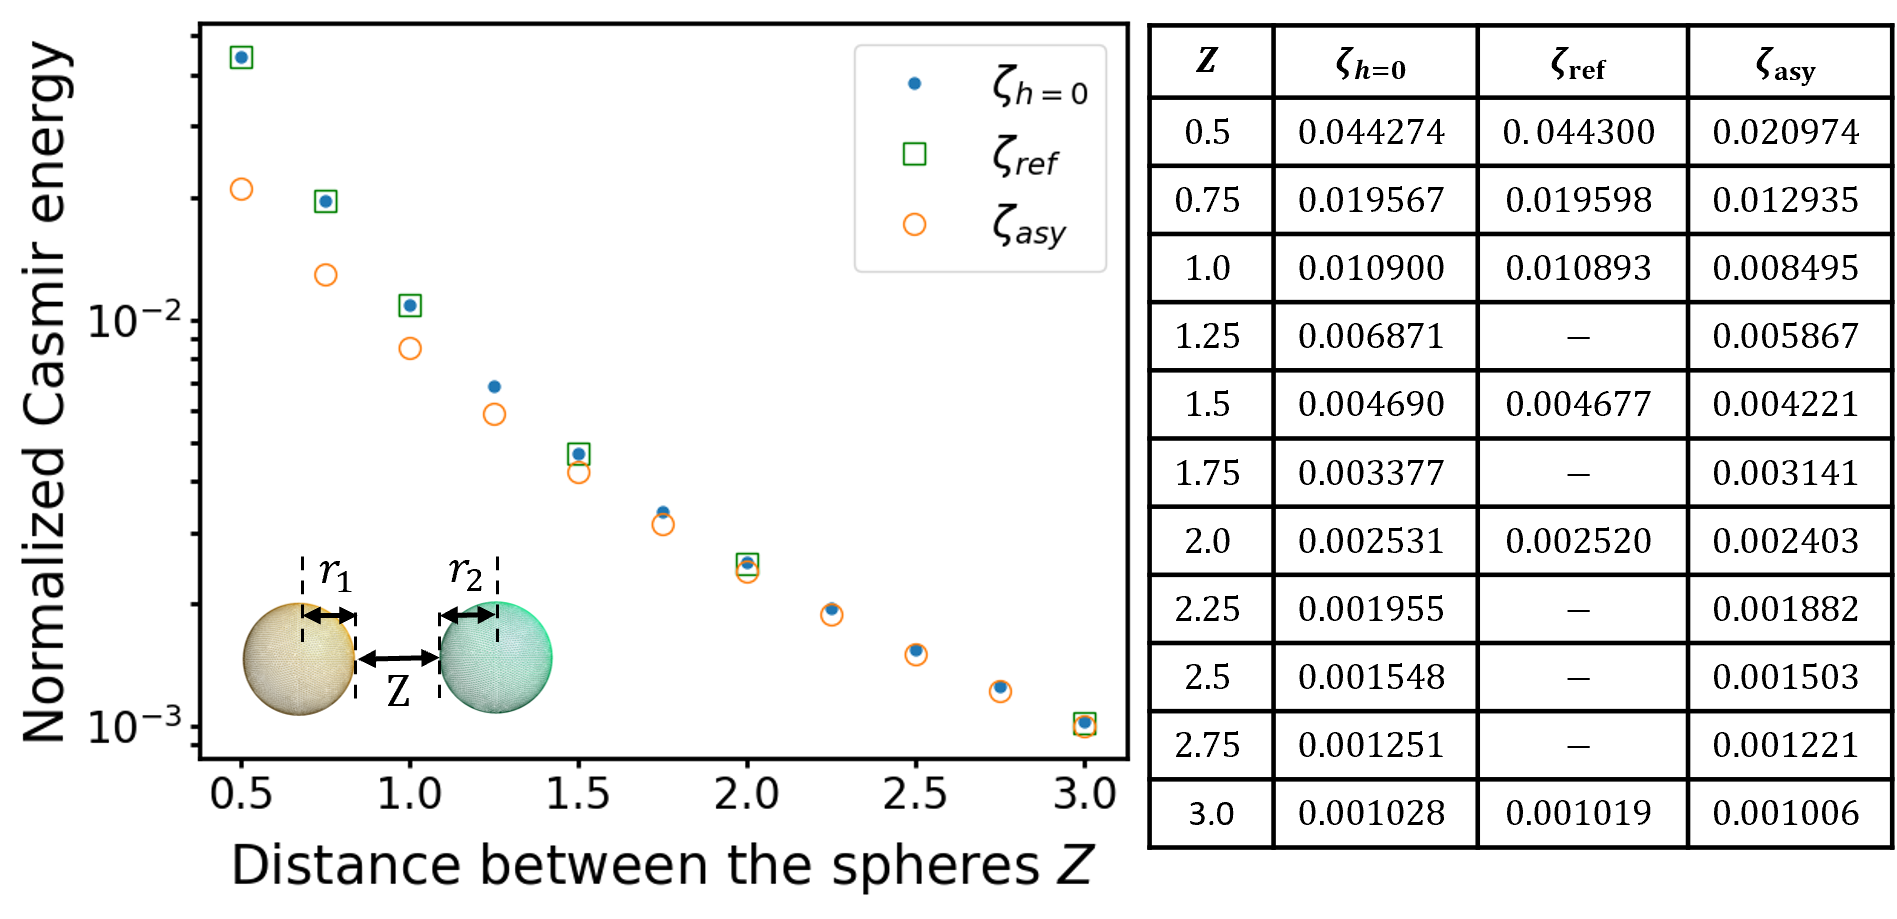
\includegraphics[width = \textwidth]{figures/Scalar_sp_equal_CasE.png}
    \caption[Caption for LOF]{{\color{gray}Left:} Negative normalized Casimir energy  \protect\footnotemark computed by the extrapolation (blue circle), asymptotic series (orange hollow circle) in two spheres with equal radii's case. The radius is $r_{1} = r_{2} = 1$ and the distance $Z$ 
    ranges from 0.5 to 3.0. The green hollow square represents the data of \cite{kenneth2008casimir}. {\color{gray}Right:} The table lists all the relevant data values in the figure.}
    \label{Casimir energy between spheres with equal radii}
\end{figure}
\footnotetext{The negative normalized Casimir energy is $-\mathcal{E}/\hbar c$, for $\mathcal{E}$ defined in \eqref{KSSF and CasE}.}

\begin{figure}[H]
    \centering
    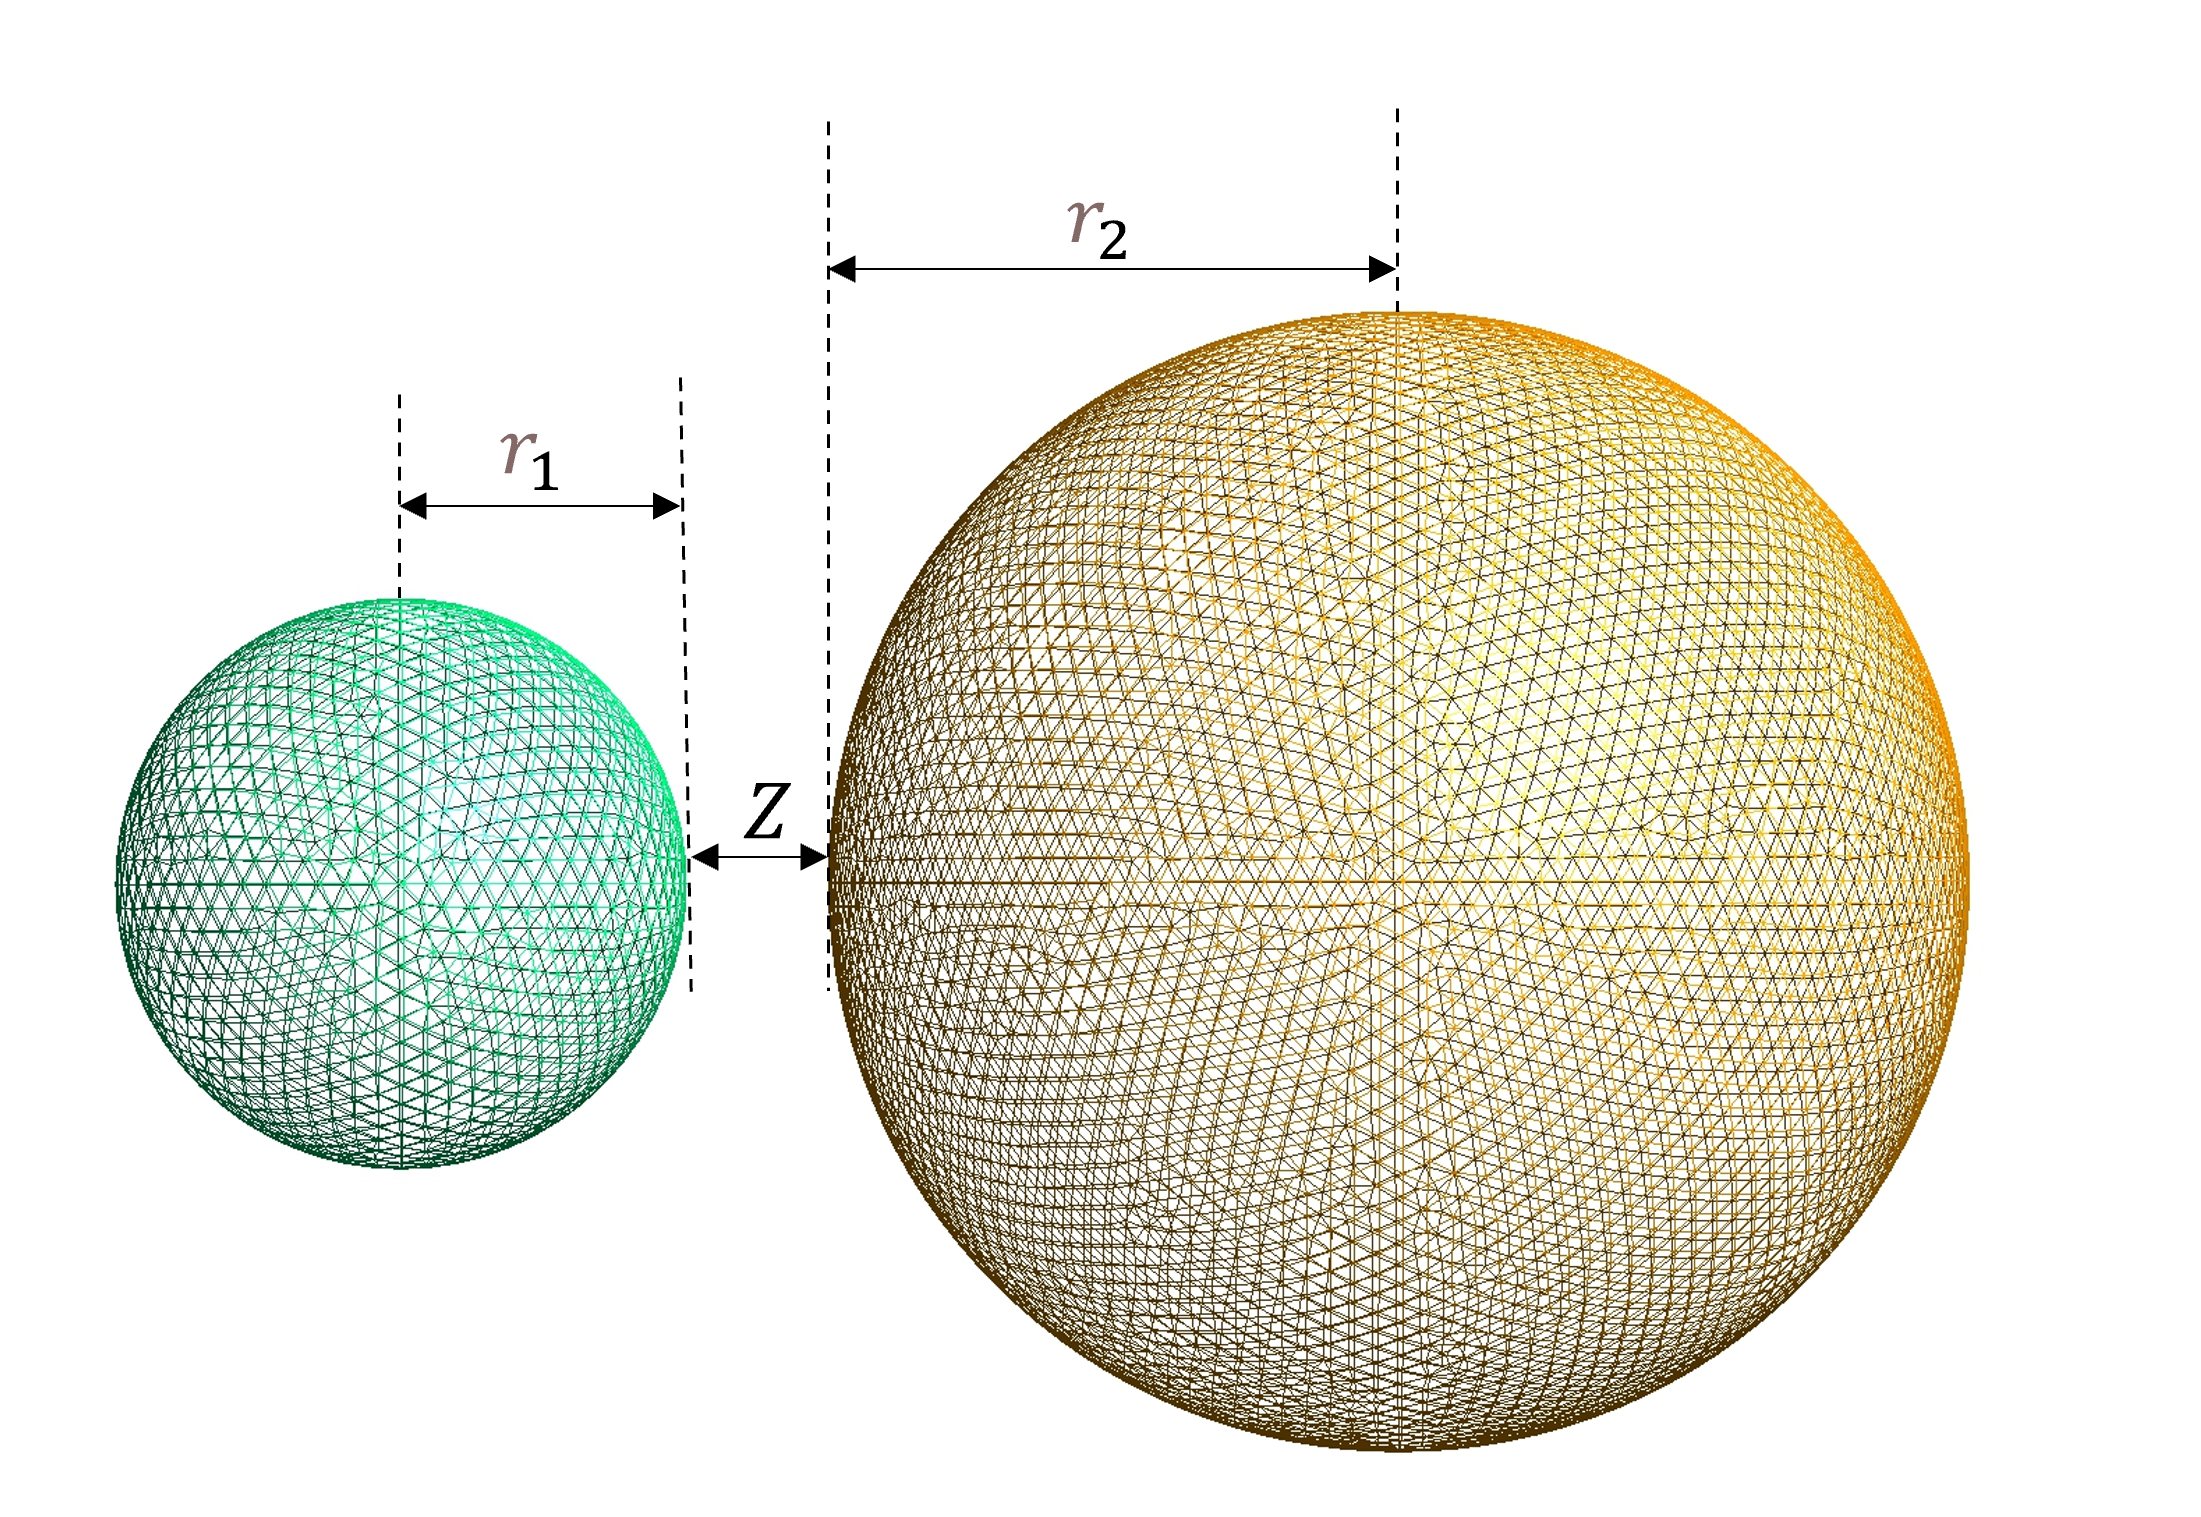
\includegraphics[scale = 0.5]{figures/Sphere_unequal_radii.png}
    \caption{Two spheres with unequal radii $r_{1} = 0.5$ and $r_{2} = 1$ and $Z$ is the minimal distance between them.\\
    \hspace*{1.5cm}$h_{\text{coarse}} = 0.1$: $\text{dim}(\mathrm{V}_{\mathrm{i}k}) = 2023$,  N\textsuperscript{\underline{o}} of elements on both grids $ = 4038$;\\
    \hspace*{1.5cm}$h_{\text{fine}} = 0.05$: $\text{dim}(\mathrm{V}_{\mathrm{i}k}) = 7891$,  N\textsuperscript{\underline{o}} of elements on both grids $ = 15774$}
    \label{Two spheres with unequal radii}
\end{figure}

Now, let us consider the case when two spheres have different radii $r_{1}$, $r_{2}$ (see Figure \ref{Two spheres with unequal radii}). 

In this case, one can still determine the upperbound of the integration by fitting the integrand function curve and considering the error tolerance.
Afterwards, we would like to compare the extrapolation value of the Casimir energy computed through the Richardson extrapolation with the asymptotic expansion. By denoting the centre distance as
$l = r_{1} + r_{2} + Z$, the asymptotic series of the Casimir energy between these two spheres is written by
\begin{align}\label{Asymptotic unequal radii}
    \zeta_{\text{asy}} = -\frac{\hbar c}{\pi}\frac{1}{l}\sum_{n=0}^{\infty}\tilde{b}_{n}(\eta)\left(\frac{r_{1}}{L}\right)^{n+2},
\end{align}
where the coefficients $\{\tilde{b}_{n}\}$ depend on the parameter $\eta = r_{2}/r_{1}$ and the first six coefficients are
\begin{align*}
    \tilde{b}_{0} &= -\frac{\eta}{4}, \ \ \ \ \ \tilde{b}_{1} = -\frac{\eta + \eta^{2}}{8}, \ \ \ \ \  \tilde{b}_{2} = -\frac{34(\eta+\eta^{3})+ 9\eta^{2}}{48}, \ \ \ \ \ \tilde{b}_{3} = -\frac{2(\eta+\eta^{4}) + 23(\eta^{2} + \eta^{3})}{32}, \\ 
    \tilde{b}_{4} &= -\frac{8352(\eta + \eta^{5})+ 1995(\eta^{2} + \eta^{4}) + 38980\eta^{3}}{5760}, \ \ \ \ \ \tilde{b}_{5} = -\frac{-1344(\eta+\eta^{6}) + 5478(\eta^{2} + \eta^{5})+2357(\eta^{3} + \eta^{4})}{2304}.
\end{align*}

In the following experiment, the radii of the spheres shown in Figure \ref{Two spheres with unequal radii} are set as $r_{1} = 0.5$ and $ r_{2} = 1$. 
As in the previous example, the exact value of the Casimir energy is computed through the Richardson extrapolation and the coarse and fine grid size are $h_{\text{fine}} = 0.05$ ($\text{dim}(\mathsf{V}_{\mathrm{i}k}) = 7893)$ and 
$h_{\text{coarse}} = 0.1$ ($\text{dim}(\mathsf{V}_{\mathrm{i}k}) = 2023)$, separately. 

In this case, the asymptotic value of the Casimir 
energy was estimated by the series \eqref{Asymptotic unequal radii} and the comparison between the extrapolation value and asymptotic one is shown in Figure 
\ref{Casimir energy between spheres with unequal radii}. Again, one can notice that when the distance between two spheres decreases, the asymptotic value gets 
close to the extrapolation one.
\begin{figure}[H]
    \centering
    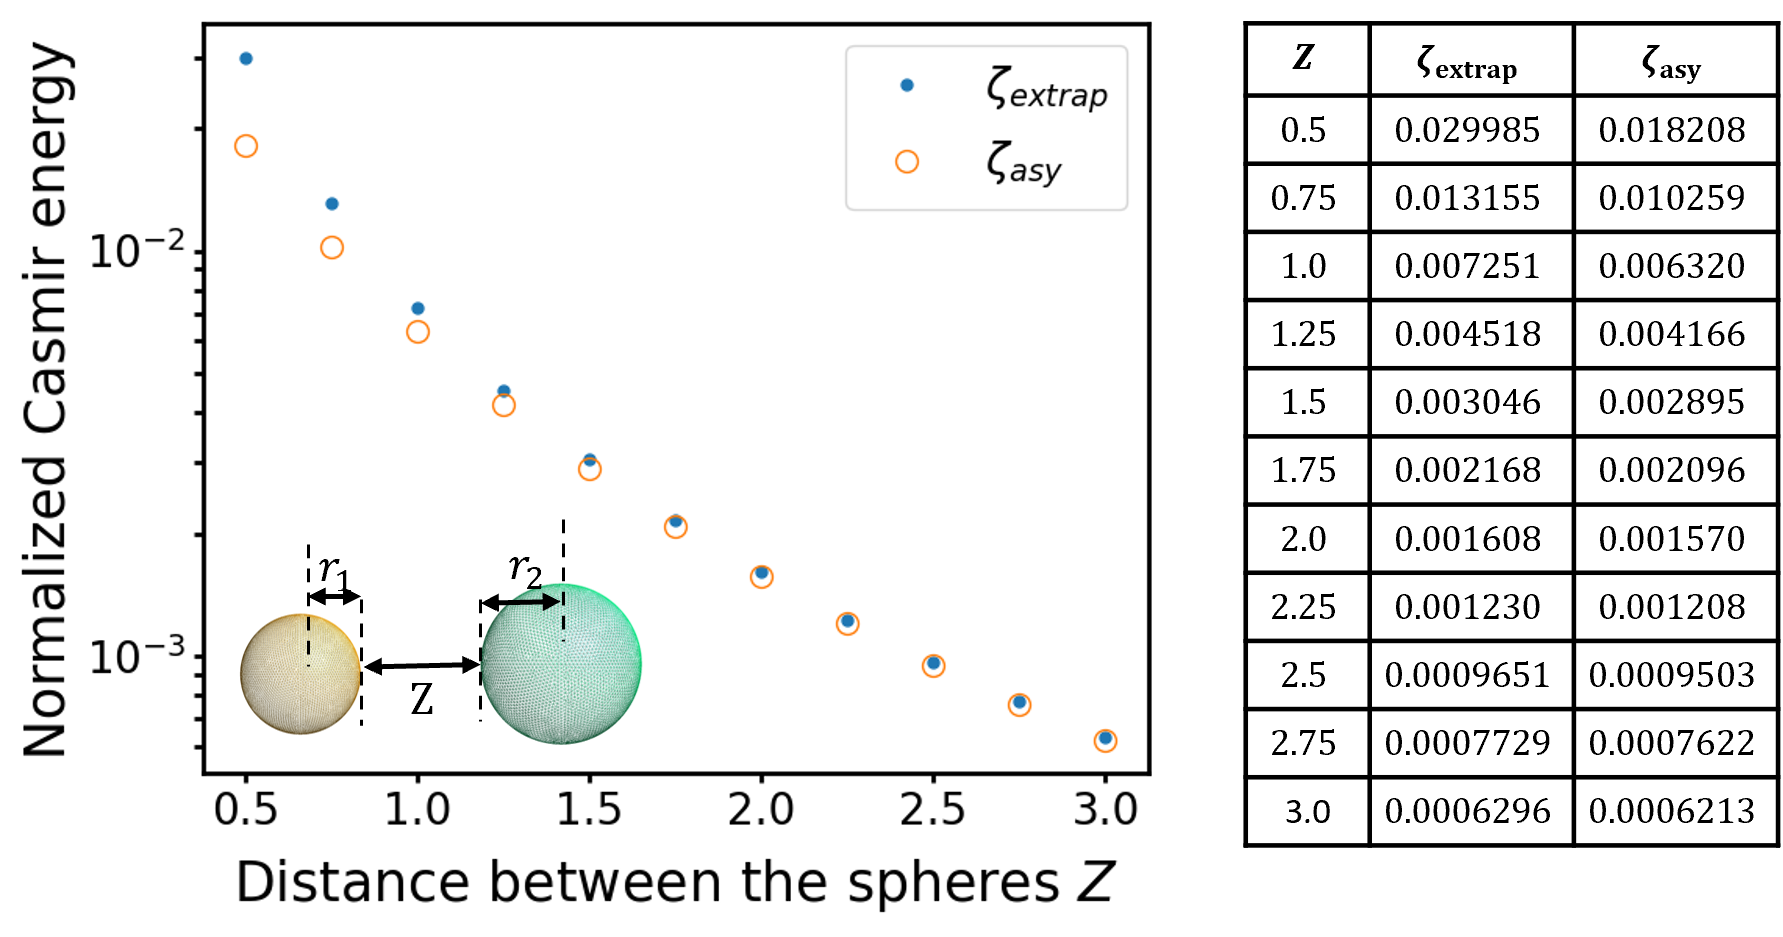
\includegraphics[width = \textwidth]{figures/Spheres_unequal_CasE.png}
    \caption{Negative normalized Casimir energy in two spheres with unequal radii's case. The radius is $R = 1$ and the distance $Z$ 
    ranges from 0.5 to 3.0. The exact value of the (negative normalized) Casimir energy has been written 
    beside the data point, which is round up to 4 significant digits.}
    \label{Casimir energy between spheres with unequal radii}
\end{figure}

After showing the validation of the numerical framework for computing the Casmir energy, we would like to end this section with computing the negative normalized Casimir energy between one torus and one sphere. For the torus, it is centering at the origin and the distance from the center of the tube to the center of the torus is $l_1 = 2$ and the radius of the tube is $l_2 = 0.5$; for the sphere, 
it has radius $r = 1$ and its center is always on the $z$-axis (see Figure \ref{fig:Torus_sphere_CasE} (Right)). By  Figure \ref{fig:Torus_sphere_CasE} (Left), one can see that when the sphere and the torus share the same center, the negative normalized Casimir energy has the largest magnitude. This means if one put this sphere at the origin in the beginning, this attractive effect will make the torus hold the sphere stationary. 


\begin{figure}[H]
\centering
\begin{minipage}{.65\textwidth}
  \centering
  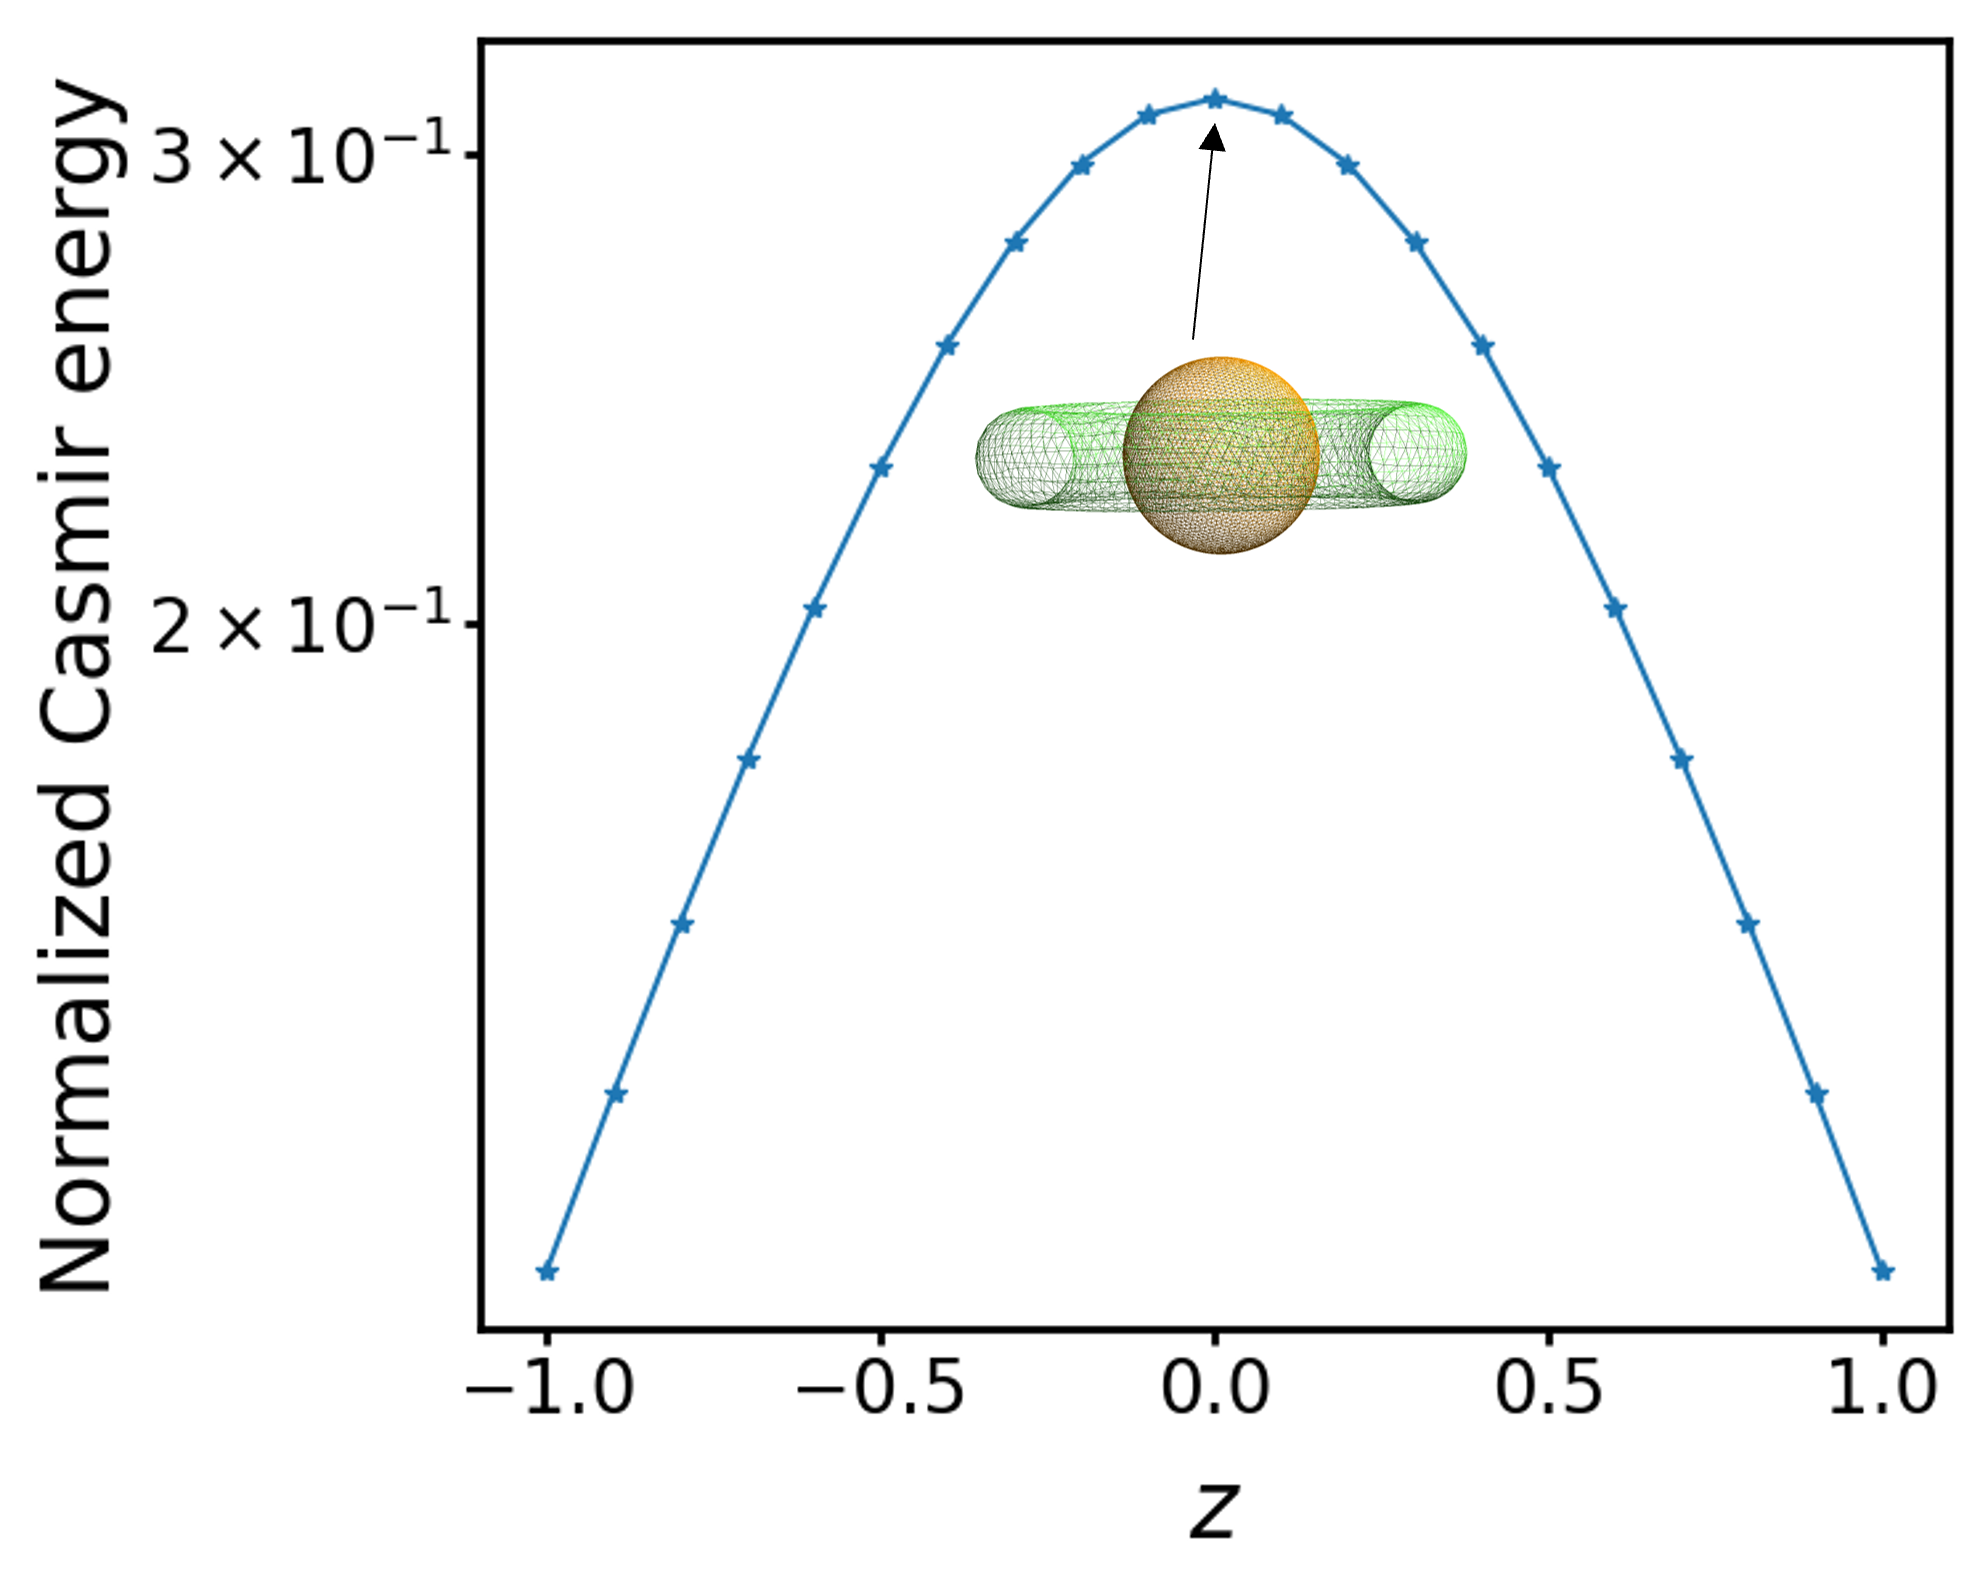
\includegraphics[width=\textwidth]{figures/Torus_sphere_CasE.png}
\end{minipage}%
\begin{minipage}{.35\textwidth}
  \centering
  \vspace*{-0.6cm}
  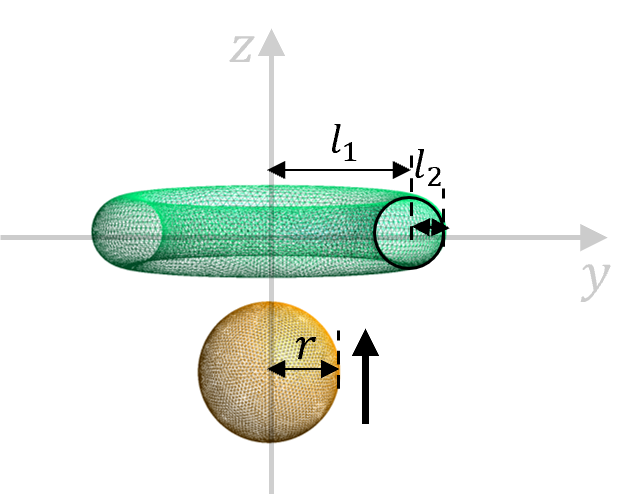
\includegraphics[width=\textwidth]{figures/Sphere_torus.png}
%   \caption{A subfigure}
%   \label{fig:Sphere_torus}
\end{minipage}
\caption{Negative normalized Casimir energy between a torus and a sphere when the sphere moves along the $z$-axis. The parameters of the torus are $l_1 = 2$, $l_2 = 0.5$ and the radius of the sphere is $r = 1$.}
\label{fig:Torus_sphere_CasE}
\end{figure}


\subsection{Realistic objects case}
In this part, the Casimir energy between the objects with special shapes such as the menger sponges, ice crystals and ellipsoids will be computed 
through the Richardson extrapolation mentioned in the beginning of this section and the values labelled in the following figures are accurate within three significant digits. 
Note that the matrix size of the involved matrix in each example has been stated in the figures.

Figure \ref{Menger sponges} plots the menger sponges in different levels $(0, 1 $ and $ 2)$ and the length of these sponges is always 1. Afterwards, the Casimir 
energy between two menger sponges in the same level are listed in Table \ref{Negative normalized Casimir energy in two menger sponges' case}. 
In addition, inside the extrapolation process, when $h_{\text{fine}} = 0.05$, the $\text{dim}(\mathsf{V}_{\mathrm{i}k}) = 5664$, 8510 and 27136 and 
when $h_{\text{coarse}} = 0.1$, the $\text{dim}(\mathsf{V}_{\mathrm{i}k}) = 1456$, 3092 and 14464 in different level (0, 1 and 2) cases, separately. 
By comparing the data 
point in this table, it is easy to find that the Casimir energy decreases as the number of the iteration increases since the cross-sectional 
area gets smaller.

\begin{figure}[H]
    \centering
    \captionsetup[subfigure]{justification=centering}
    \subfloat[Level 0 \\ $h_{\text{coarse}} = 0.1$: $\text{dim}(\mathsf{V}_{\mathrm{i}k}) = 1456$,  N\textsuperscript{\underline{o}} of elements on both grids $ = 2904$
    \\ $h_{\text{fine}} = 0.05$: $\text{dim}(\mathsf{V}_{\mathrm{i}k}) = 5664$,  N\textsuperscript{\underline{o}} of elements on both grids $ = 11120$]{{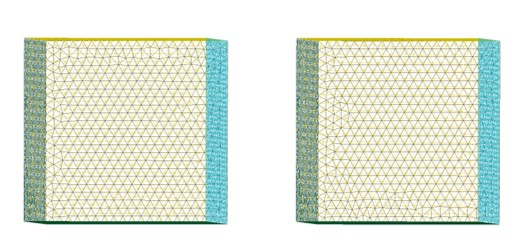
\includegraphics[scale = 0.5]{figures/merger_sponge_level0.jpg} }}
    \qquad
    \subfloat[Level 1 \\ $h_{\text{coarse}} = 0.1$: $\text{dim}(\mathsf{V}_{\mathrm{i}k}) = 3092$,  N\textsuperscript{\underline{o}} of elements on both grids $ = 6216$
    \\ $h_{\text{fine}} = 0.05$: $\text{dim}(\mathsf{V}_{\mathrm{i}k}) = 8510$,  N\textsuperscript{\underline{o}} of elements on both grids $ = 17052$]{{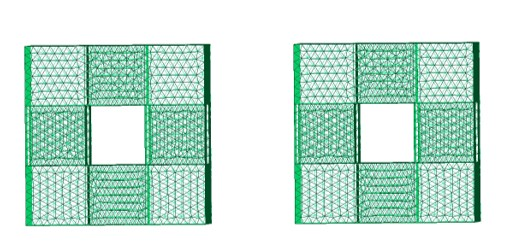
\includegraphics[width=0.4\textwidth]{figures/merger_sponge_level1.jpg} }}
    \qquad
    \subfloat[Level 2 \\ $h_{\text{coarse}} = 0.1$: $\text{dim}(\mathsf{V}_{\mathrm{i}k}) = 14464$,  N\textsuperscript{\underline{o}} of elements on both grids $ = 29568$
    \\ $h_{\text{fine}} = 0.05$: $\text{dim}(\mathsf{V}_{\mathrm{i}k}) = 27136$,  N\textsuperscript{\underline{o}} of elements on both grids $ = 54912$]{{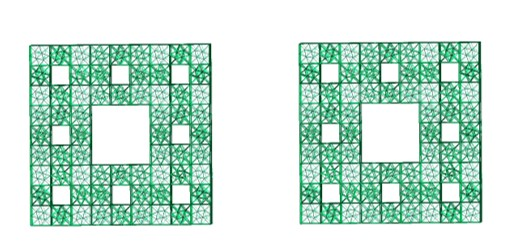
\includegraphics[width=0.5\textwidth]{figures/merger_sponge_level2.jpg} }}
    \caption{Menger sponges in different levels. The length of each sponge is 1.}
    \label{Menger sponges}
\end{figure}

\begin{table}[H]
    \centering
    \begin{tabular}{ |P{2cm}||p{2cm}|p{2cm}|p{2cm}|  }
        \hline
        \multicolumn{4}{|c|}{Negative normalized Casimir energy in two menger sponges' case} \\
        \hline
        Distance & Level 0 & Level 1 & Level 2\\
        \hline
        0.5   & 0.08350    & 0.08229     & 0.08112\\
        0.75  & 0.02737    & 0.02688     & 0.02670\\
        1.0   & 0.01305    & 0.01288     & 0.01282\\
        1.25  & 0.007357   & 0.007283    & 0.007252\\
        1.5   & 0.004607   & 0.004568    & 0.004551\\
        1.75  & 0.003099   & 0.003076    & 0.003065\\
        2.0   & 0.002195   & 0.002181    & 0.002174\\
        2.25  & 0.001618   & 0.001608    & 0.001603\\
        2.5   & 0.001230   & 0.001223    & 0.001220\\
        2.75  & 0.0009593  & 0.0009541   & 0.0009514\\
        3.0   & 0.0007638  & 0.0007598   & 0.0007577\\
        \hline
       \end{tabular}
       \caption{\label{Negative normalized Casimir energy in two menger sponges' case} Negative normalized Casimir energy in two menger sponges' case}
    \end{table}

\begin{figure}[H]
    \centering
    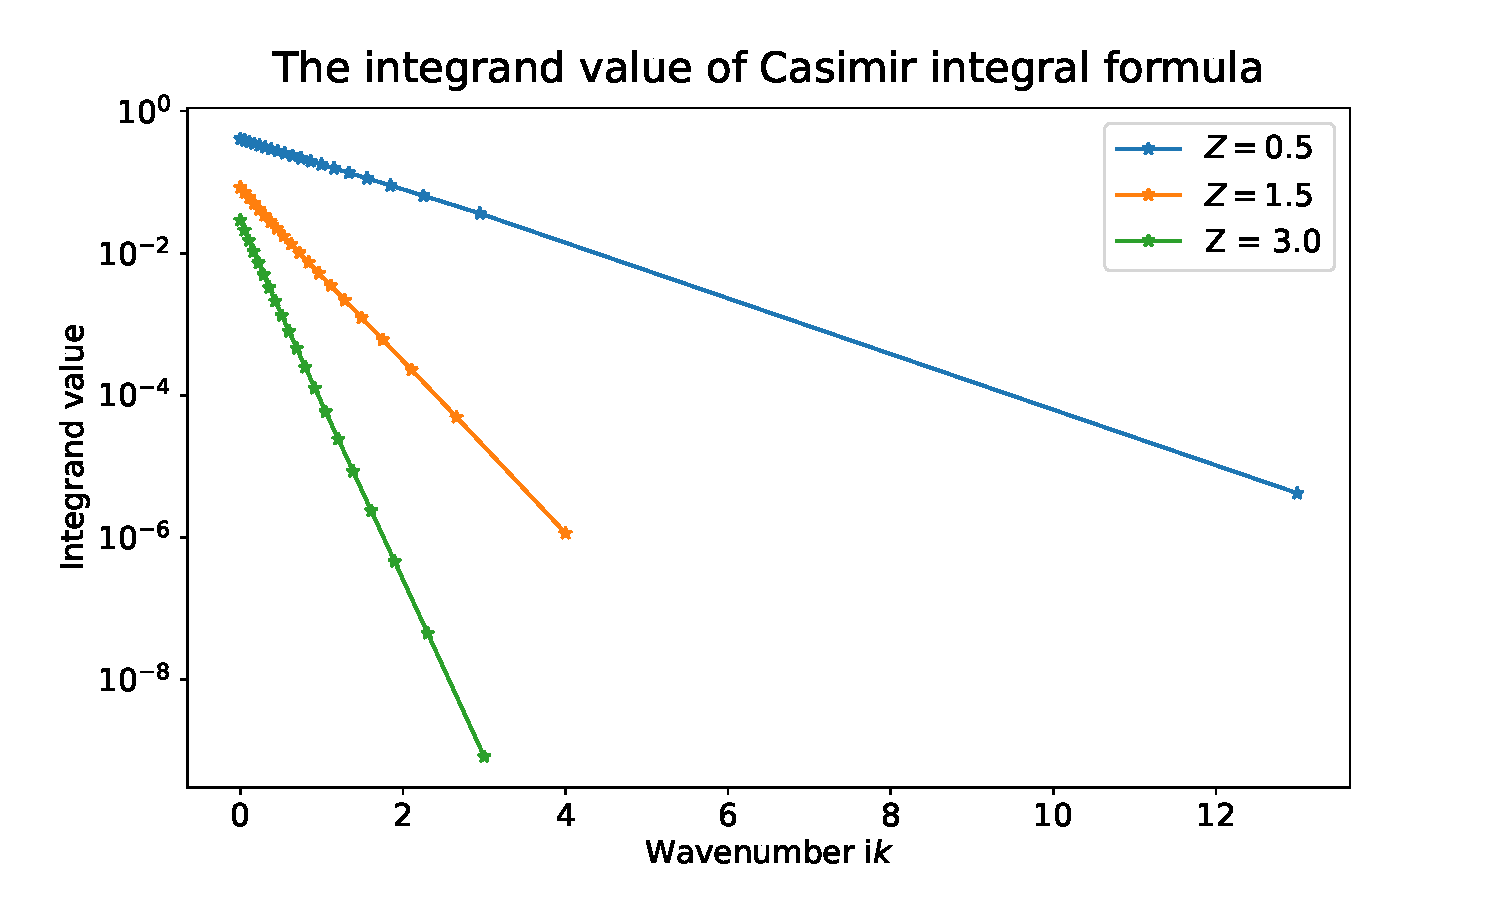
\includegraphics[scale = 1]{figures/level1_integrand_Value.png}
    \caption{The integrand of the Casimir energy between two menger sponges in Level 1 with distance $Z = 0.5$, 1.5 and 3.0.}
    \end{figure}

\begin{figure}[H]
        \centering
        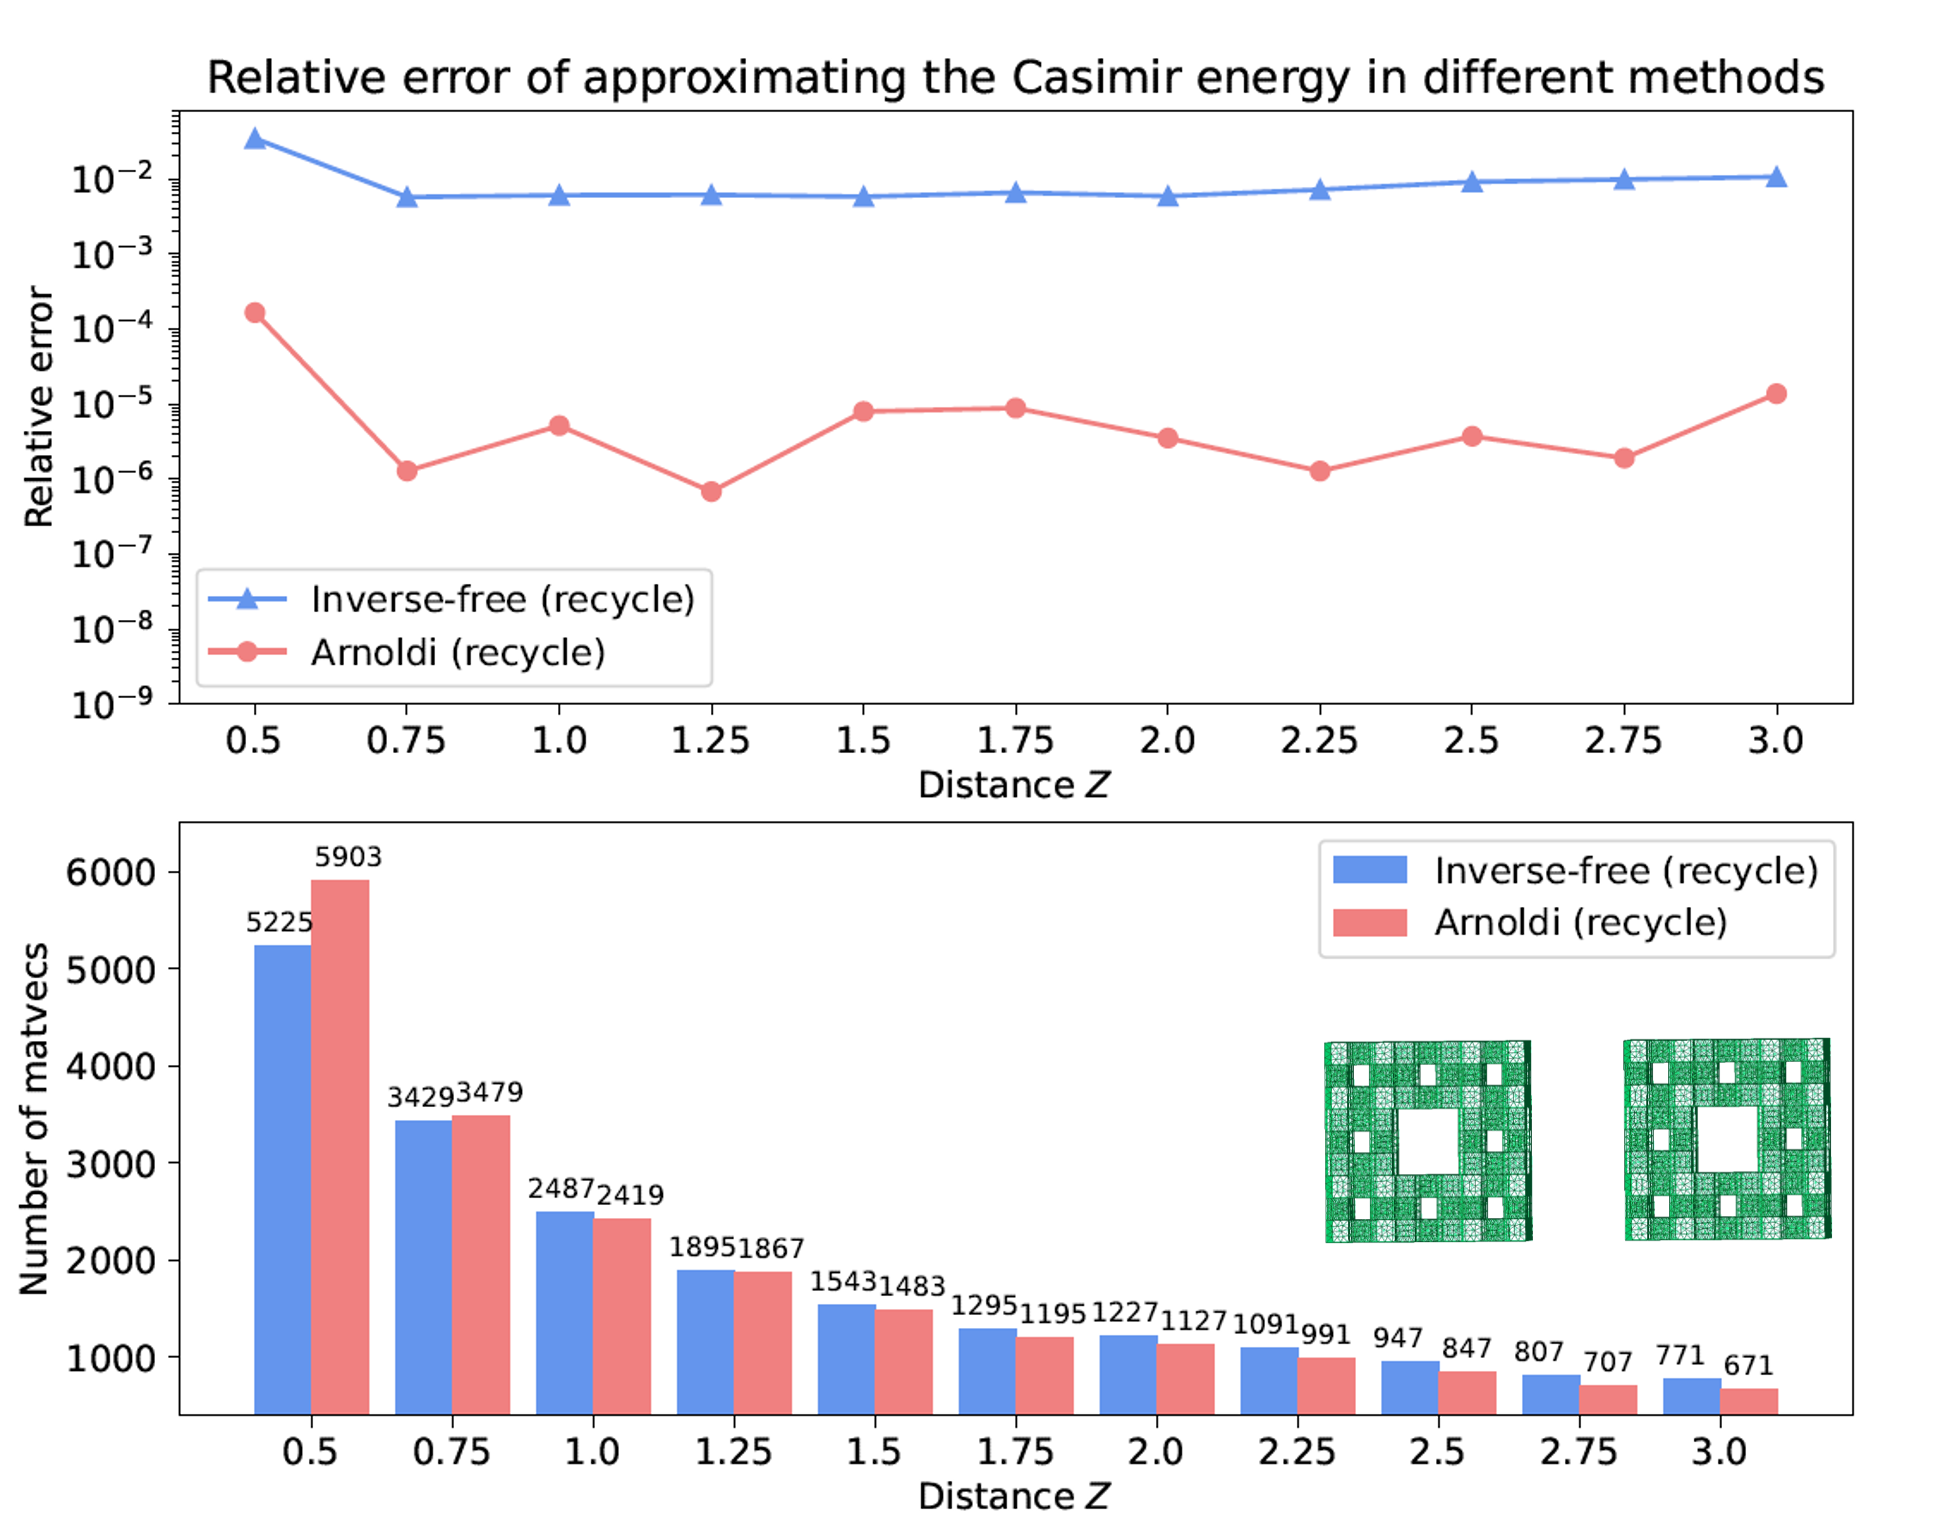
\includegraphics[width = \textwidth]{figures/level2_rel_err.png}
        \caption{Menger sponges in Level 2's case: relative distance between the reference value (computed by Richardson extrapolation) with the estimates evaluated from the standard Arnoldi 
        method with subspace recycled (solid red circles) and inverse-free Krylov subspace method 
        with subspace recycled (solid blue triangles). The dimension of the Krylov subspace is $m = 100$. The recycled eigenvectors have the corresponding eigenvalue 
        whose logarithm is larger than $10^{-5}$.}
\end{figure}


%==========================================================================================
In the next example, the scatterers are ice crystals with different number of branches ranging from 2 to 6 (see Figure \ref{Ice crystals with different number of branches}).

\begin{figure}[H]
    \begin{subfigure}{0.3\linewidth}
        \centering
        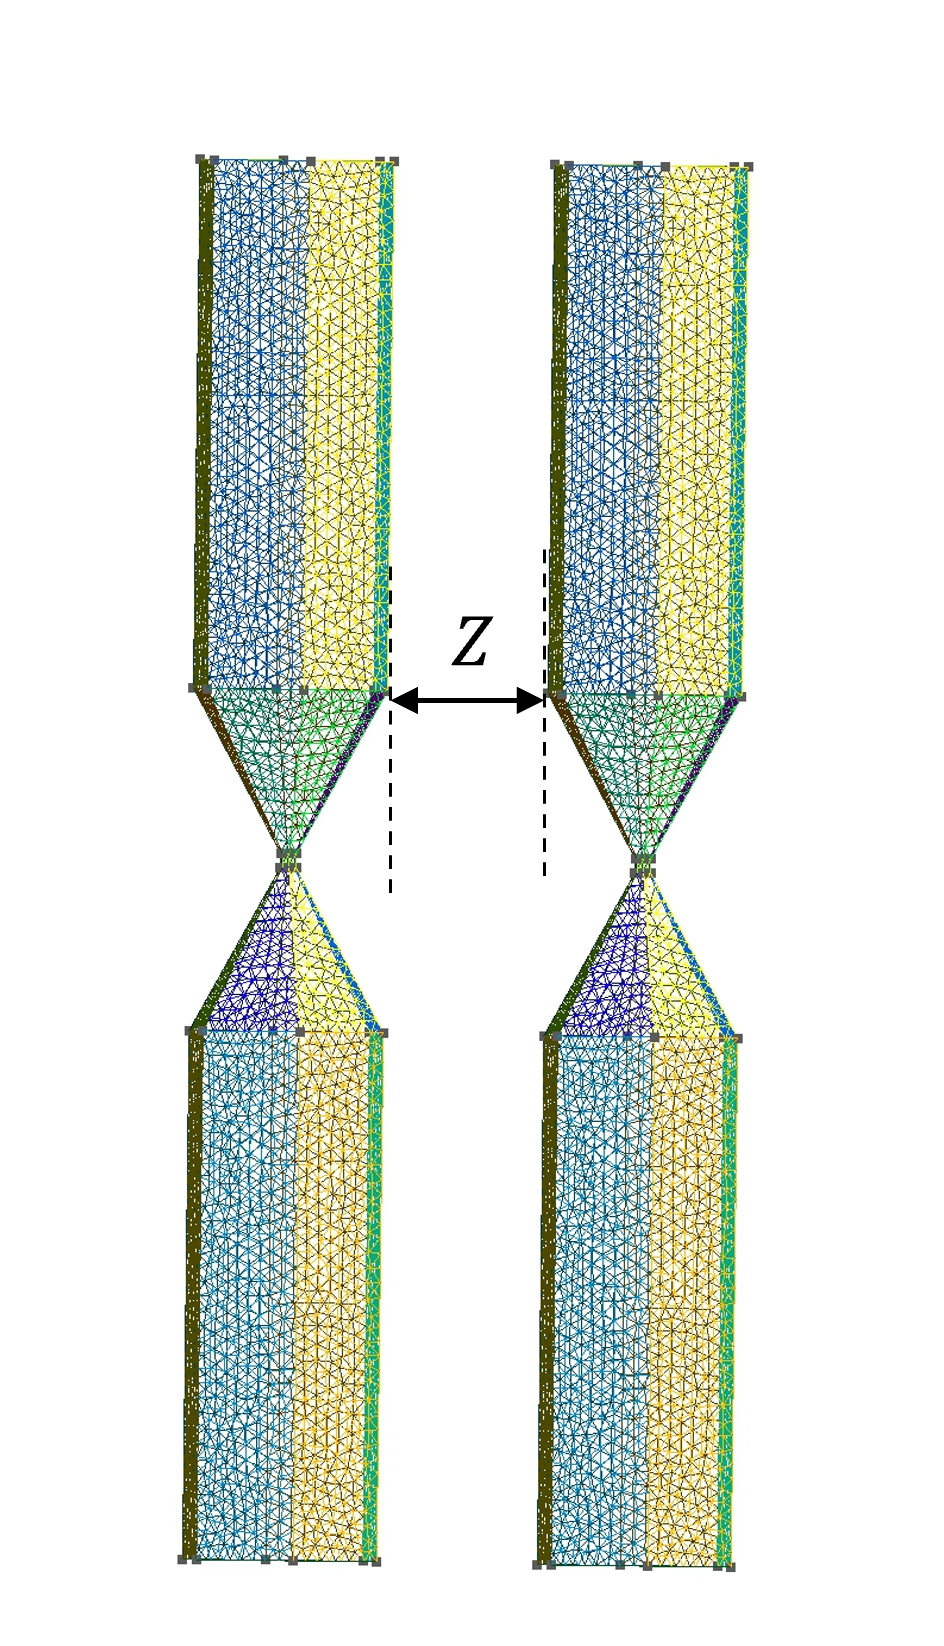
\includegraphics[scale = 0.4]{figures/2branches}
        \caption{Two branches: $\text{dim}(\mathsf{V}_{\mathrm{i}k}) = 8792$ \newline N\textsuperscript{\underline{o}} of elements on both grids $ = 17576$}
        \end{subfigure}
        \begin{subfigure}{0.3\linewidth}
            \centering
            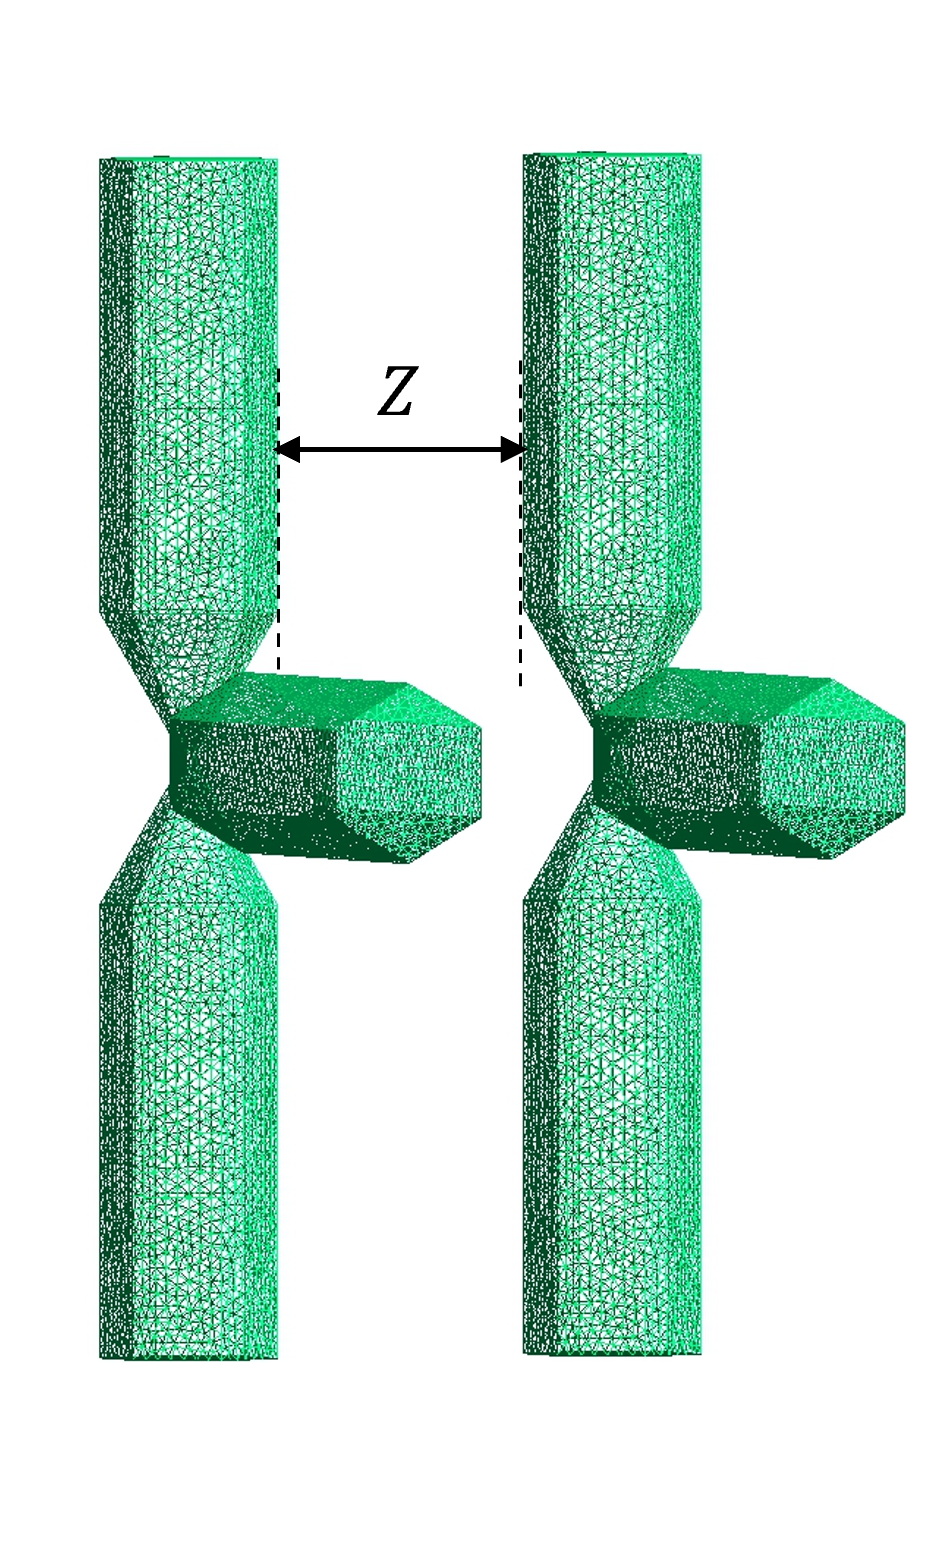
\includegraphics[scale = 0.4]{figures/3branches}
            \caption{Three branches: $\text{dim}(\mathsf{V}_{\mathrm{i}k}) = 13104$ \newline N\textsuperscript{\underline{o}} of elements on both grids $ = 26200$}
            \end{subfigure}
            \begin{subfigure}{0.3\linewidth}
                \centering
                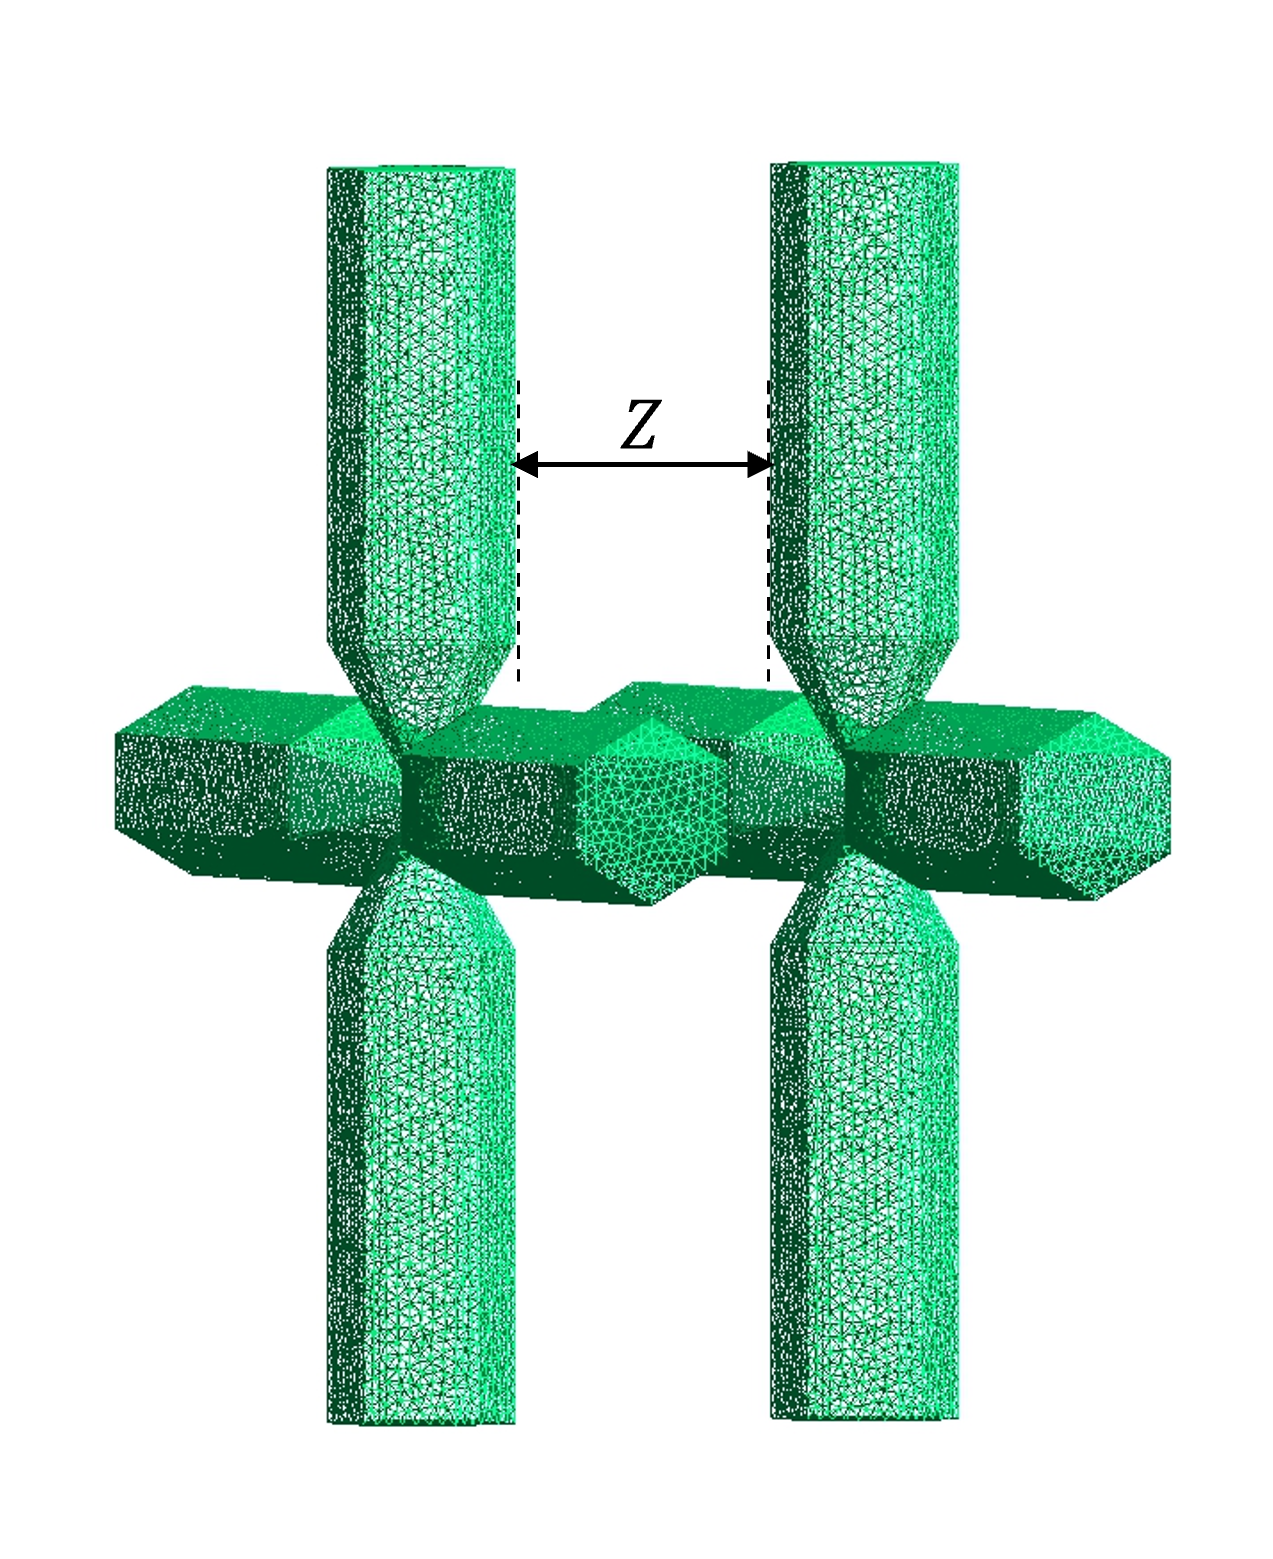
\includegraphics[scale = 0.4]{figures/4branches}
                \caption{Four branches: $\text{dim}(\mathsf{V}_{\mathrm{i}k}) = 17554$ \newline N\textsuperscript{\underline{o}} of elements on both grids $ = 35100$}
                \end{subfigure}\\[1ex]
    %\begin{subfigure}{.5\linewidth}
    \centering
    \captionsetup[subfigure]{oneside,margin={0.4cm,0cm}}
    \subfloat[Five branches: $\text{dim}(\mathsf{V}_{\mathrm{i}k}) = 21950$ \newline N\textsuperscript{\underline{o}} of elements on both grids $ = 43900$]{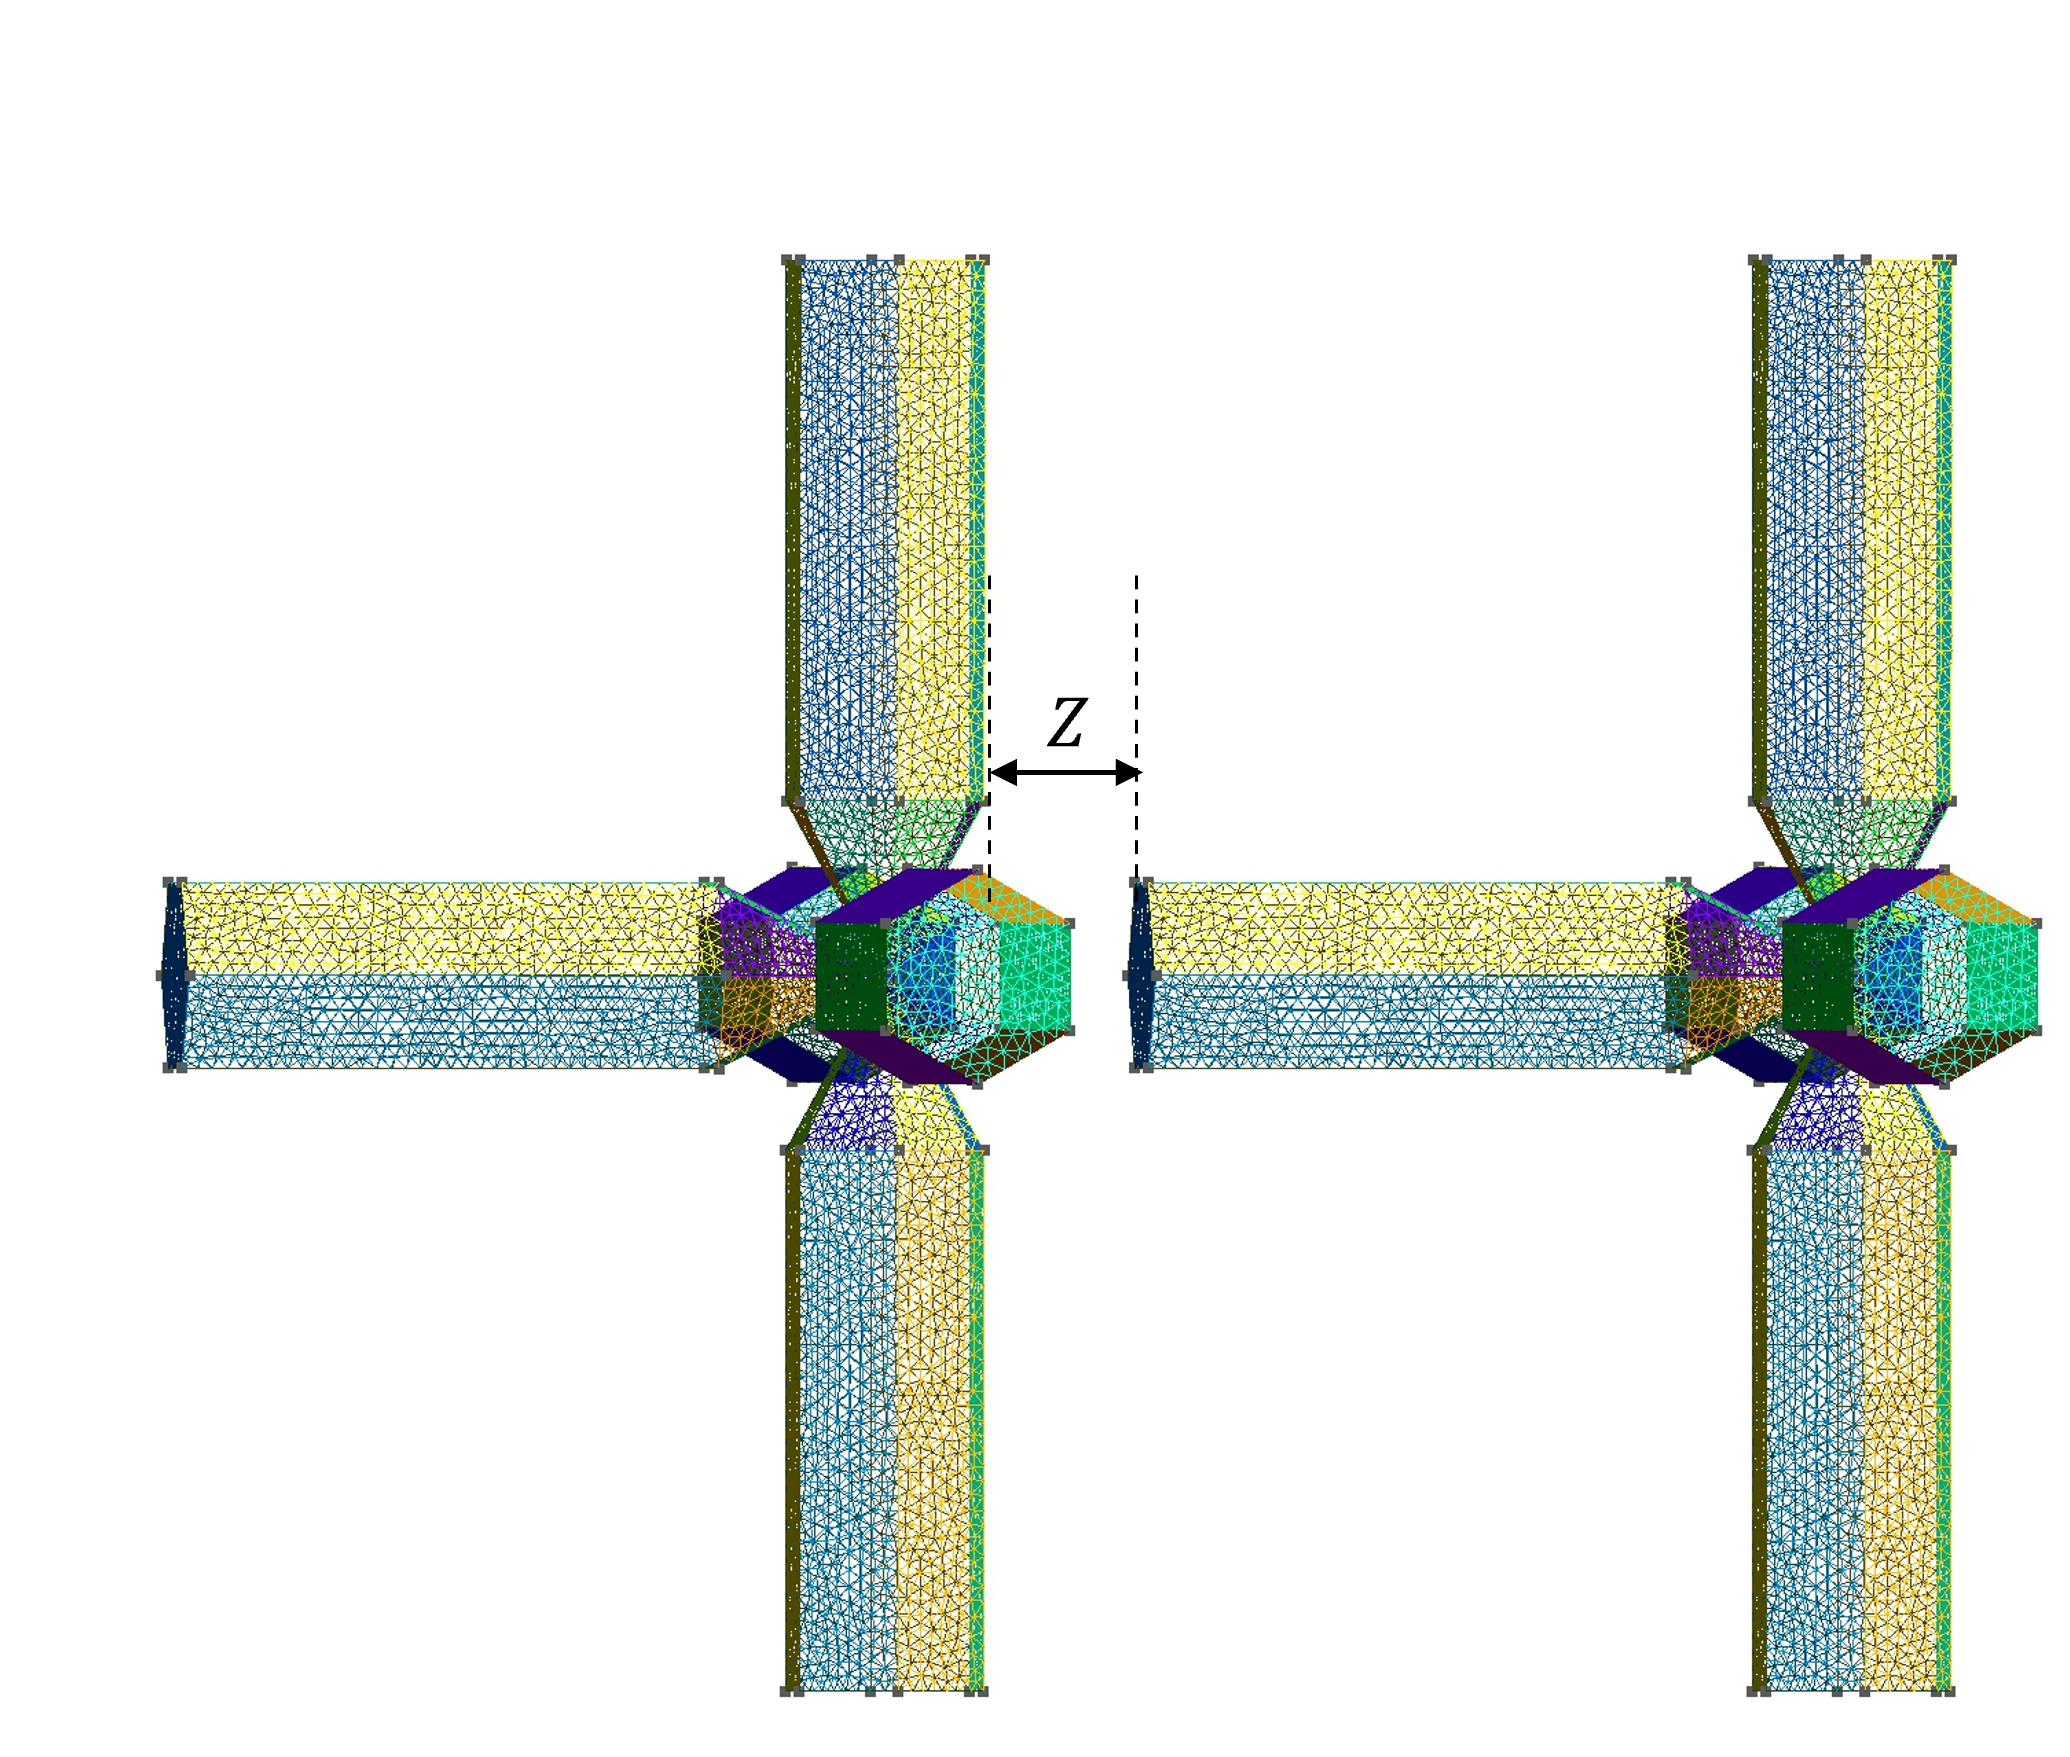
\includegraphics[scale=0.4]{figures/5branches}}
    %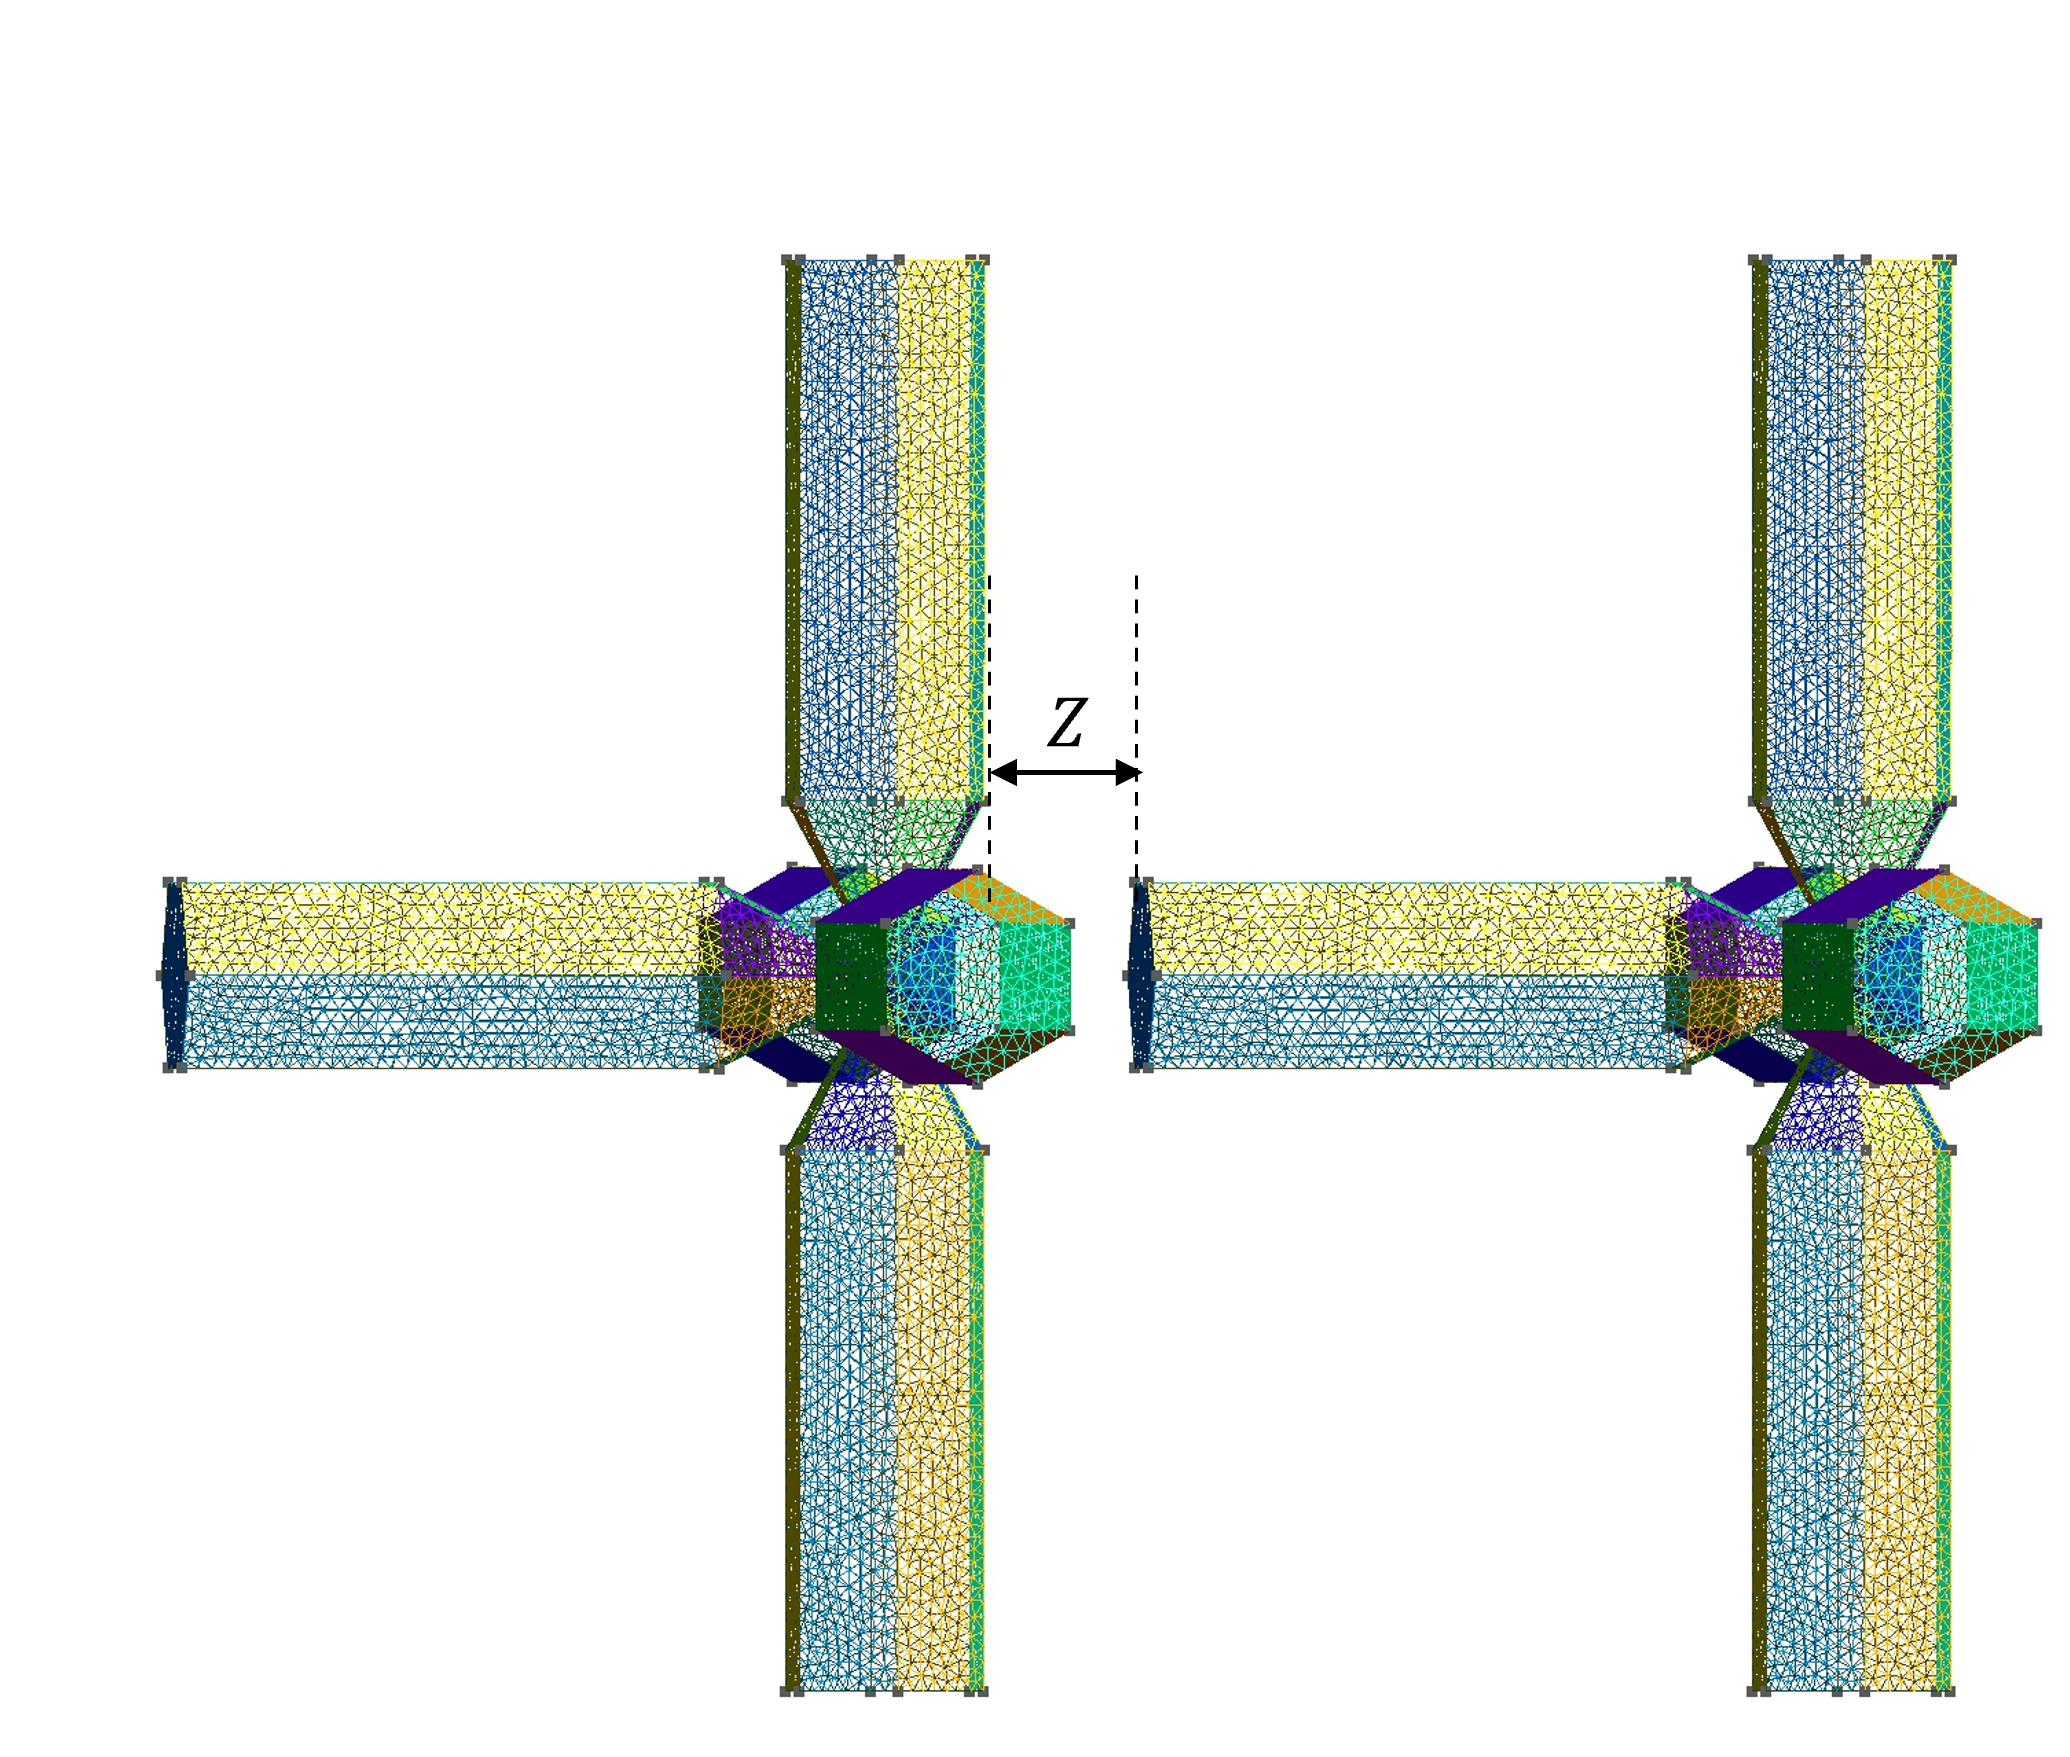
\includegraphics[scale = 0.4]{figures/5branches}
    %\caption{Five branches: $\text{dim}(\mathsf{V}_{\mathrm{i}k}) = 21950$ \newline N\textsuperscript{\underline{o}} of elements on both grids $ = 43900$}
    %\end{subfigure}%
    %\begin{subfigure}{.5\linewidth}
    \centering
    %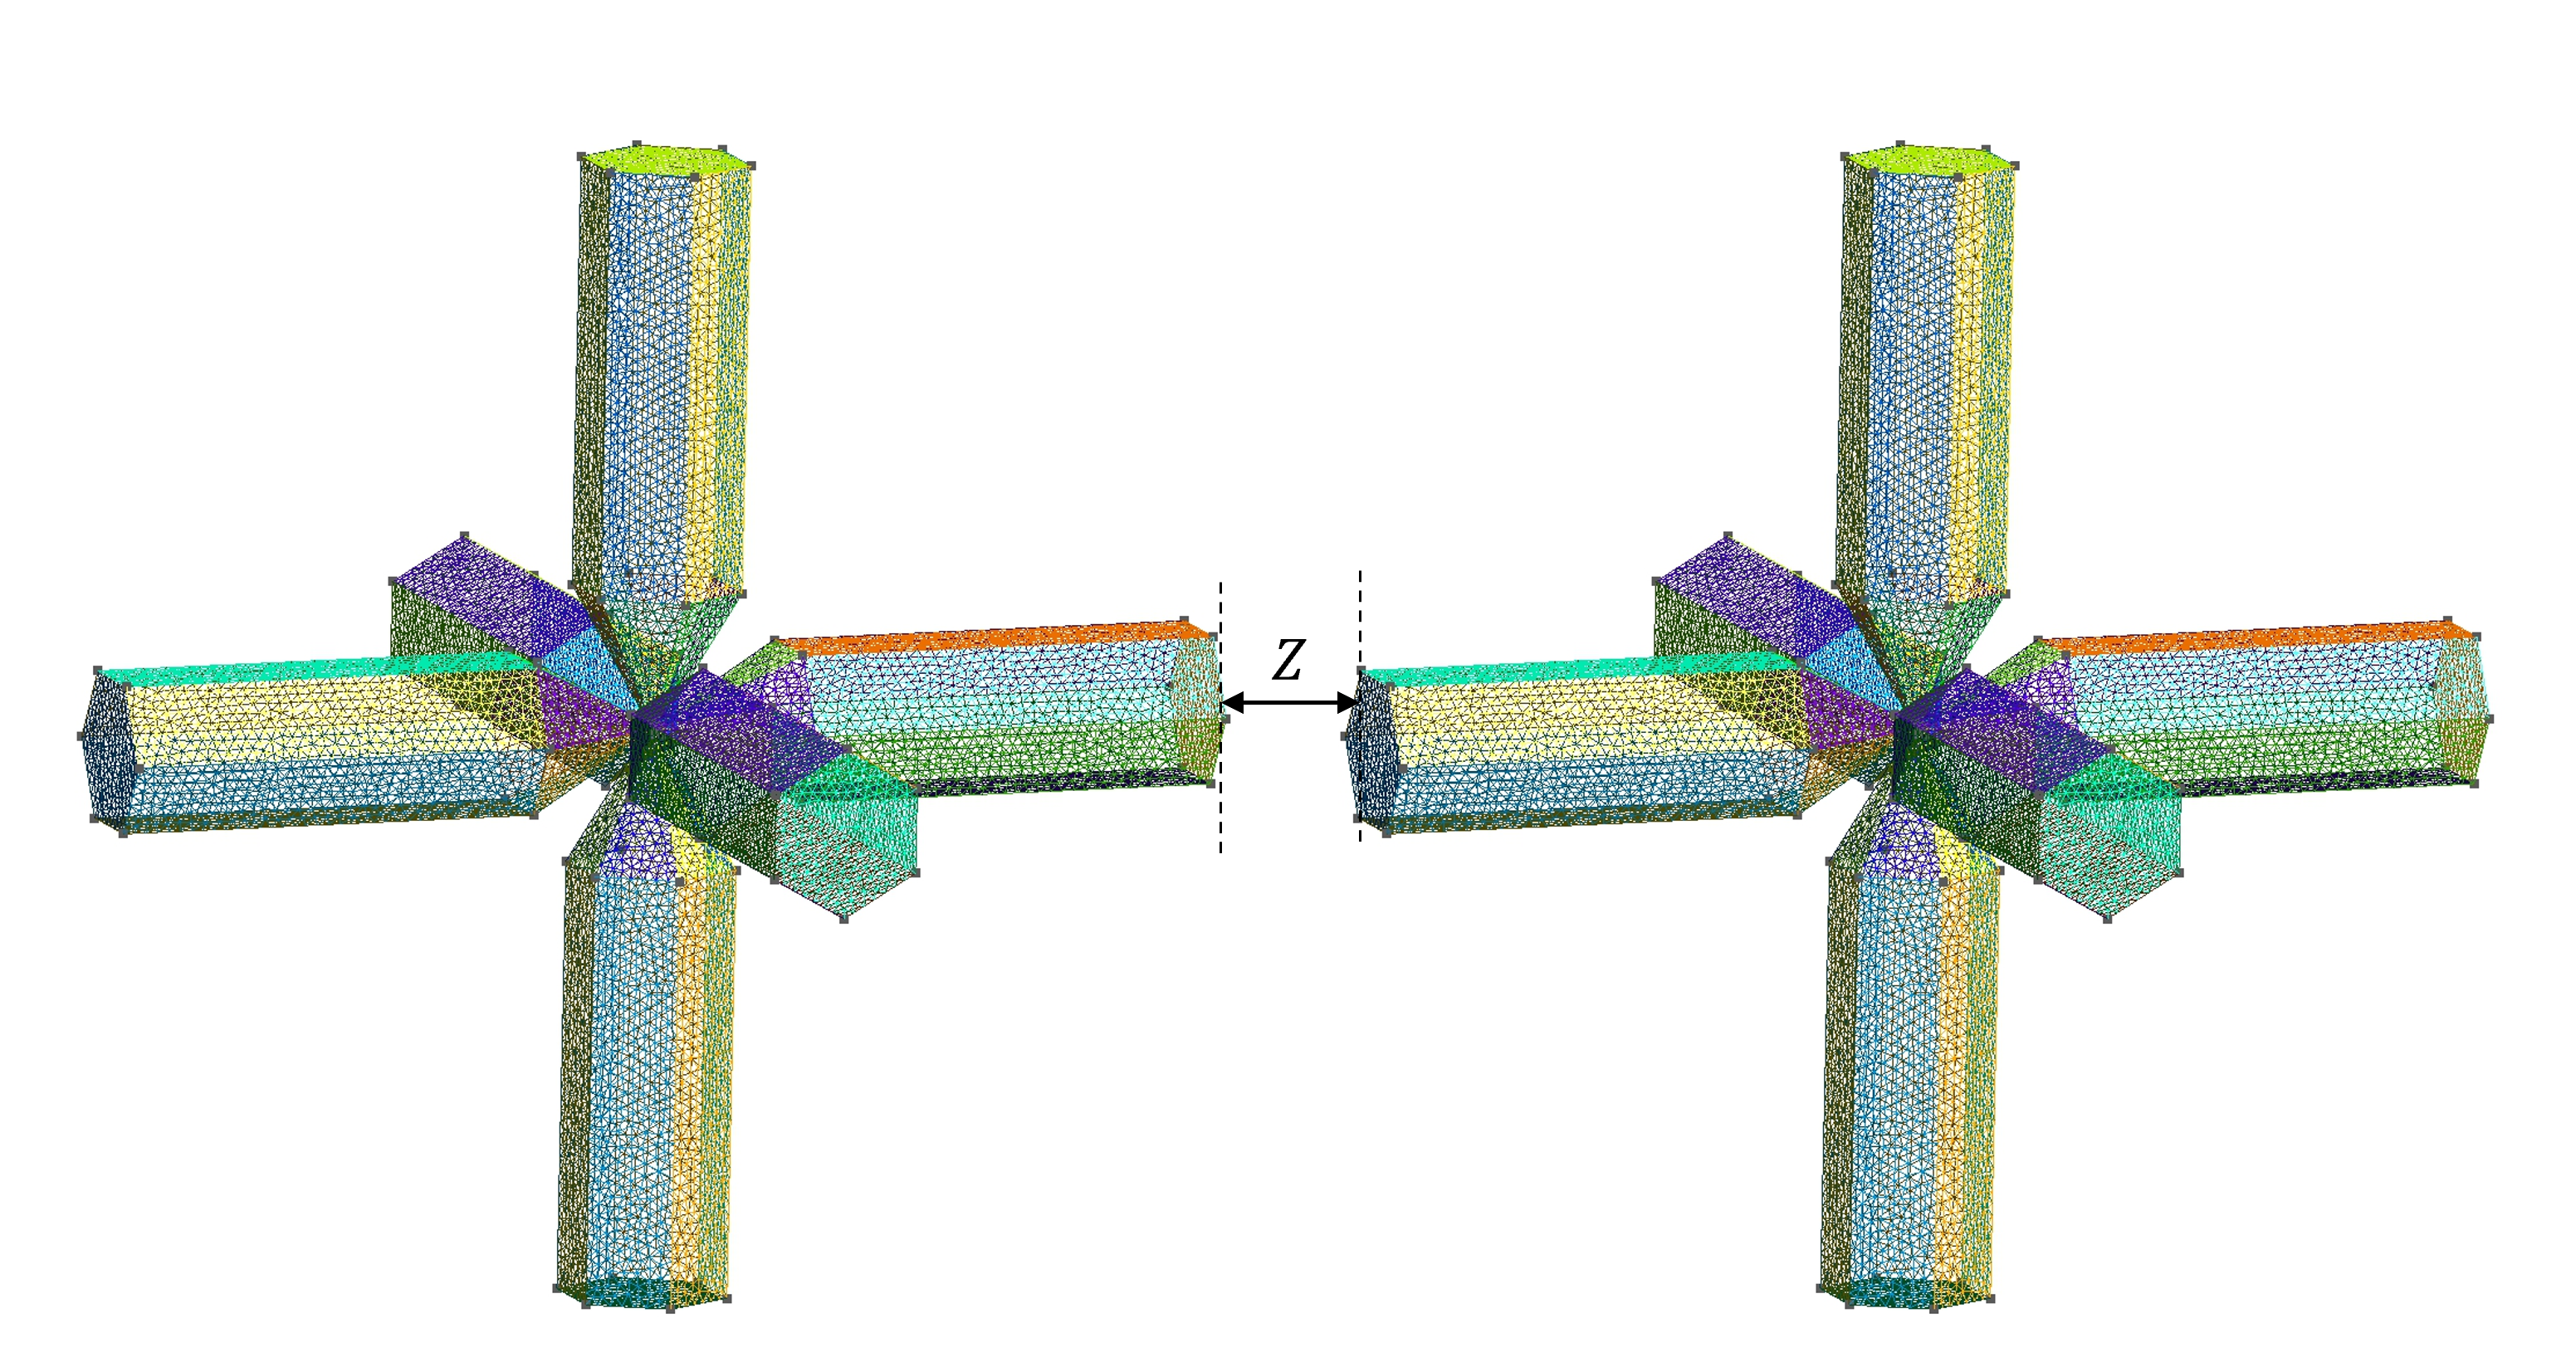
\includegraphics[scale = 0.4]{figures/6branches}
    %\caption{Six branches: $\text{dim}(\mathsf{V}_{\mathrm{i}k}) = 26262$ \newline N\textsuperscript{\underline{o}} of elements on both grids $ = 52556$}
    %\end{subfigure}
    \hspace*{1.5cm}
    \captionsetup[subfigure]{oneside,margin={1.2cm,0cm}}
    \subfloat[Six branches: $\text{dim}(\mathsf{V}_{\mathrm{i}k}) = 26262$ \newline N\textsuperscript{\underline{o}} of elements on both grids $ = 52556$]{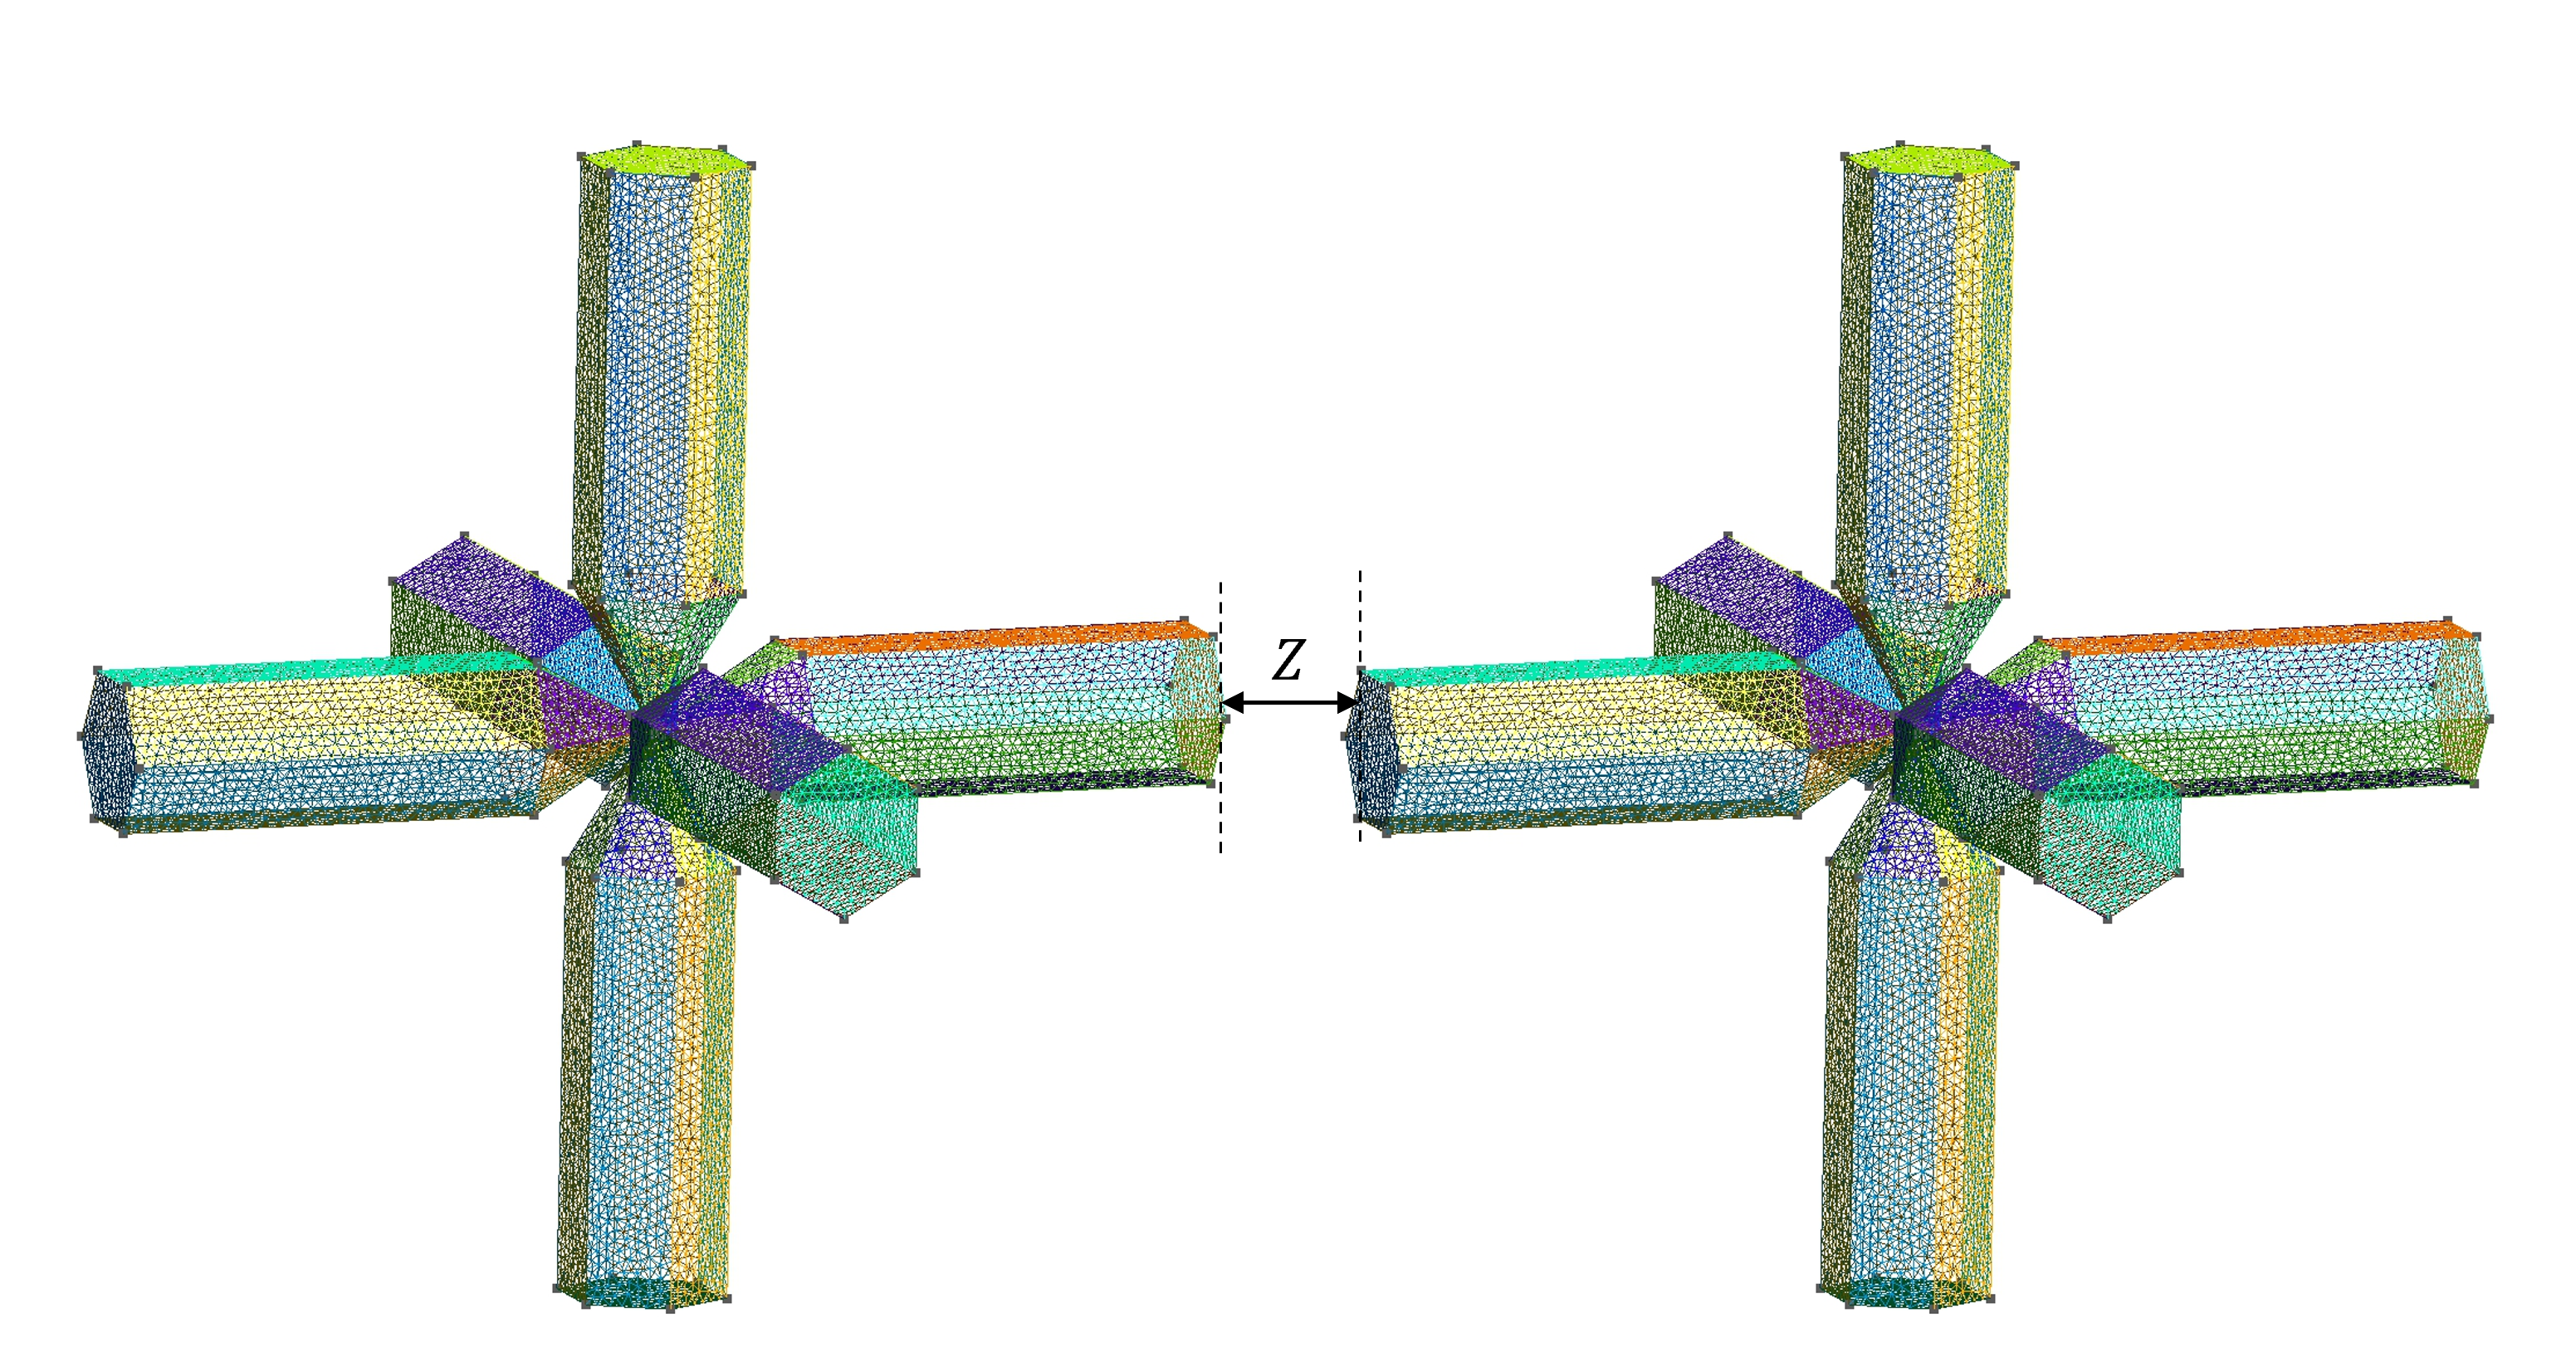
\includegraphics[scale=0.4]{figures/6branches}}
    \caption{Ice crystals with different number of branches}
    \label{Ice crystals with different number of branches}
    \end{figure}

    \begin{table}[H]
        \centering
        \begin{tabular}{ |P{2cm}||p{2cm}|p{2cm}|p{2cm}|p{2cm}|p{2cm}|  }
            \hline
            \multicolumn{6}{|c|}{Negative normalized Casimir energy in ice crystals' case} \\
            \hline
            Distance & 2-branches & 3-branches & 4-branches & 5-branches & 6-branches\\
            \hline
            0.5   & 0.04112    & 0.05989    & 0.07848   & 0.07873    & 0.01128\\
            0.75  & 0.01499    & 0.02184    & 0.02855   & 0.02873    & 0.005017\\
            1.0   & 0.007403   & 0.01080    & 0.01412   & 0.01428    & 0.002965\\
            1.25  & 0.004242   & 0.006198   & 0.008113  & 0.008242   & 0.001985\\
            1.5   & 0.002672   & 0.003905   & 0.005117  & 0.005223   & 0.001427\\
            1.75  & 0.001797   & 0.002624   & 0.003442  & 0.003530   & 0.001074\\
            2.0   & 0.001268   & 0.001849   & 0.002428  & 0.002501   & 0.0008357\\
            2.25  & 0.0009288  & 0.001353   & 0.001776  & 0.001839   & 0.0006664\\
            2.5   & 0.0007007  & 0.001019   & 0.001338  & 0.001391   & 0.0005410\\
            2.75  & 0.0005413  & 0.0007863  & 0.001033  & 0.001078   & 0.0004469\\
            3.0   & 0.0004270  & 0.0006188  & 0.0008134 & 0.0008526  & 0.0003741\\
            \hline
           \end{tabular}
           \caption{\label{Negative normalized Casimir energy in ice crystals' case table} Negative normalized Casimir energy in 2- to 6-branched ice crystals' case}
        \end{table}

        \begin{figure}[H]
            \centering
            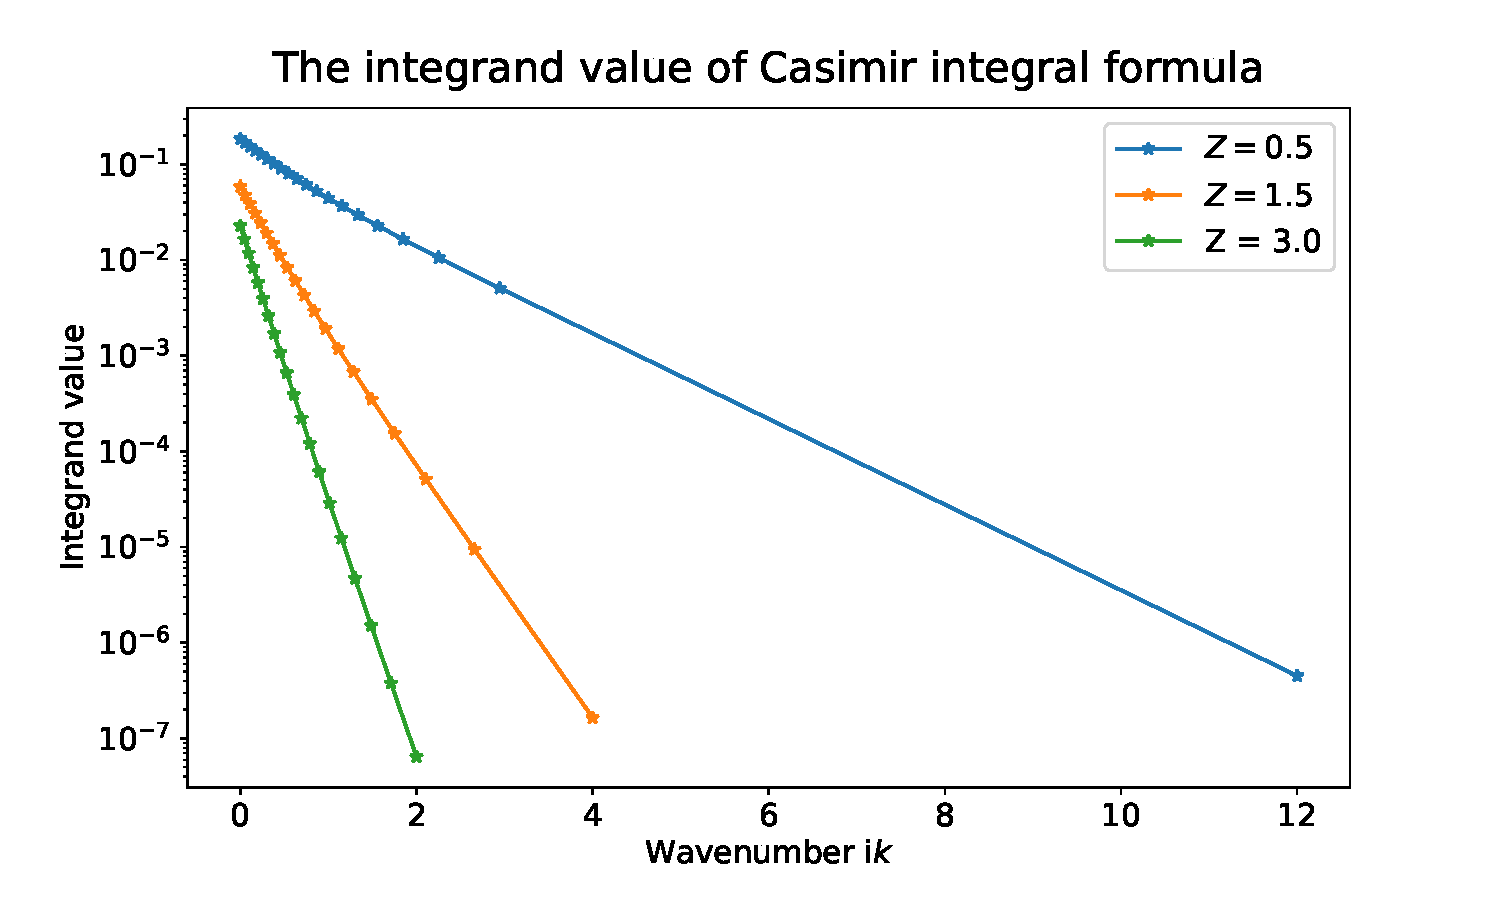
\includegraphics[scale = 1]{figures/5branches_integrand_Value.png}
            \caption{The integrand of the Casimir energy between two five-branches ice crystals with distance $Z = 0.5$, 1.5 and 3.0.}      
              \end{figure}
        
        \begin{figure}[H]
                \centering
                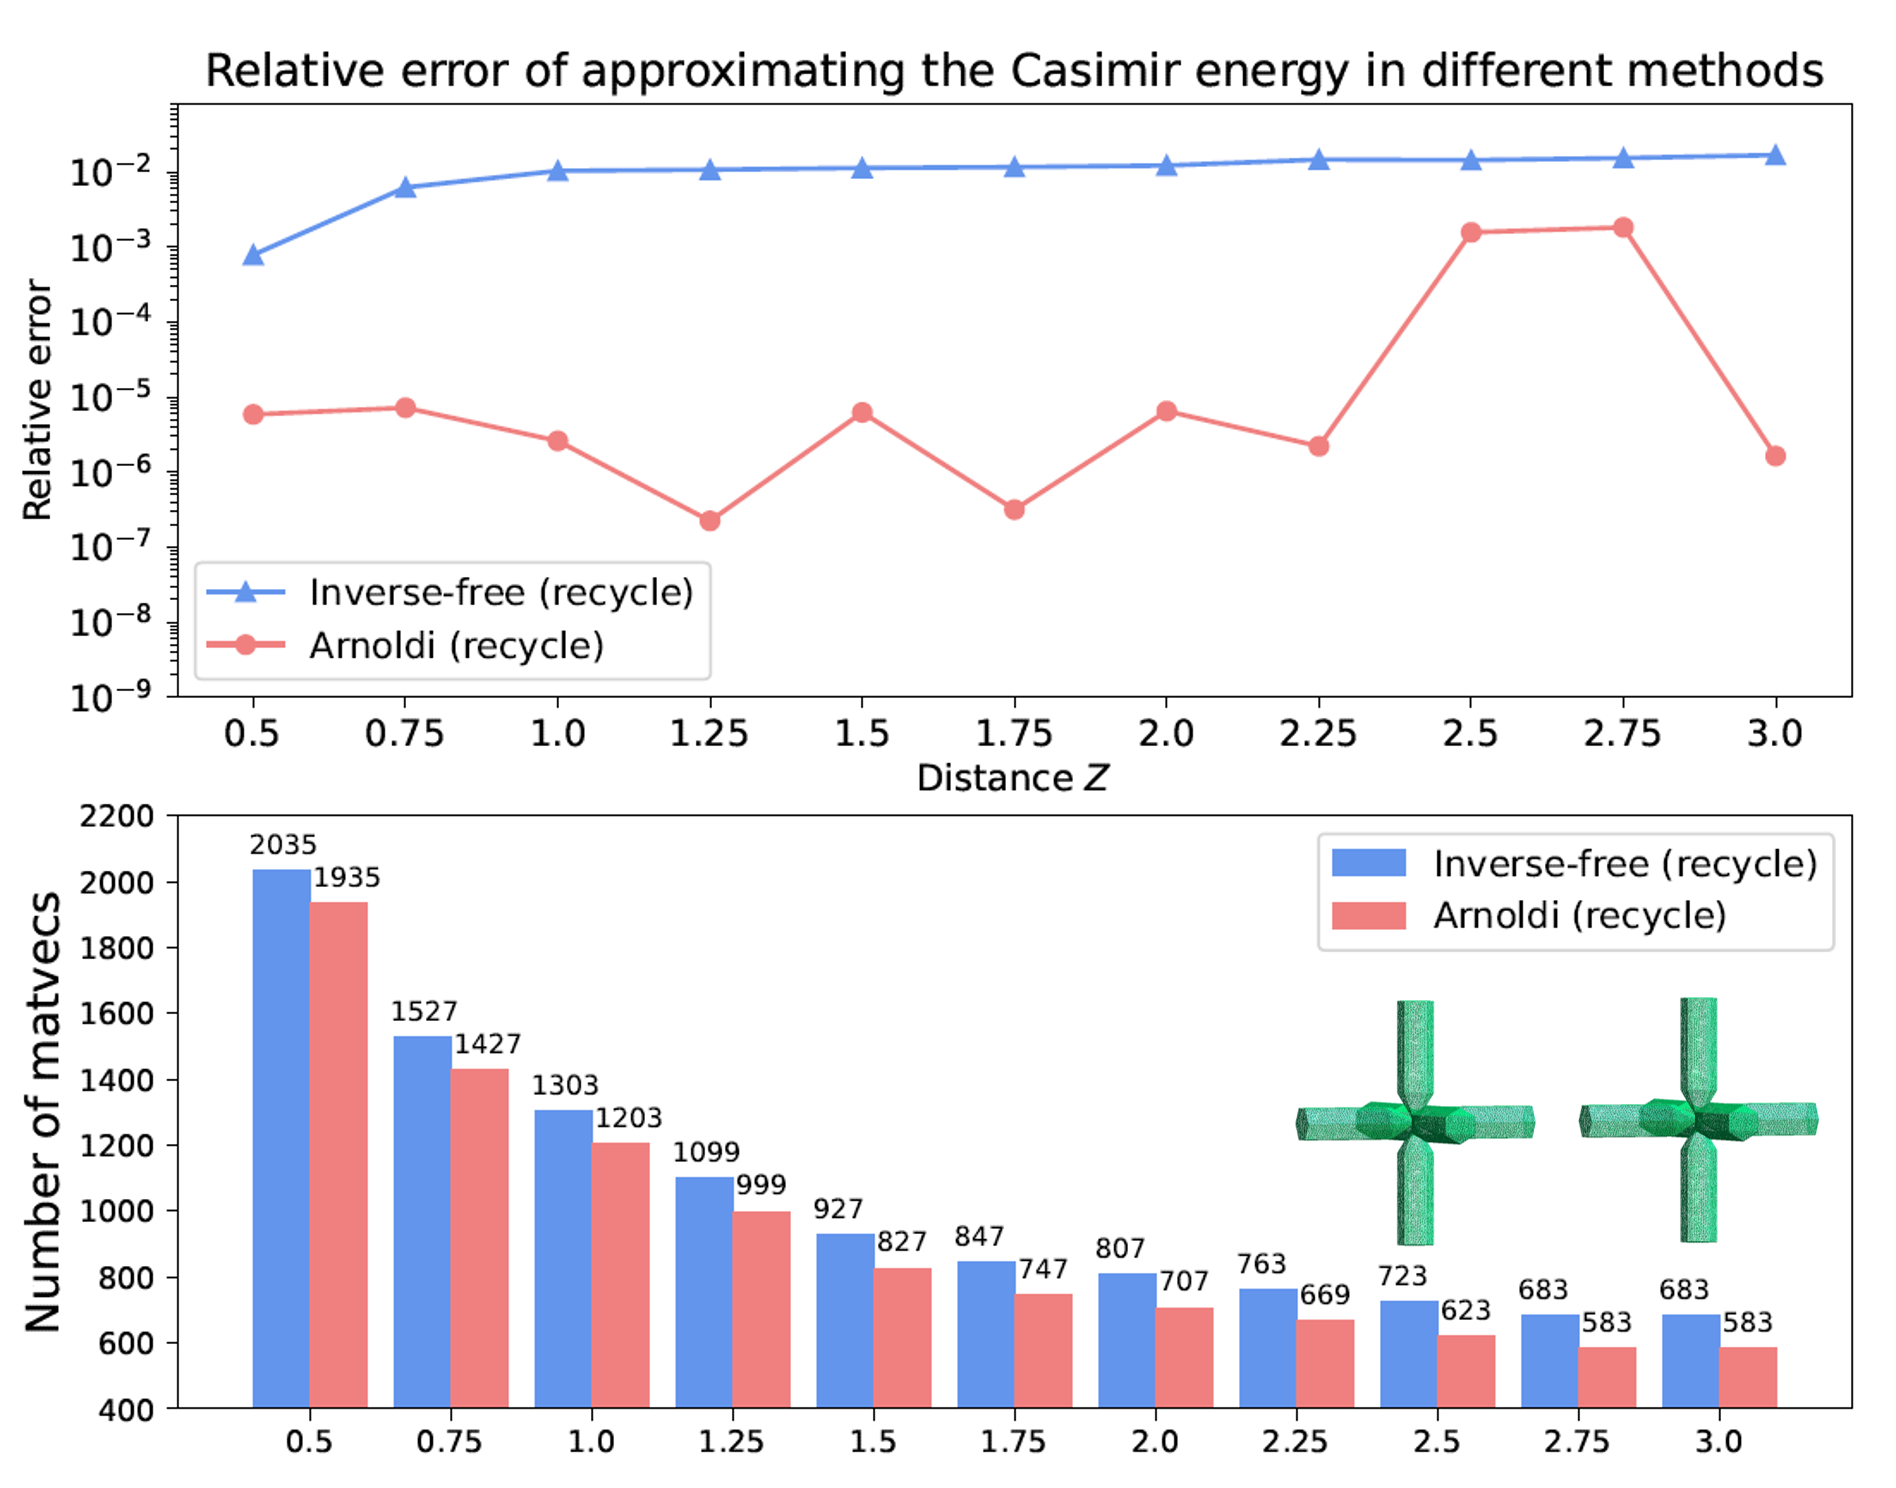
\includegraphics[width = \textwidth]{figures/6branches_rel_err.png}
                \caption{Six-branches ice crystals' case: relative distance between the reference value (computed by Richardson extrapolation) with the estimates evaluated from the standard Arnoldi 
                method with subspace recycled (solid red circles) and inverse-free Krylov subspace method with subspace recycled (solid blue triangles). The dimension of the Krylov subspace is $m = 100$.
                The recycled eigenvector has the corresponding eigenvalue whose logarithm is larger than $10^{-5}$.}       
             \end{figure}
% For large problems, we can apply the fast multipole method method (FMM)\cite{ying2004kernel} when discretizing the operators. Compared with the dense assembly, it reduces 
% the storage memory and also speed up the matrix assembly. Although it takes longer when multiplying the matrix assembled by FMM with the vectors, 
% the decreasing number of the matrix-vector products (see Figure \ref{running_time_fmm} (Right)) leads to a shorter running time for computing the $\log\det(\mathsf{V}(\mathrm{i}k)\tilde{\mathsf{V}}(\mathrm{i}k)^{-1})$
% (see Figure \ref{running_time_fmm} (Left)). 
% \begin{figure}[H]
%     \centering
%     \hspace*{-1.5cm}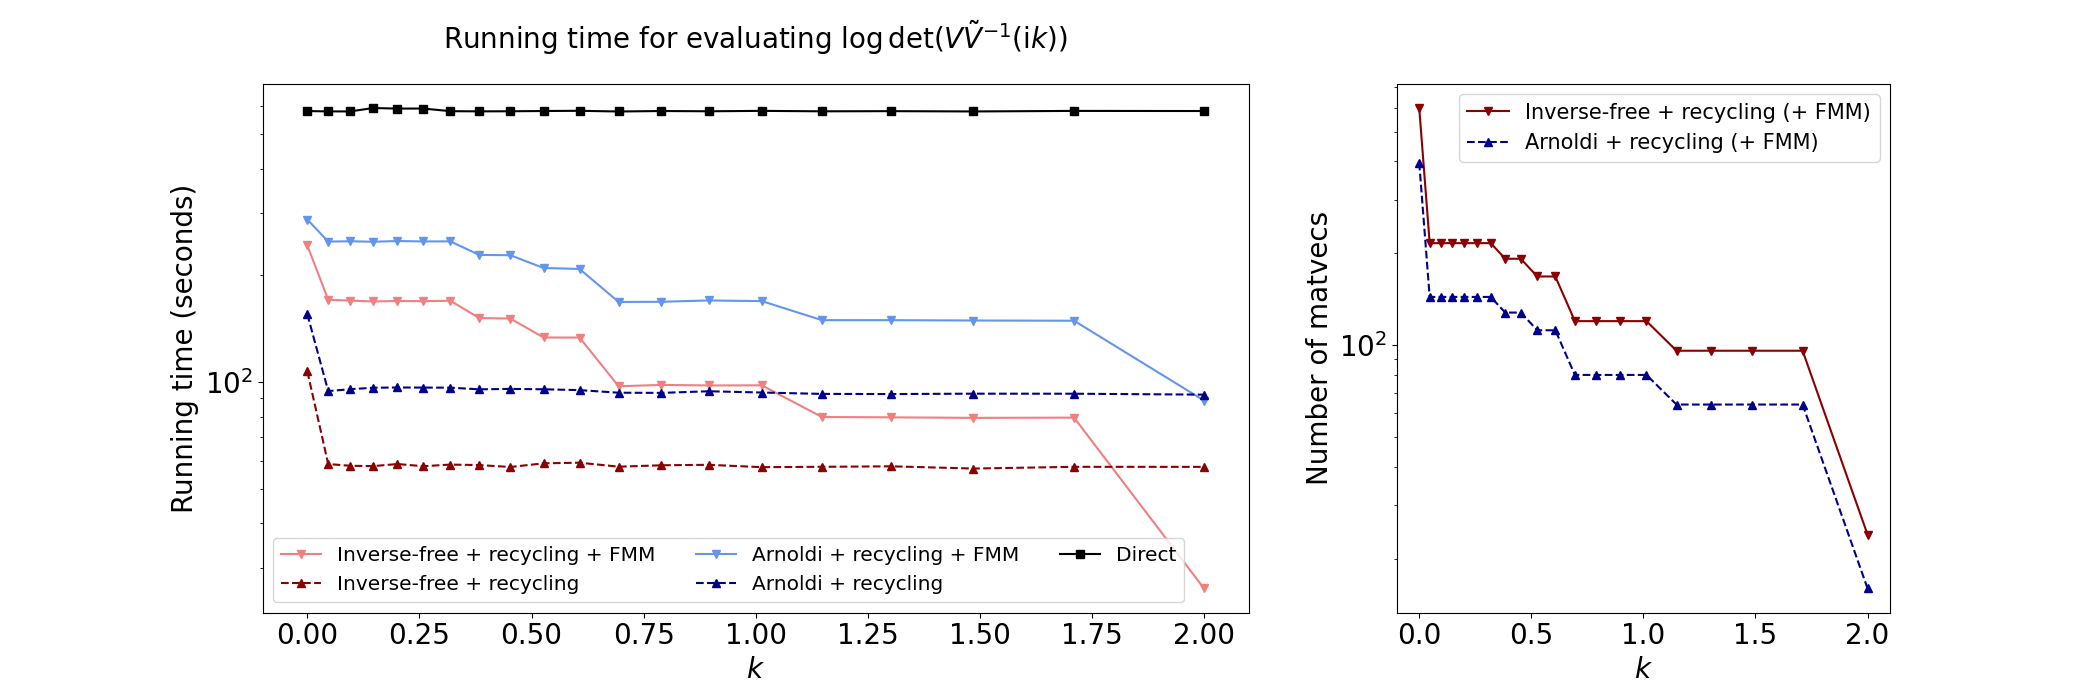
\includegraphics[width = 1.2\textwidth]{figures/running_time_fmm.png}
%     \caption{Six-branches ice crystals' case: (Left) running time for evaluating the $\log\det(\mathsf{V}(\mathrm{i}k)\tilde{\mathsf{V}}(\mathrm{i}k)^{-1})$ by
%     the direct dense computation and the recycling approaches with/without implementing FMM. The expansion order for FMM is 7. 
%     (Right) The number of the matrix-vector products in the recycling approaches with/without implementing FMM for each wavenumber case.}
%     \label{running_time_fmm}
% \end{figure}        
        %==================================================================================================
It is not hard to imagine that the Casimir energy would be different when rotating the scatterers and keeping the distance between them unchanged. Therefore, 
in the last example, we would see how the Casimir energy between two identical ellipsoids changes as one of the ellipsoids rotates.

In Figure \ref{Without rotation}, the above ellipsoid is centering at $(0,0,0)$ and the below one is centering at $(0, 0, -(0.5+0.5+Z))$, where $Z$ is the 
distance between these two ellipsoids. Without rotation, the Casimir energy between them with different distance $Z$ is plotted in Figure 
\ref{Casimir energy between two ellipsoids with different distances}.

To explore how the rotation affects the change of the Casimir energy, one can always keep one ellipsoid fixed and rotate the other one. The Figure 
\ref{Rotation around z-axis} and \ref{Rotation around x-axis} describe the case when one of the ellipsoids rotates around $z-$ and $x-$axis, respectively.
From the Figure \ref{Casimir energy when one of the ellipsoids rotates}, the Casimir energy changes periodically since we rotate one ellipsoid around 
$z-$ or $x-$axis by 360 degrees. 


\begin{figure}[H]
    \begin{subfigure}{\linewidth}
        \centering
        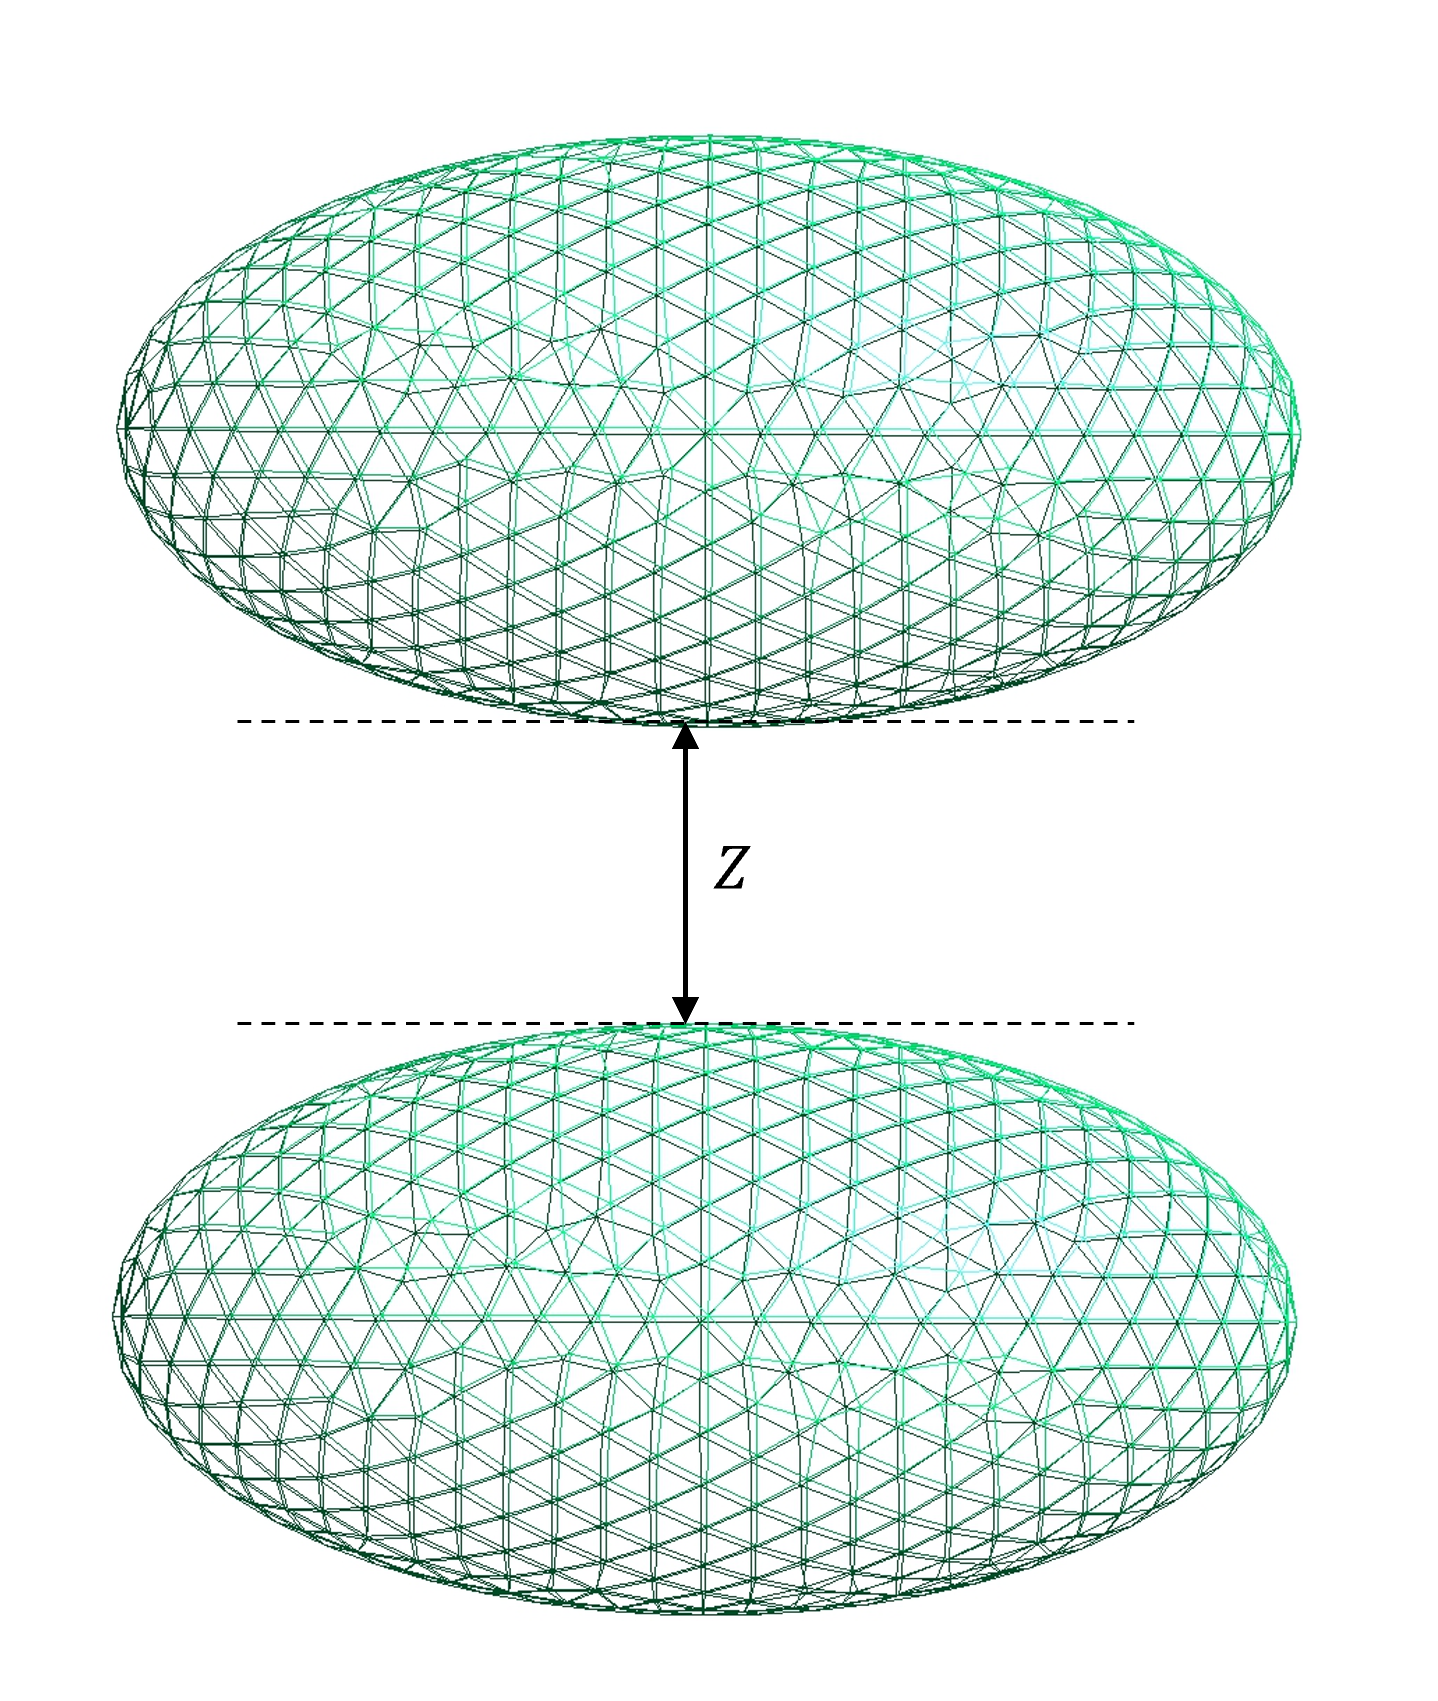
\includegraphics[scale = 0.3]{figures/two_ellipsoids}
        \caption{Without rotation}
        \label{Without rotation}
        \end{subfigure}\\[1ex]
    \begin{subfigure}[t]{.5\linewidth}
    \centering
    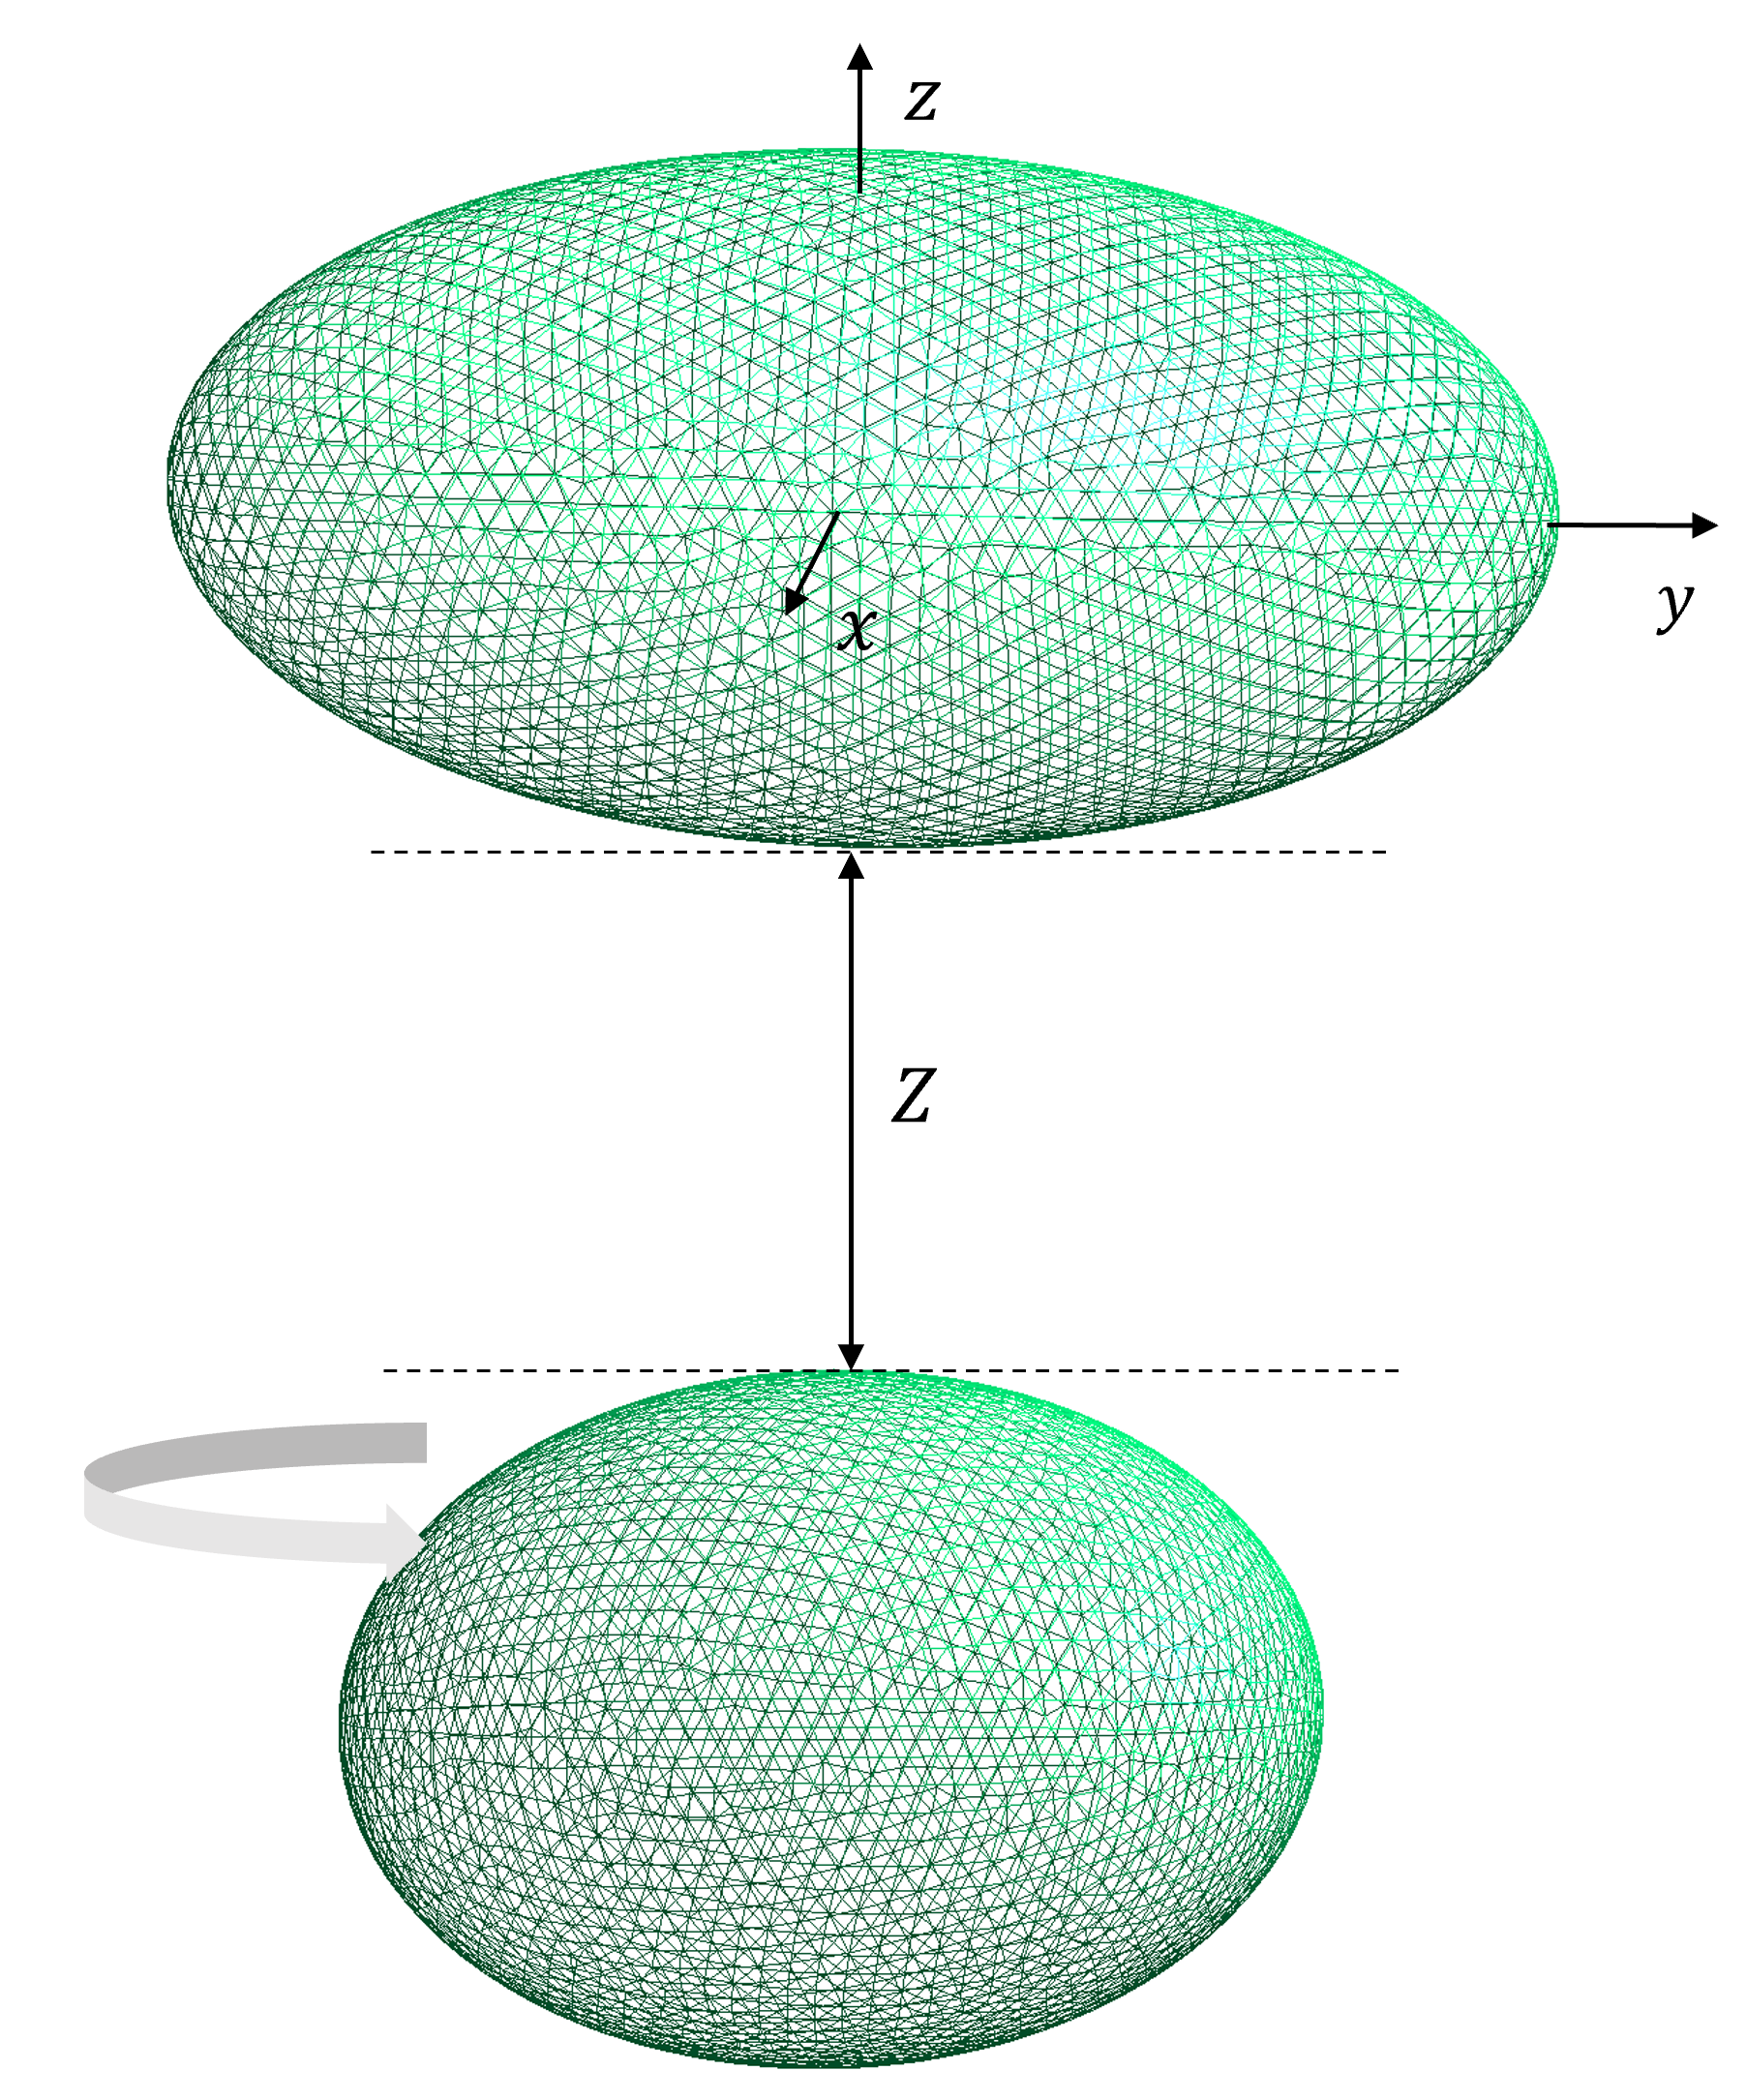
\includegraphics[scale = 0.3]{figures/Ellipsoid_z_axis}
    \caption{Rotation around z-axis}
    \label{Rotation around z-axis}
    \end{subfigure}%
    \begin{subfigure}[t]{.5\linewidth}
    \centering
    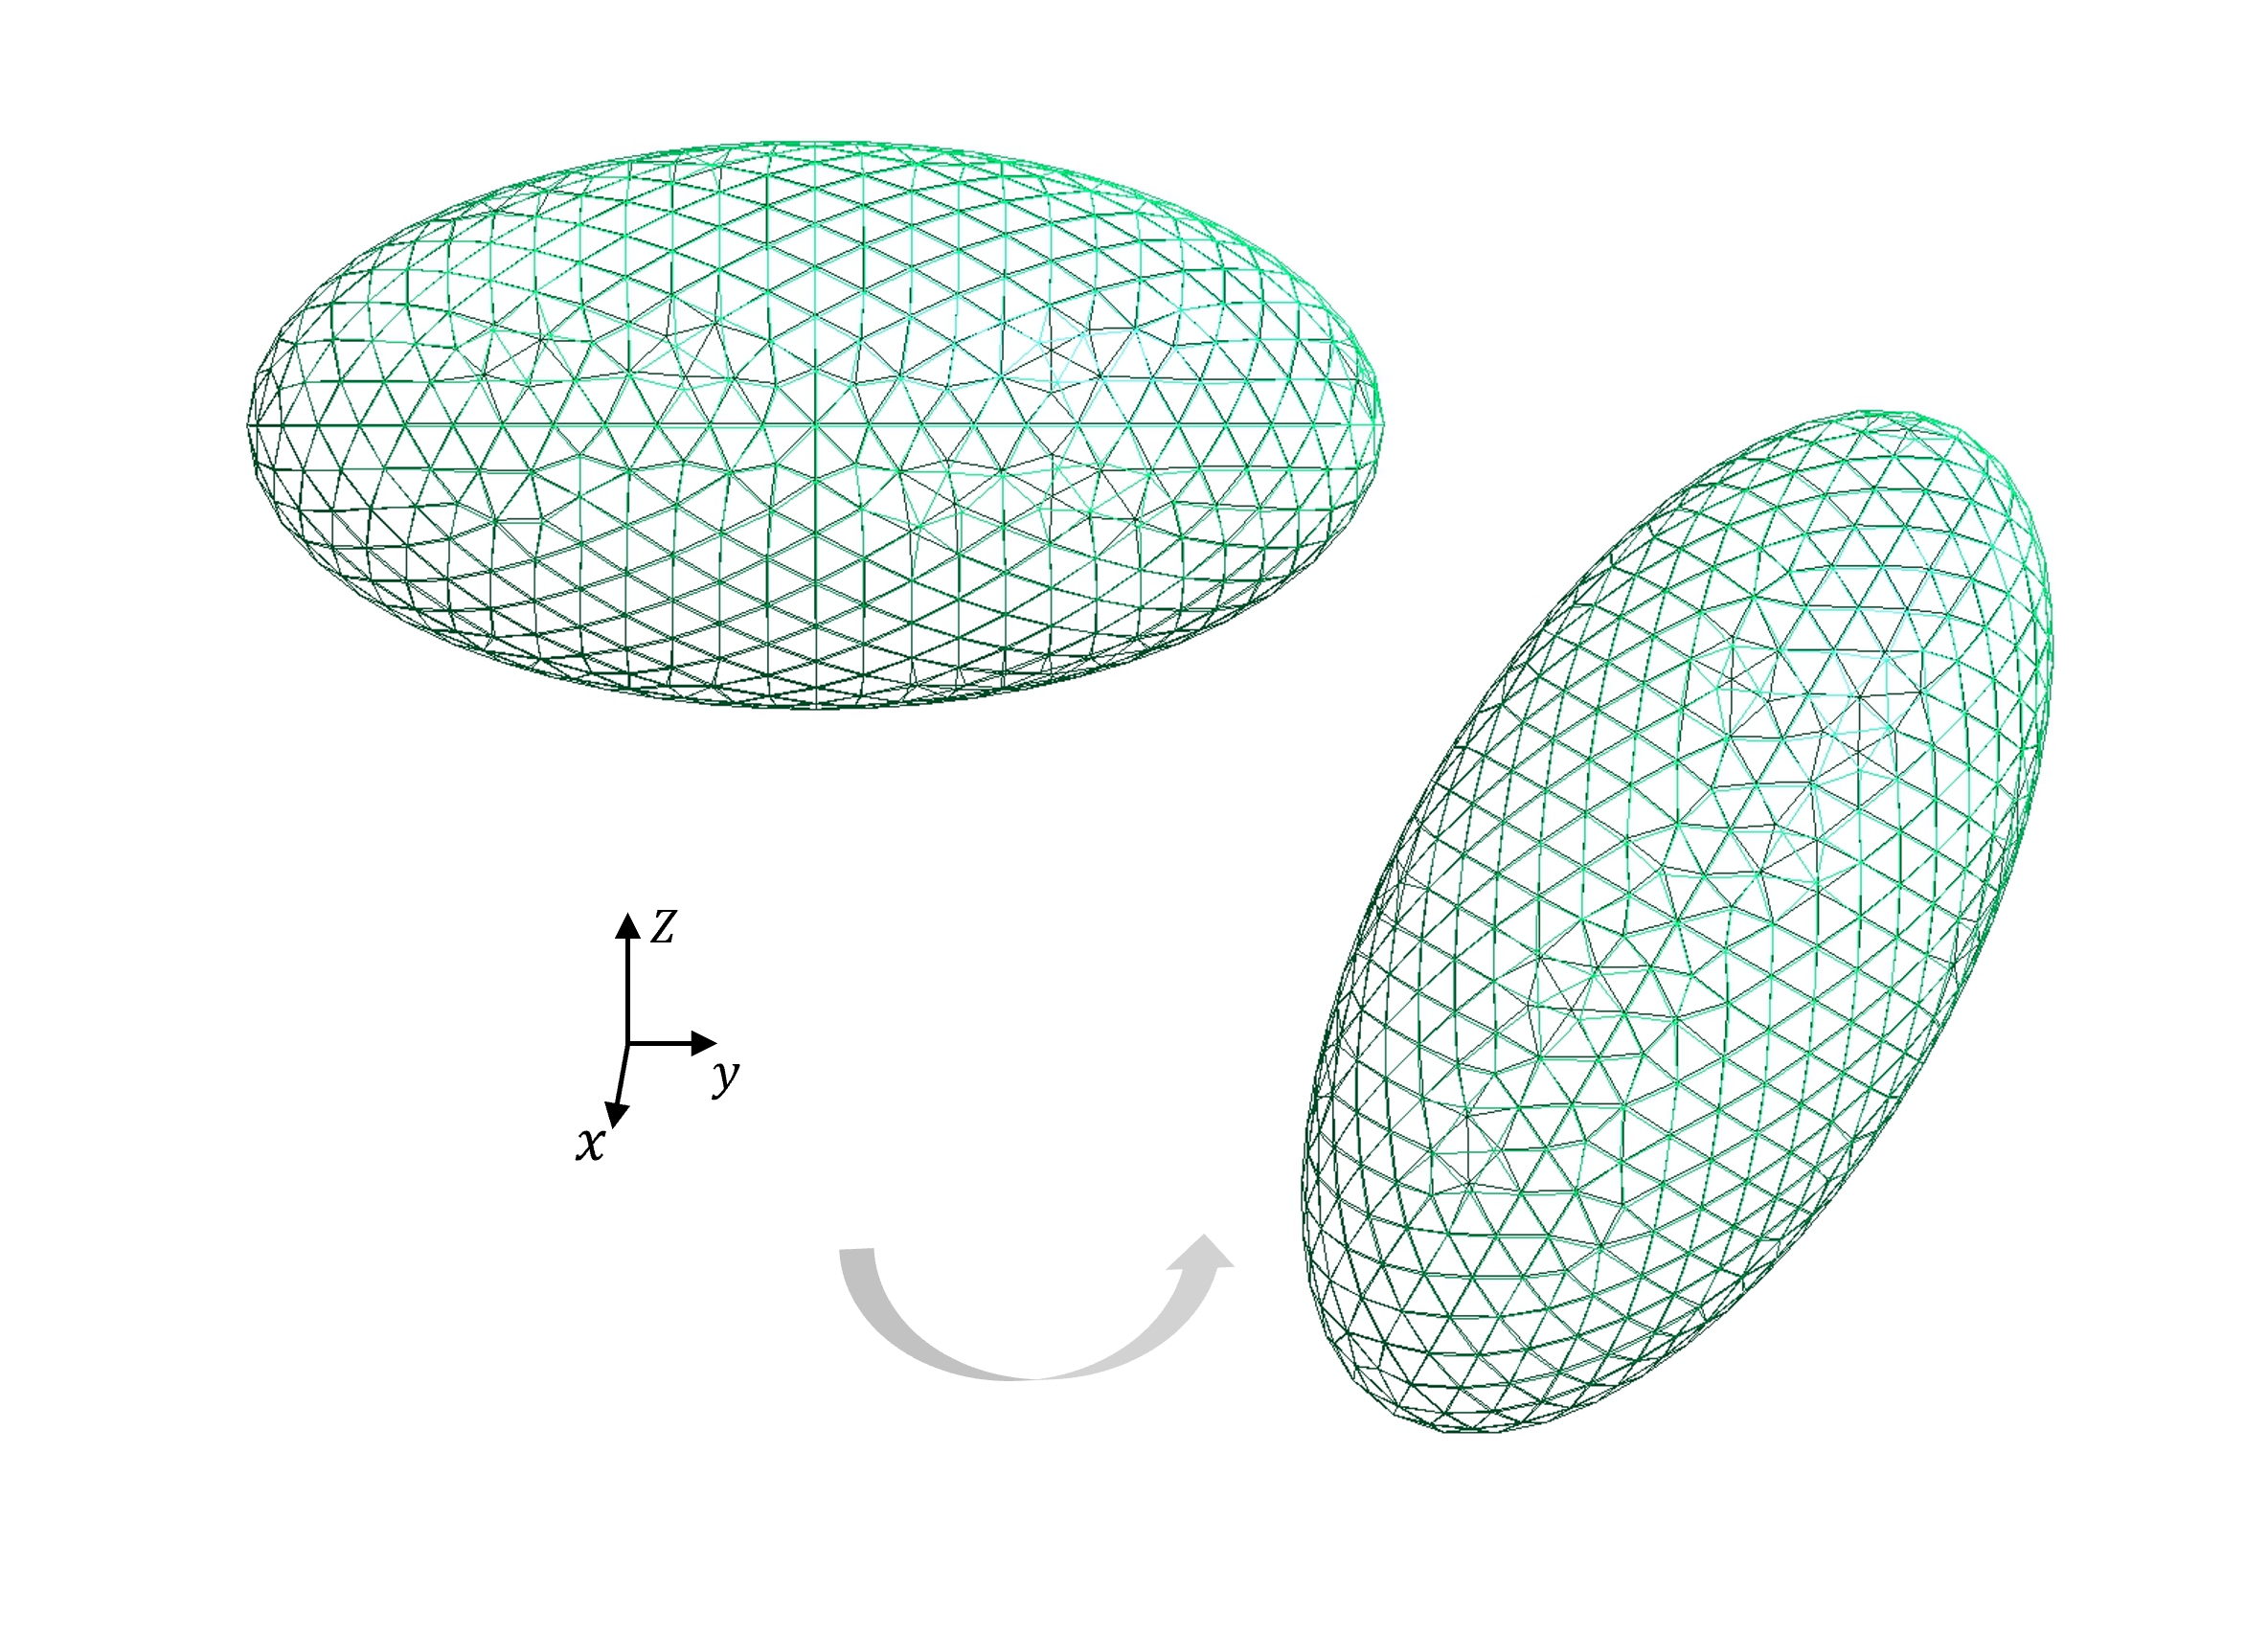
\includegraphics[scale = 0.07]{figures/Ellipsoid_x_axis}
    \caption{Rotation around x-axis}
    \label{Rotation around x-axis}
    \end{subfigure}
    \caption{Two ellipsoids with or without rotation: when $h_\text{fine}$ = 0.05, $\text{dim}(\mathsf{V}_{\mathrm{i}k}) = 5517$; 
    $h_\text{coarse}$ = 0.1, $\text{dim}(\mathsf{V}_{\mathrm{i}k}) = 1498$. The principal semi-axes of two ellipsoids are $r_{1} = 0.5$ and $r_{2} = 1.0$.}
    \label{Two ellipsoids}
    \end{figure}

    \begin{figure}[H]
        \begin{subfigure}{\linewidth}
            \centering
            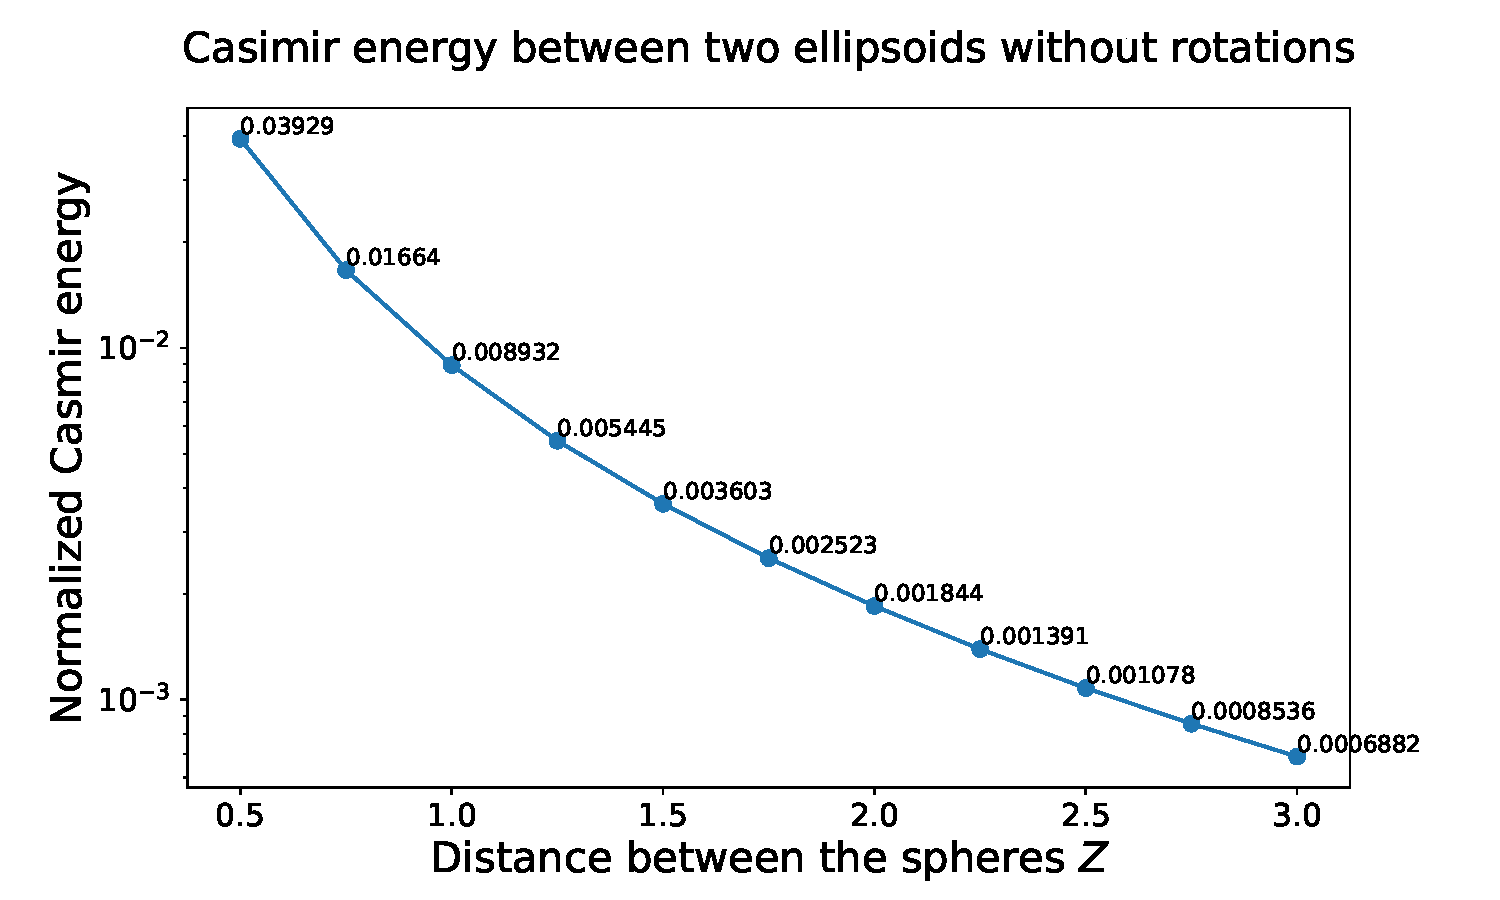
\includegraphics[scale = 0.5]{figures/CasE_ellipsoids.pdf}
            \caption{Casimir energy between two ellipsoids with different distances}
            \label{Casimir energy between two ellipsoids with different distances}
            \end{subfigure}\\[1ex]
    
        \begin{subfigure}{\linewidth}
        \centering
        \hspace*{-1cm}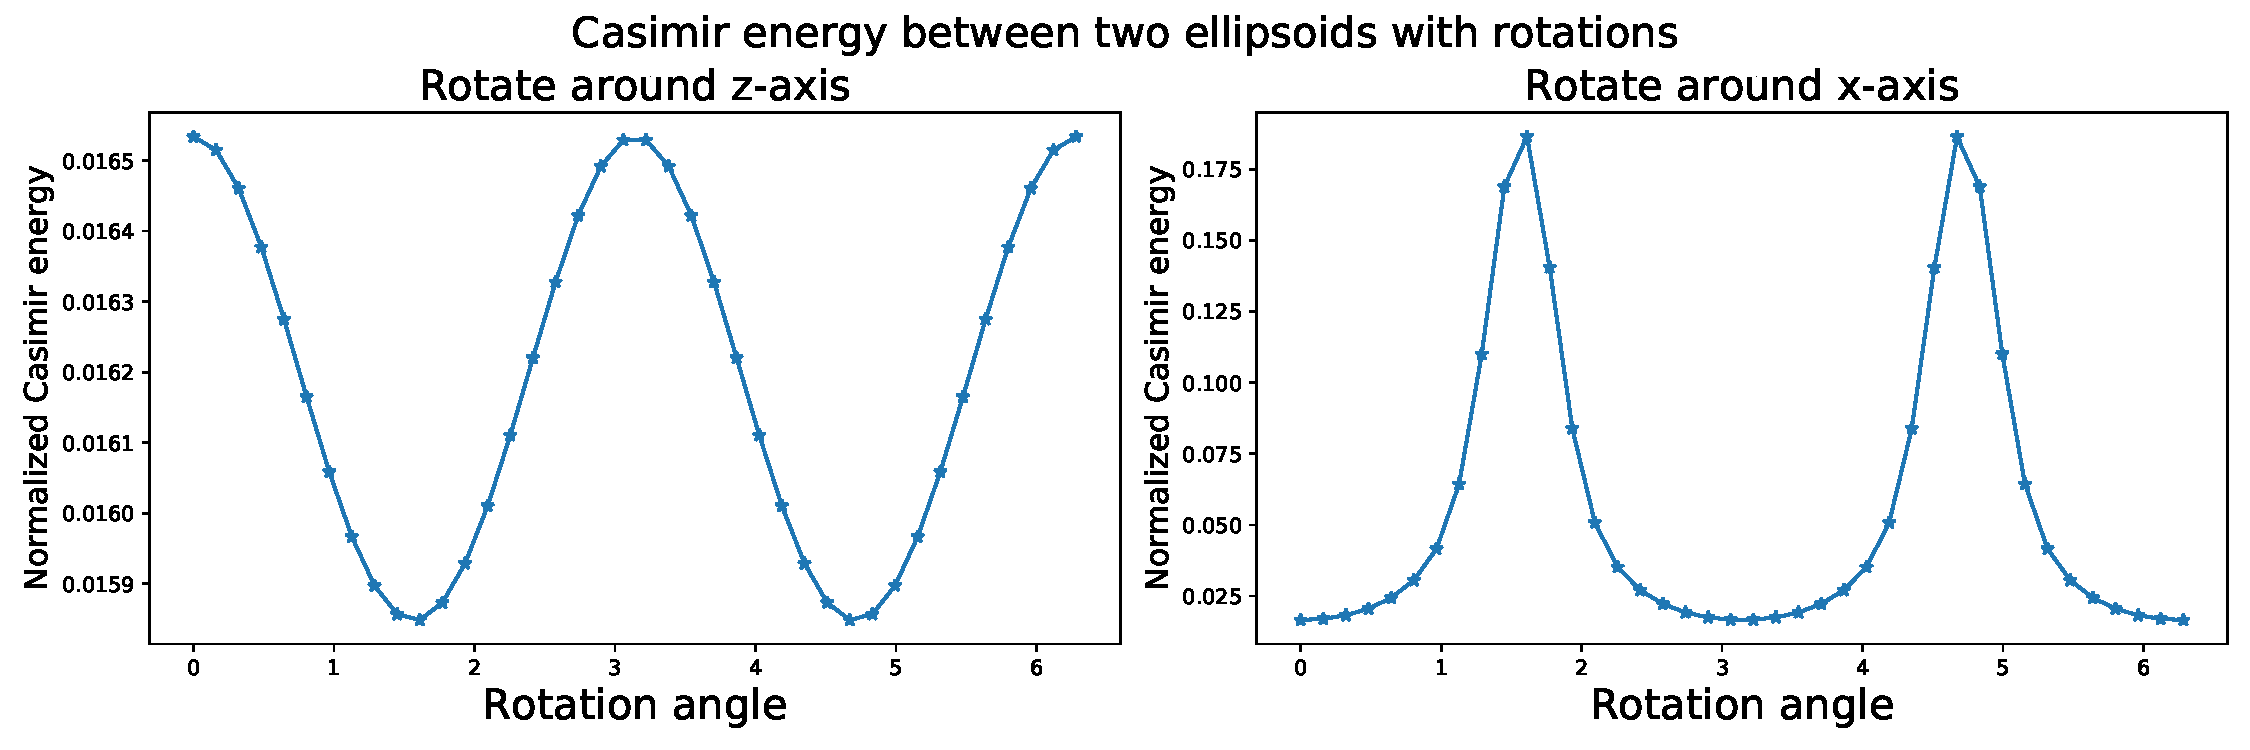
\includegraphics[scale = 0.45]{figures/CasE_ellipsoids_with_rotation.pdf}
        \caption{Casimir energy when one of the ellipsoids rotates}
        \label{Casimir energy when one of the ellipsoids rotates}
        \end{subfigure}
        \caption{The dependence of the Casimir energy and rotation angle of one of the ellipsoids.} 
        \end{figure}

Now, consider 4 ellipsoids located on the vertices of a regular tetrahedron with edge length $l = 2$ (Figure \ref{Four ellipsoids with or without rotations}) and 
the principal semi-axes of all these ellipsoids are $r_{1} = 0.6$ and $r_{2} = 0.3$. Figure \ref{Rotation inwards 4} and Figure \ref{Rotation outwards 4}
show the rotation of the ellipsoids inwards and outwards 360 degrees towards the centroid of this tetrahedron, separately. Afterwards, in order to use the Richardson extrapolation
method to estimate the Casimir energy, we evaluate the integral \eqref{KSSF and CasE} with the grid size set as $h_{\text{fine}} = 0.05$ and 
$h_{\text{coarse}} = 0.03$. Note that the number of the scatterers has increased to four, the matrices $\mathsf{V}_{\mathrm{i}k}$ and 
$\tilde{\mathsf{V}}_{\mathrm{i}k}$ have become to 4 by 4 block and diagonal block matrix, 
respectively. From the Figure \ref{Four ellipsoids}, it shows that the Casimir energy between these four ellipsoids changes periodically with the rotation.

\begin{figure}[H]
    \begin{subfigure}{\linewidth}
        \centering
        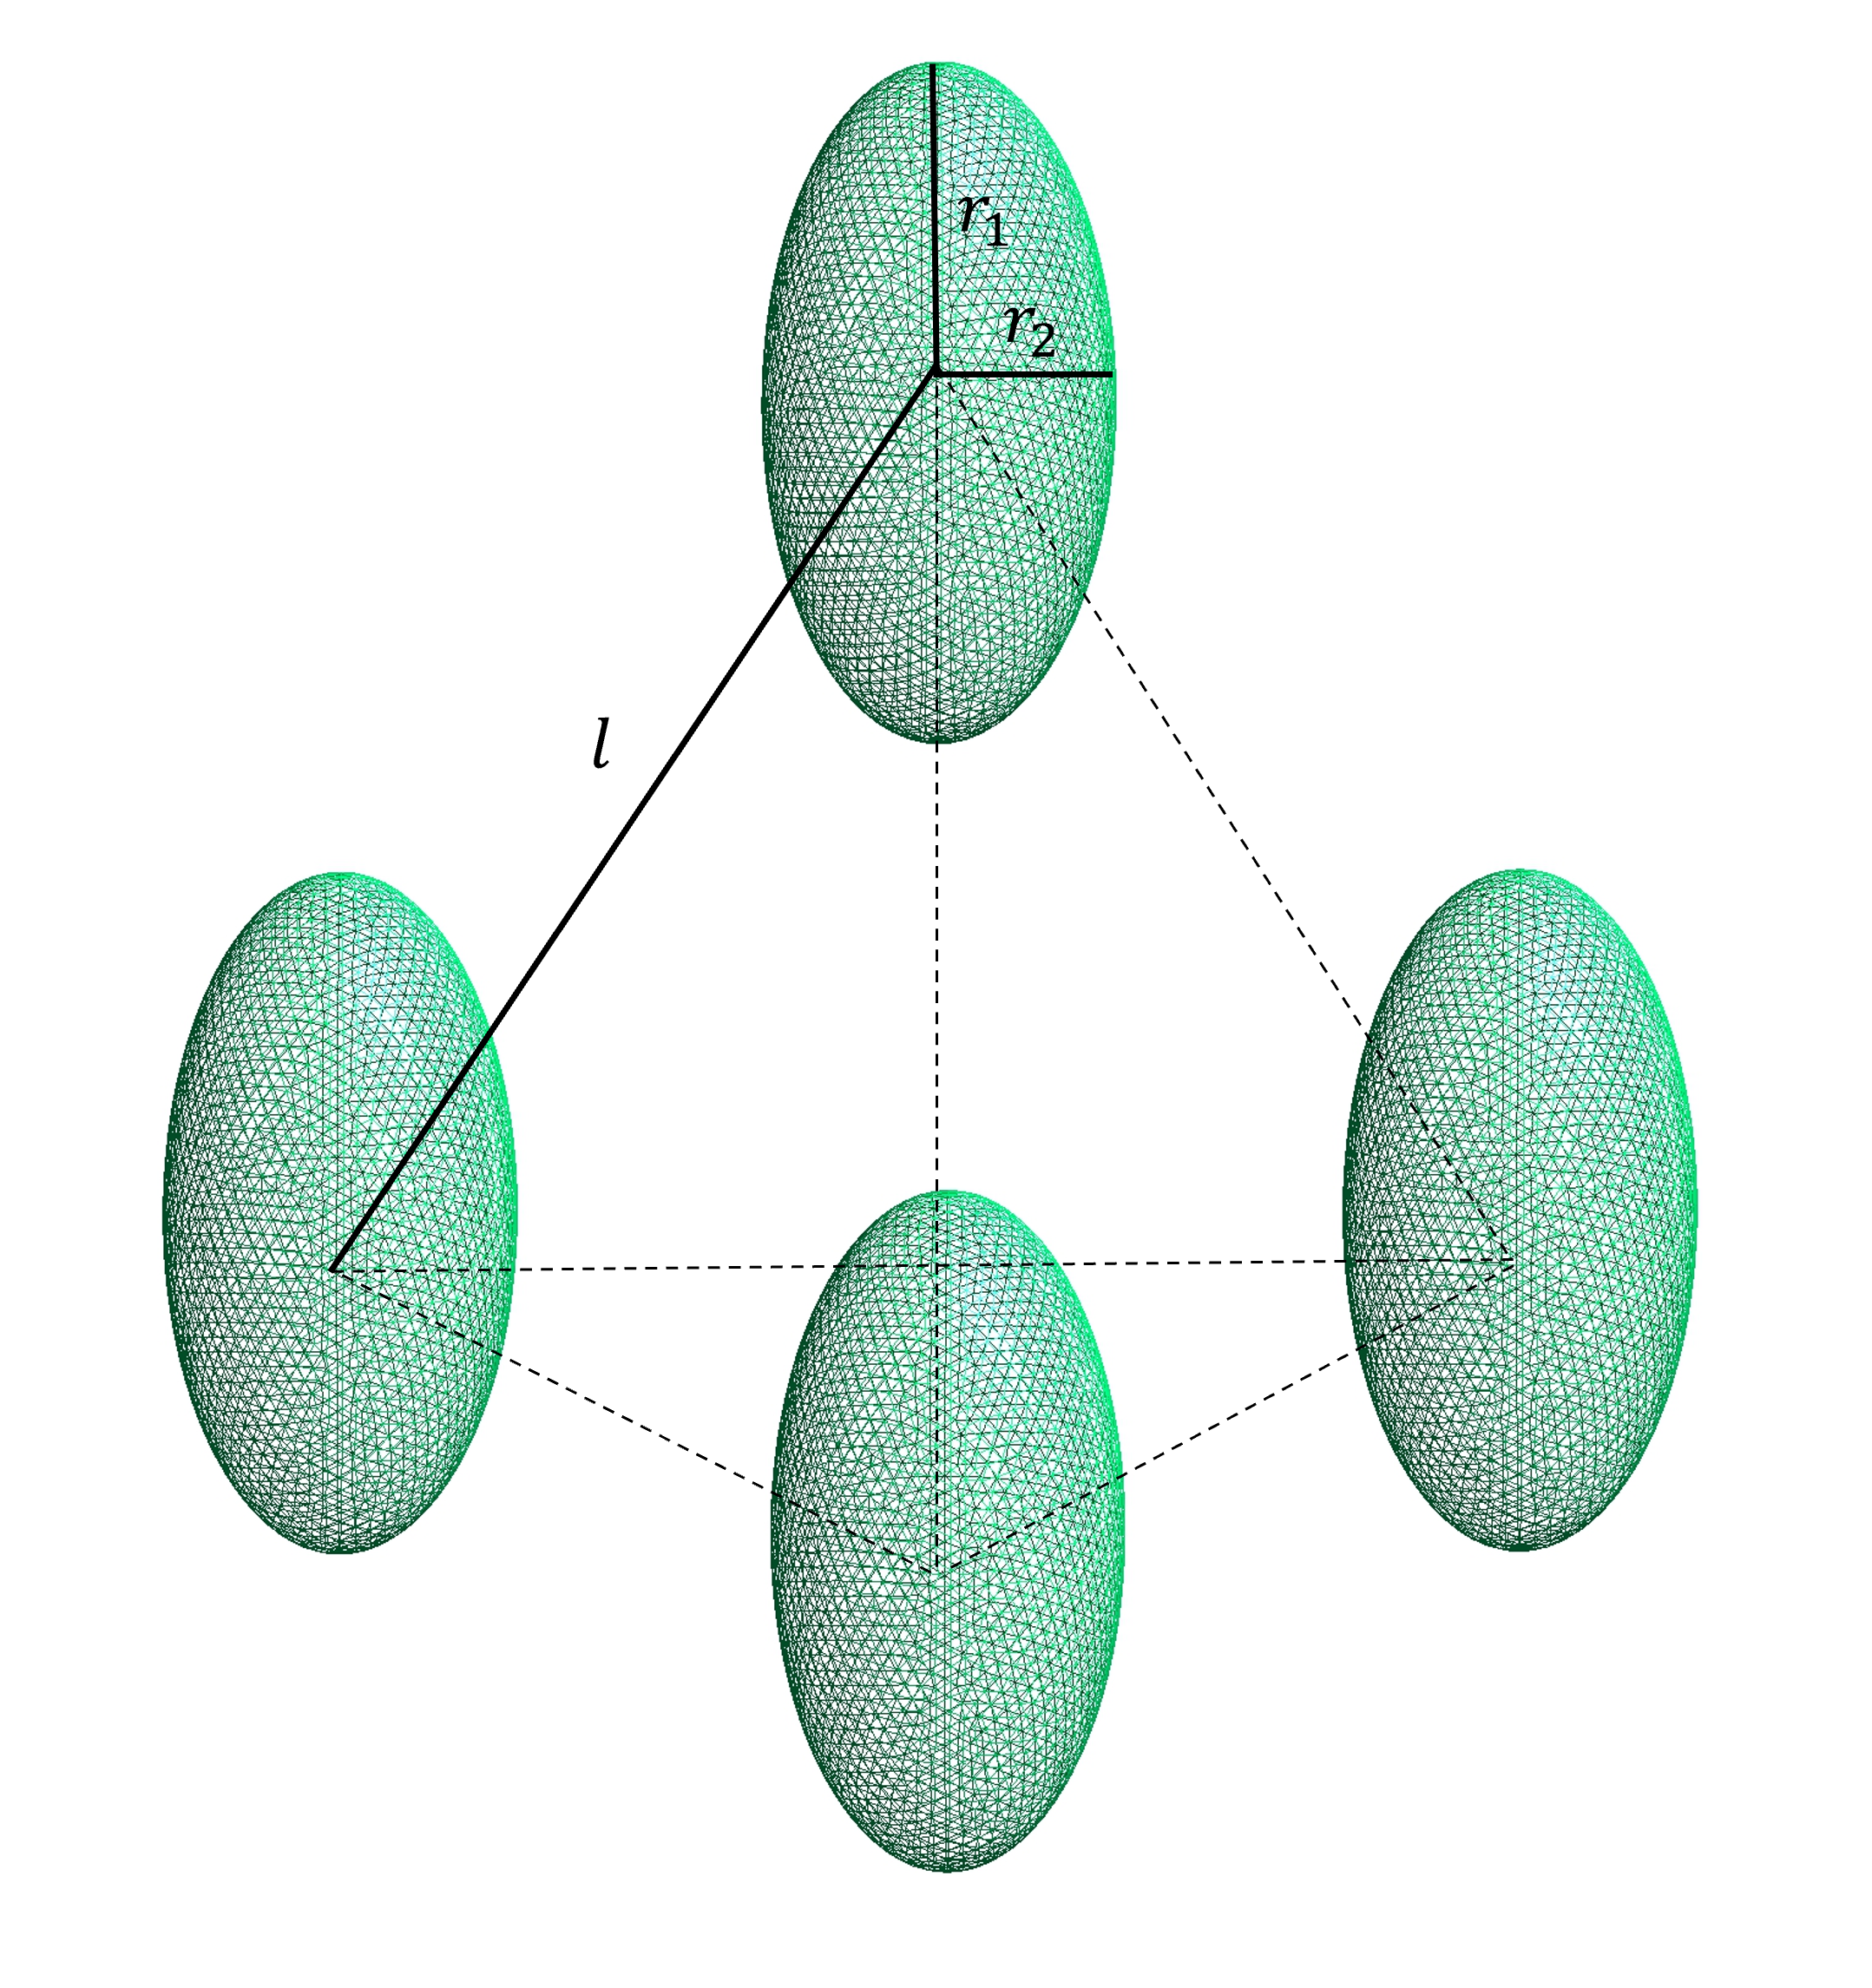
\includegraphics[scale = 0.4]{figures/4_ellip}
        \caption{No rotation}
        \label{No rotation 4}
        \end{subfigure}\\[1ex]
    \begin{subfigure}{.5\linewidth}
    \centering
    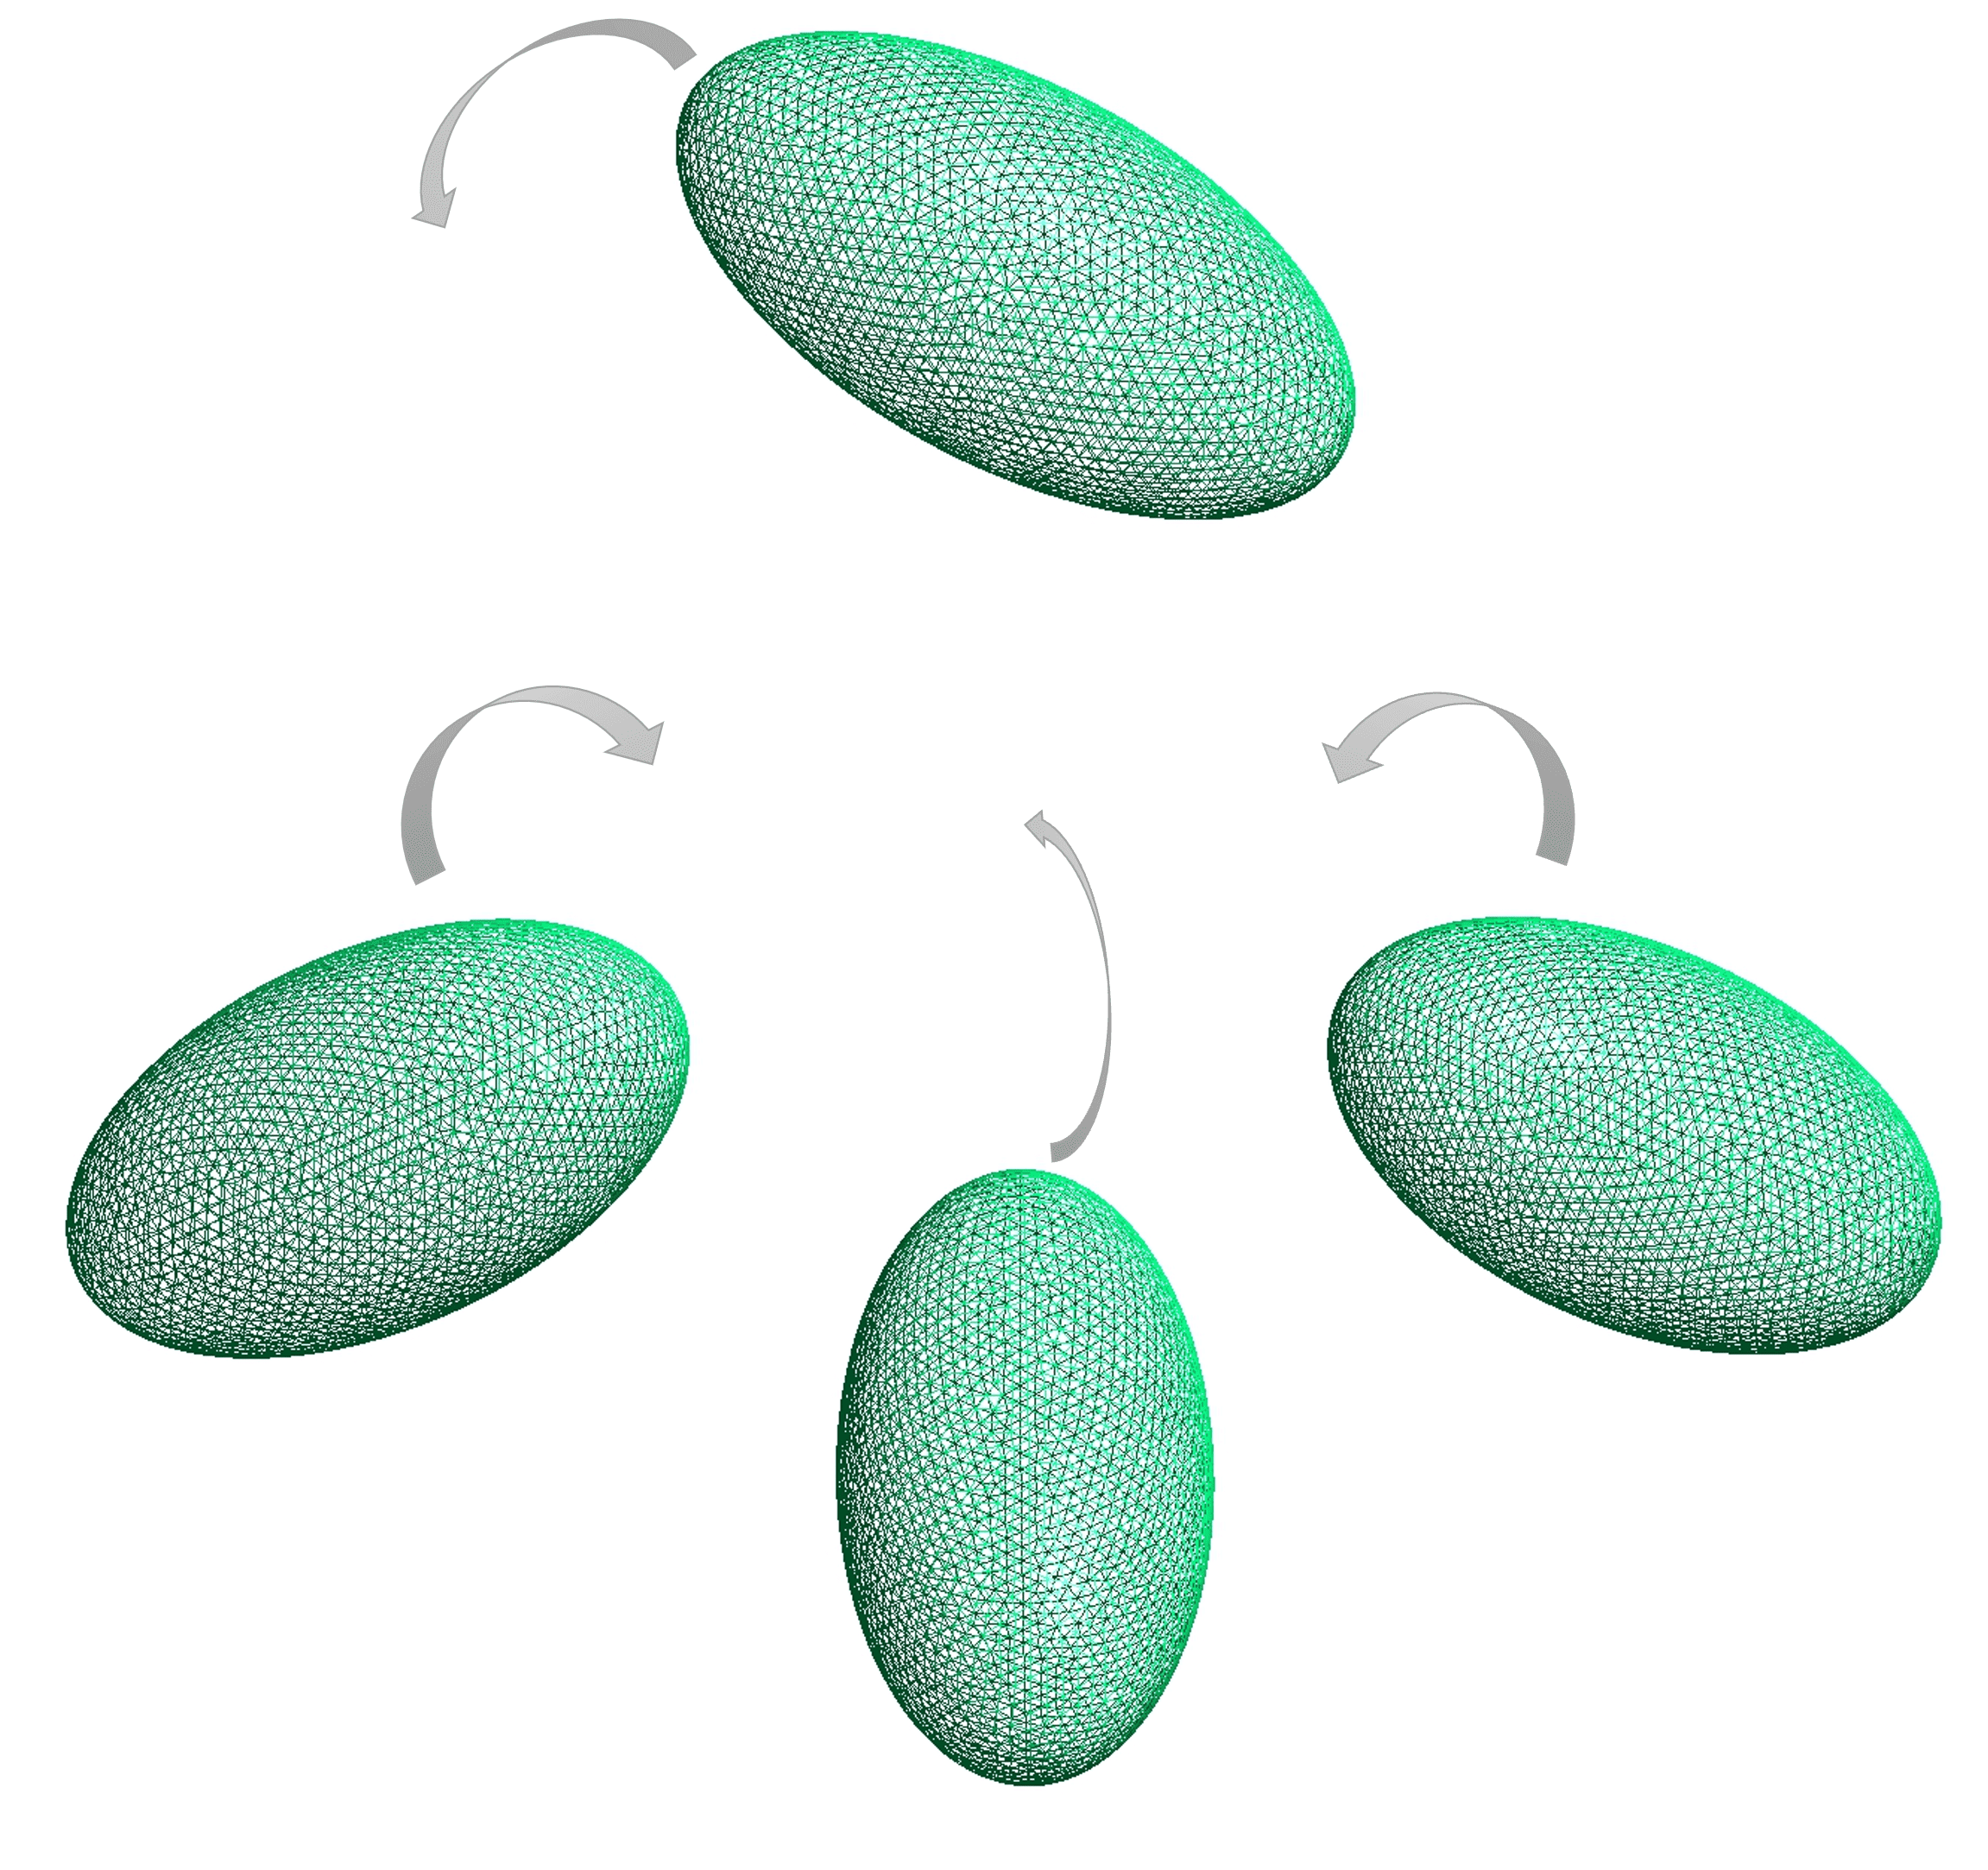
\includegraphics[scale = 0.09]{figures/4_ellip_in}
    \caption{Rotation inwards}
    \label{Rotation inwards 4}
    \end{subfigure}%
    \begin{subfigure}{.5\linewidth}
    \centering
    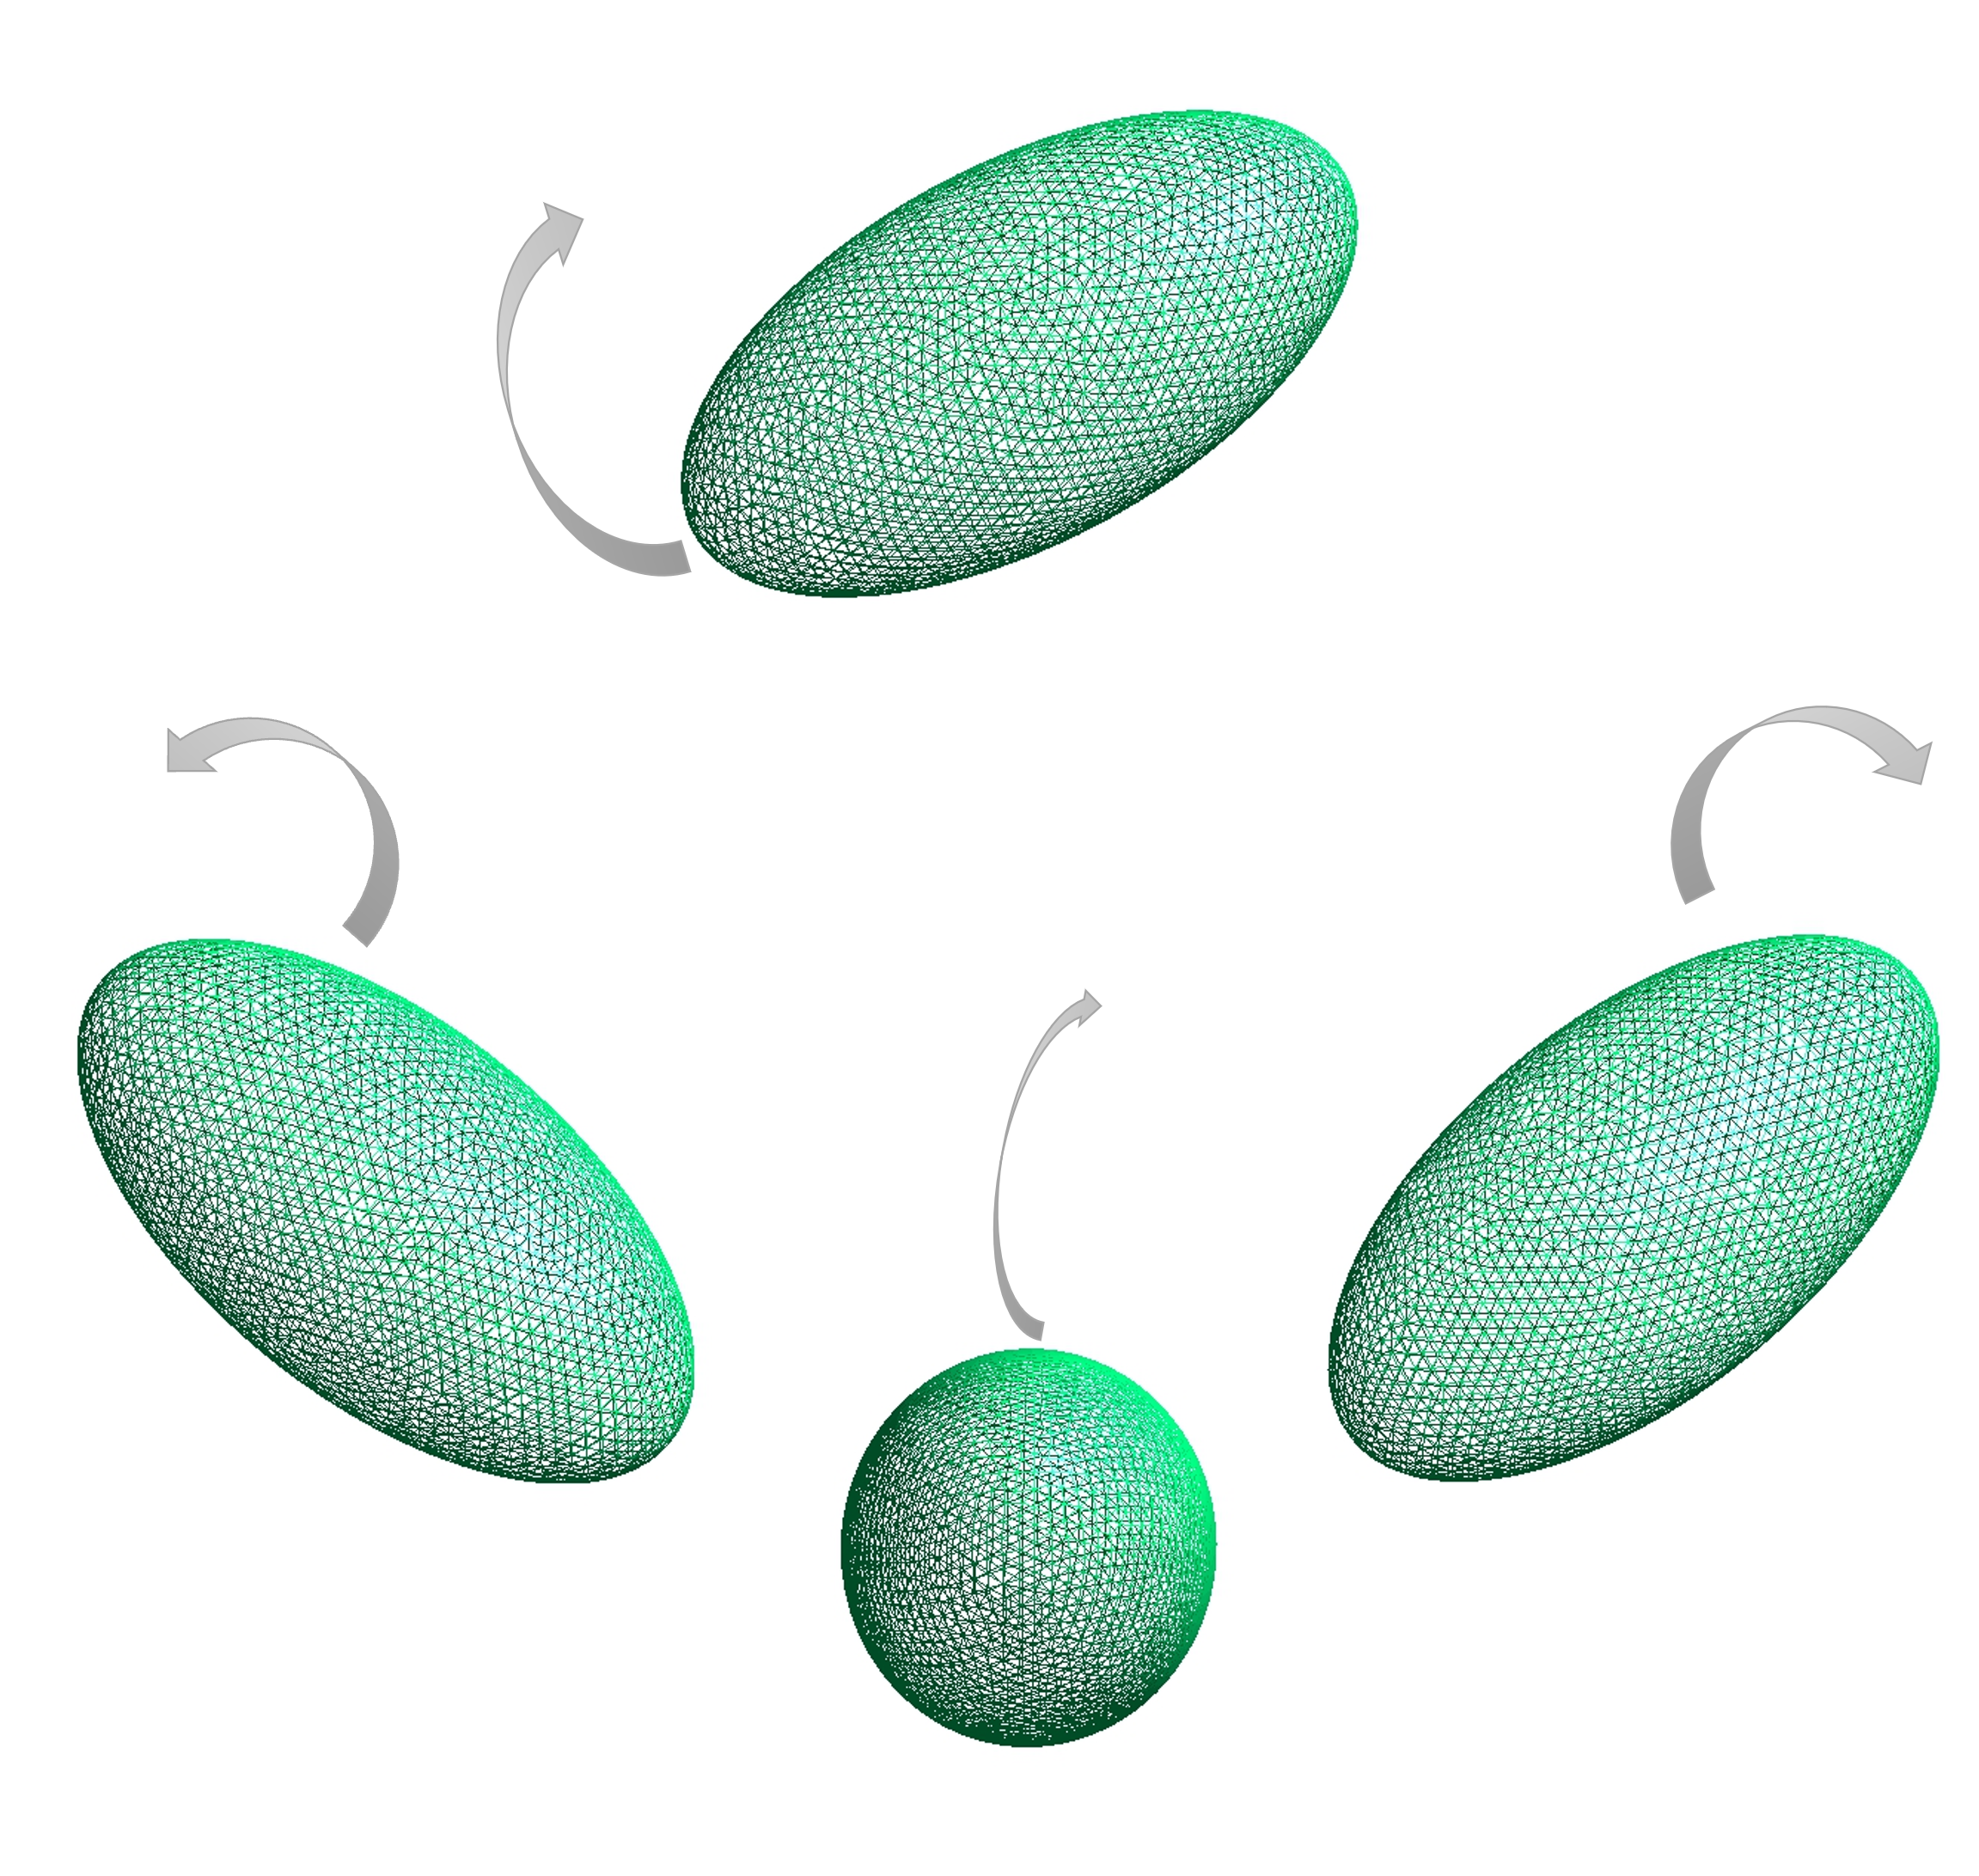
\includegraphics[scale = 0.4]{figures/4_ellip_out}
    \caption{Rotation outwards}
    \label{Rotation outwards 4}
    \end{subfigure}
    \caption{Four ellipsoids with or without rotations:  when $h_\text{fine}$ = 0.03, $\text{dim}(\mathsf{V}_{\mathrm{i}k}) = 11024$; 
    $h_\text{coarse}$ = 0.05, $\text{dim}(\mathsf{V}_{\mathrm{i}k}) = 4160$. The principal semi-axes of these ellipsoids are $r_{1} = 0.6$ and $r_{2} = 0.3$
    and they locate on the vertices of a regular octahedron with edge length $l = 2$.}
    \label{Four ellipsoids with or without rotations}
    \end{figure}

    \begin{figure}[H]
        \centering
        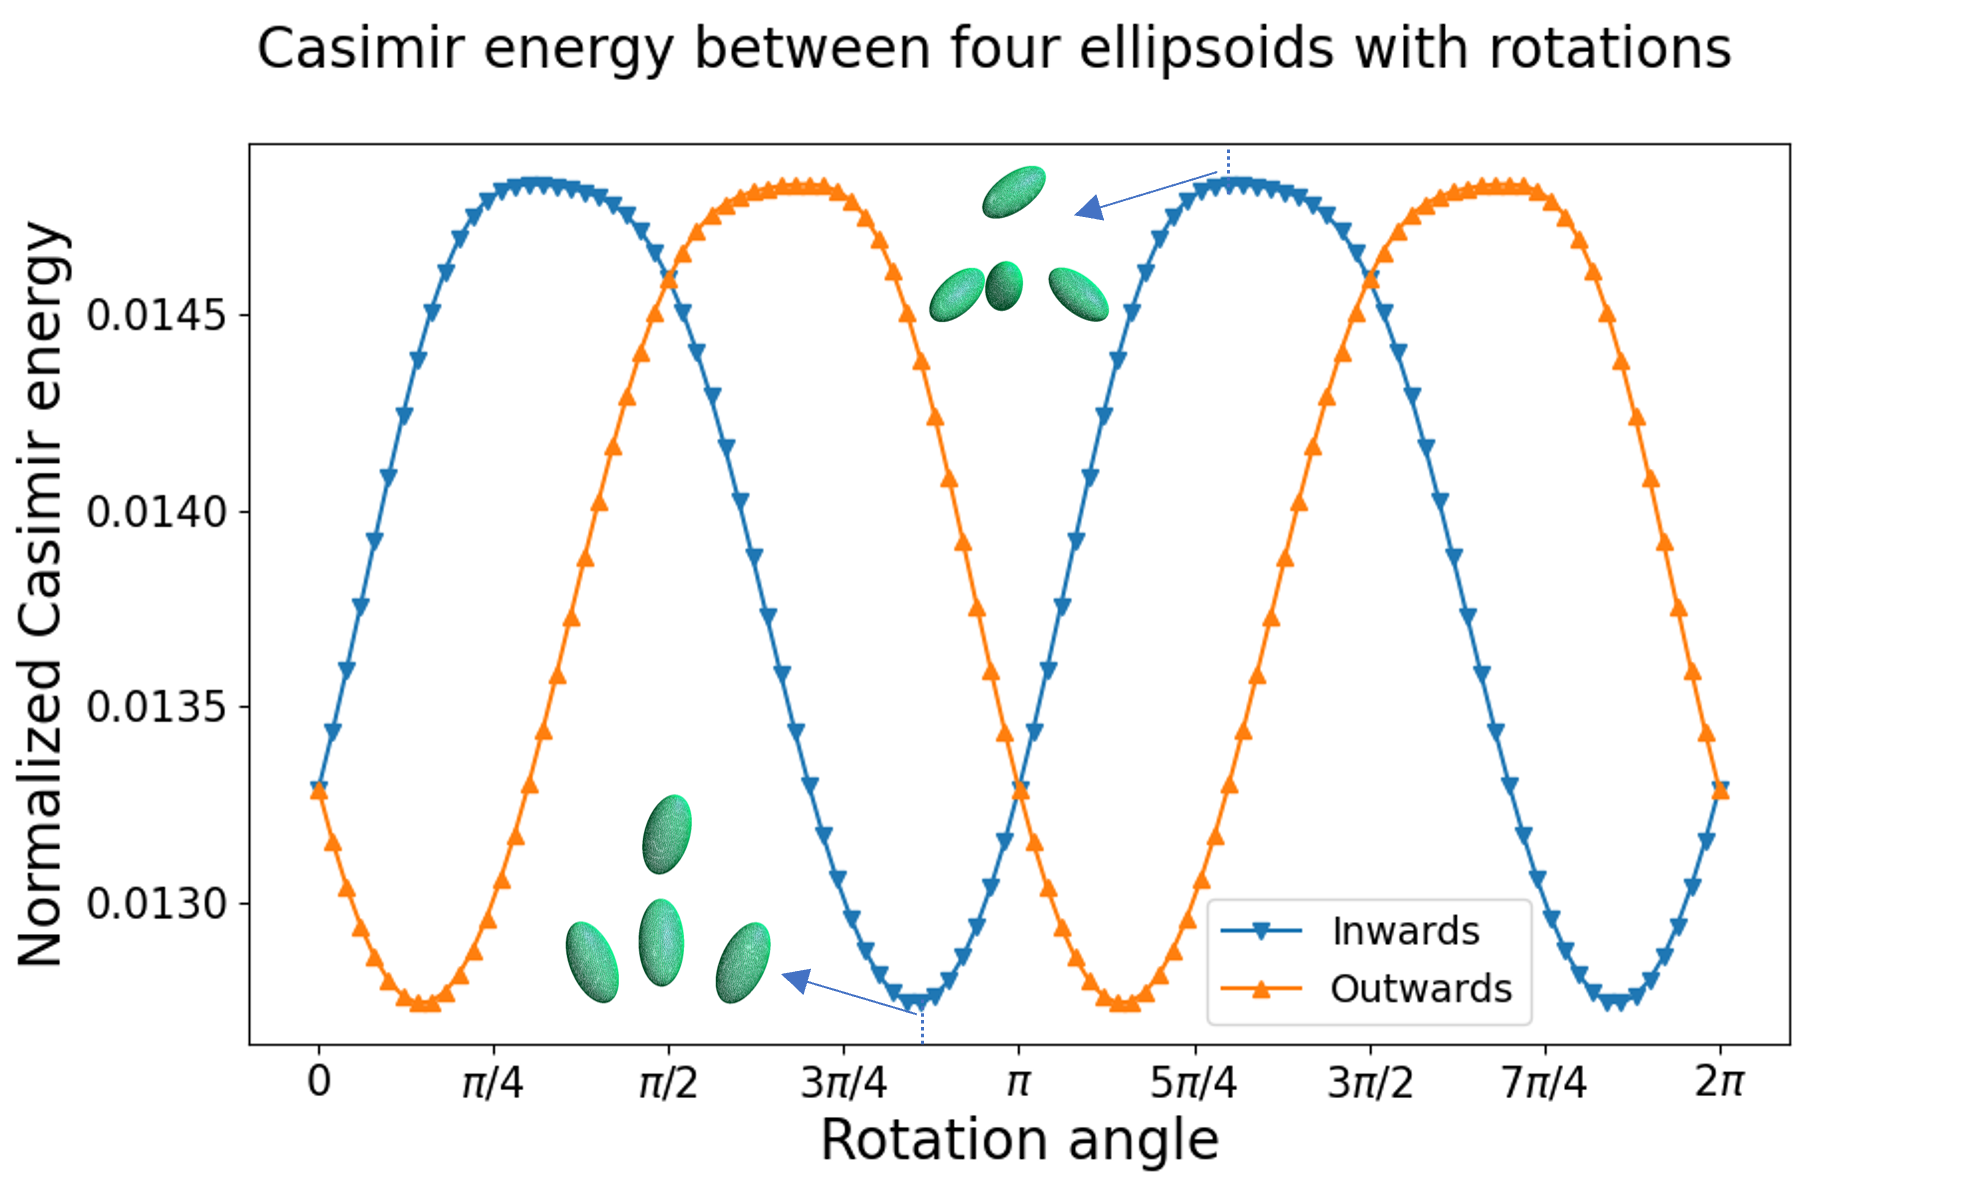
\includegraphics[scale = 1]{figures/CasE_4_ellip.png}
        \caption{The dependence of the Casimir energy and rotation angle of one of the ellipsoids. Inwards towards the centroid case (solid blue square).
        Outwards towards the centroid case (solid orange triangle).}
        \label{Four ellipsoids}
    \end{figure}

  The scatterers of the last example are described inside the Figure \ref{Six ellipsoids with or without rotations}. These six ellipsoids locate on the 
  vertices of a regular octahedron with edge length $l = 2$ and again the principal semi-axes of all these ellipsoids are $r_{1} = 0.6$ and $r_{2} = 0.3$ (shown 
  in the Figure \ref{Six ellipsoids with or without rotations}). This time, the ellipsoids rotate inwards and outwards 360 degrees towards the centroid of 
  this octahedron (Figure \ref{Rotation inwards 6} and Figure \ref{Rotation outwards 6}). By closely looking at these two rotation figures, we can notice that 
  Figure \ref{Rotation inwards 6} can be obtained by rotating Figure \ref{Rotation outwards 6} 180 degrees. Therefore, the Casimir energies for the inwards and 
  outwards cases are the same. Figure \eqref{Six ellipsoids} shows how the Casimir energy changes among these six ellipsoids as they rotate. 

\begin{figure}[H]
    \begin{subfigure}{\linewidth}
        \centering
        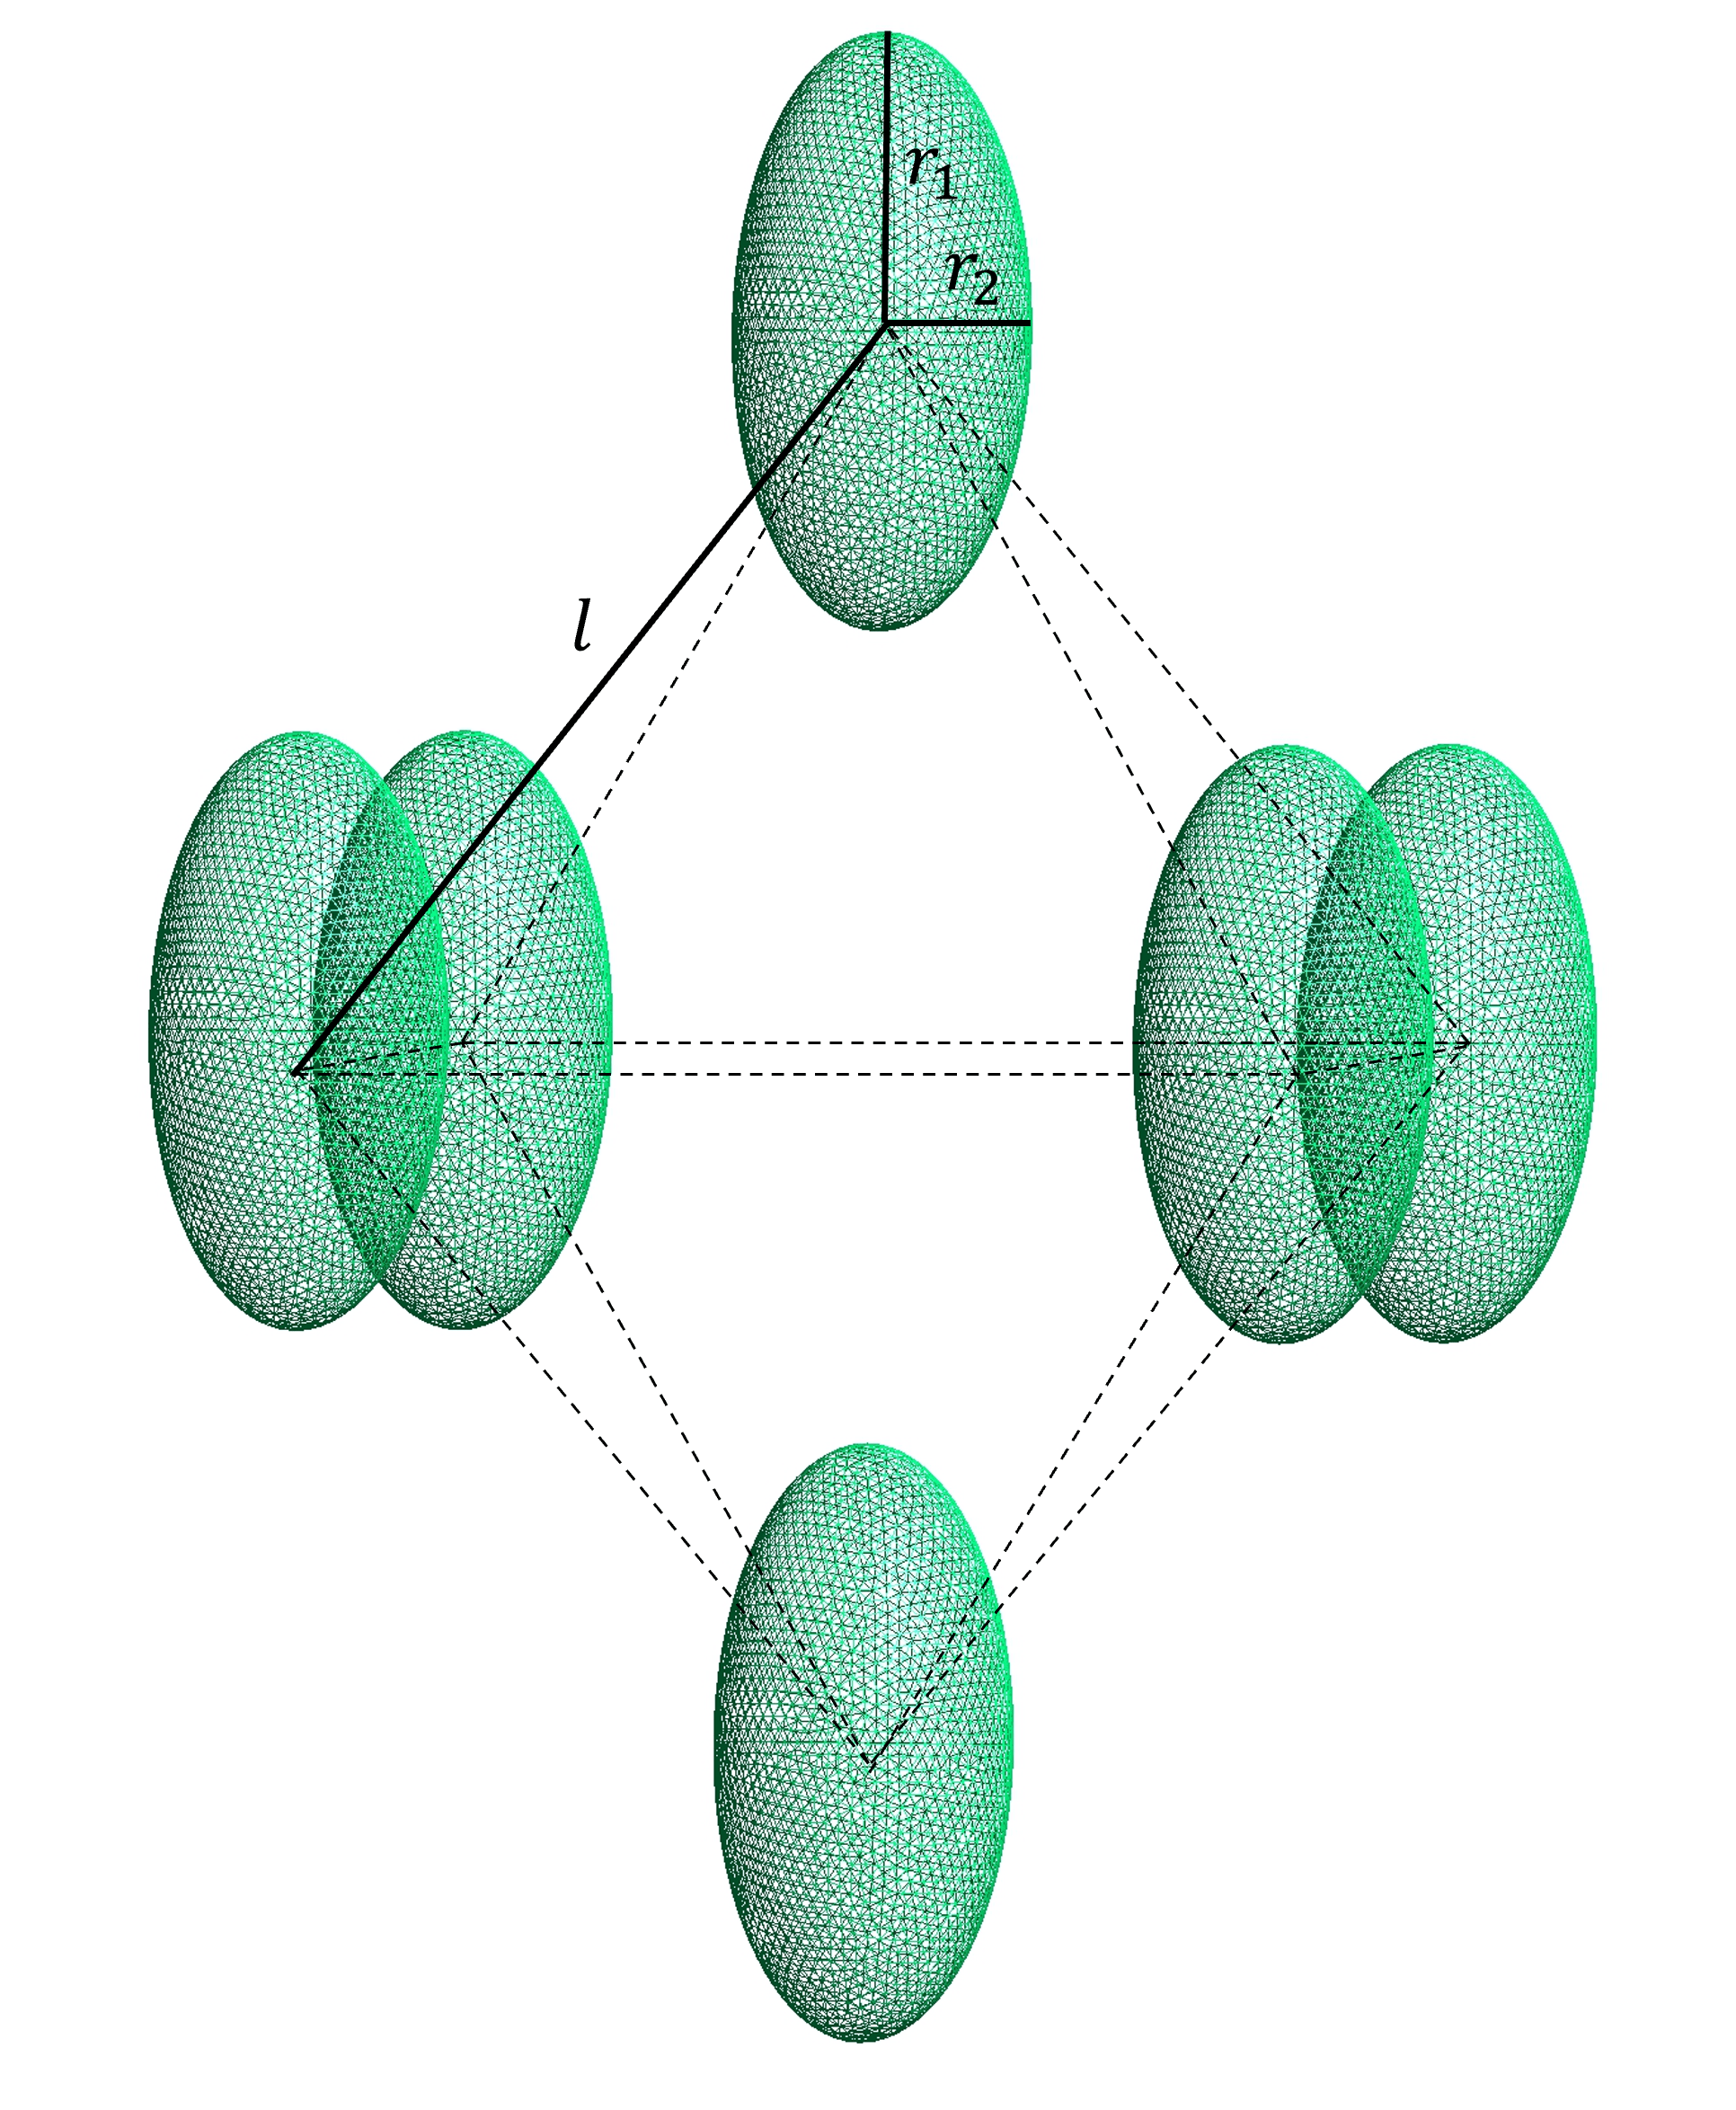
\includegraphics[scale = 0.4]{figures/6_ellip}
        \caption{No rotation}
        \label{No rotation 6}
        \end{subfigure}\\[1ex]
    \begin{subfigure}{.5\linewidth}
    \centering
    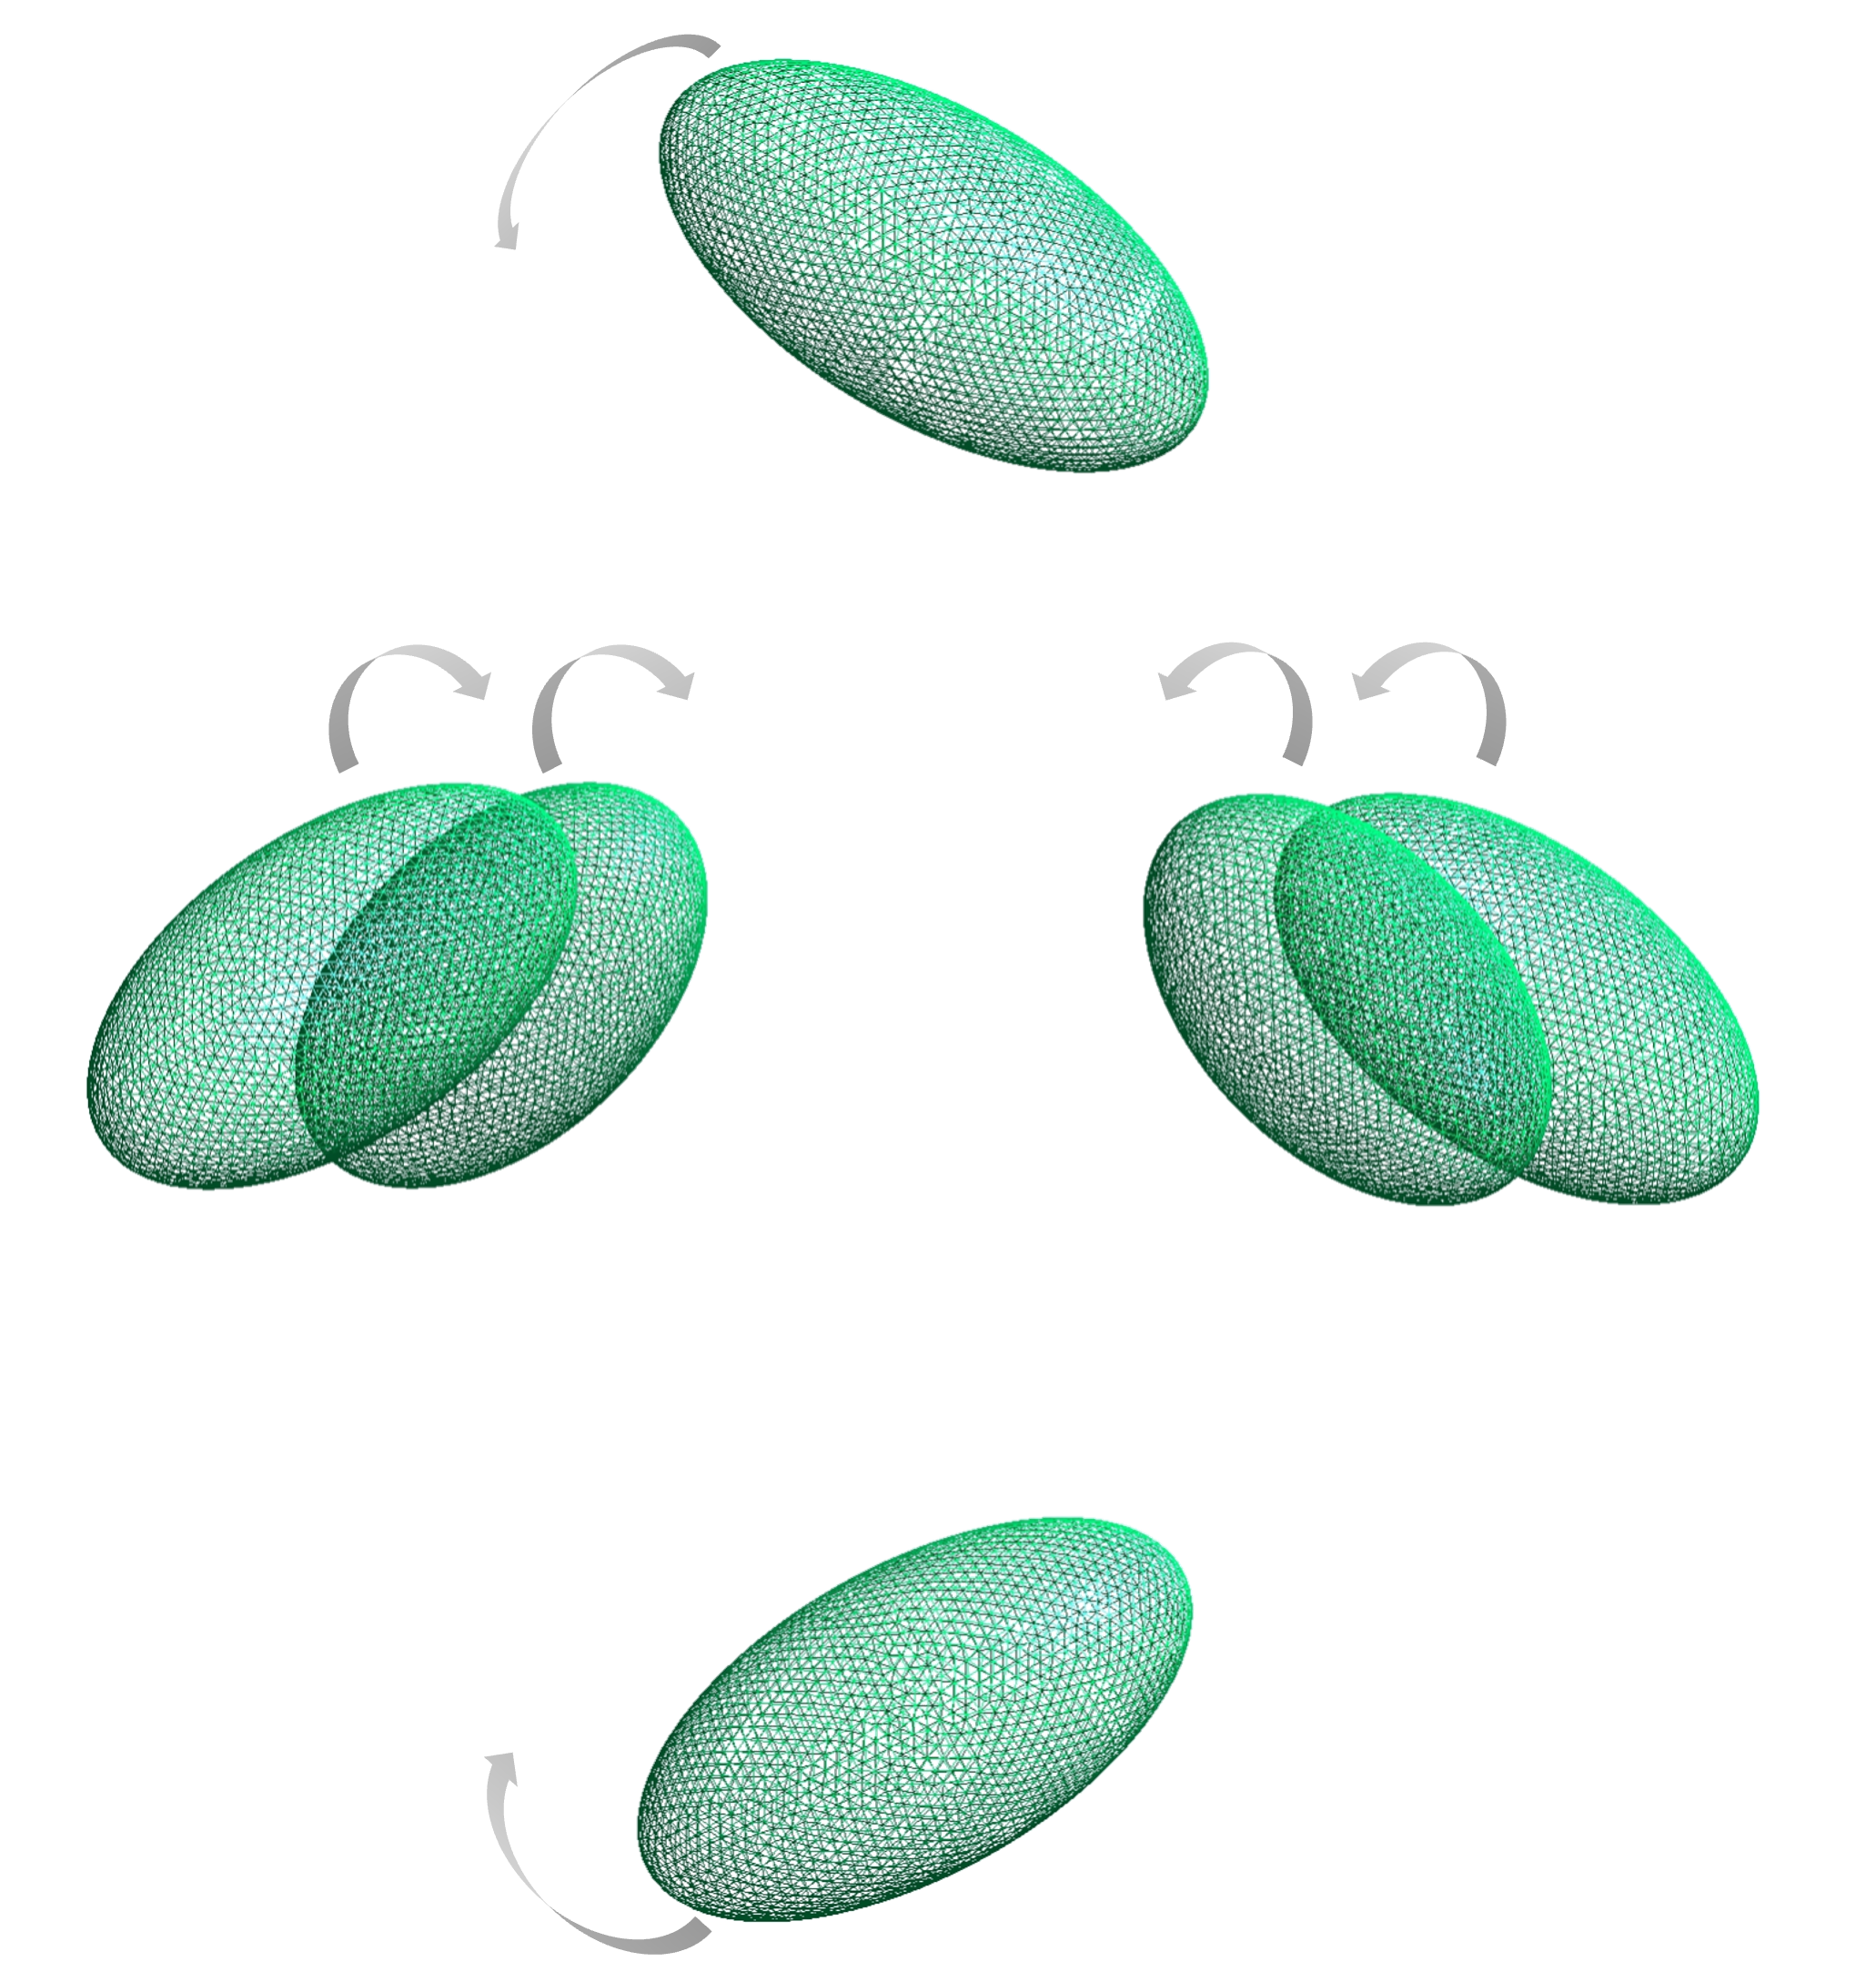
\includegraphics[scale = 0.4]{figures/6_ellip_in}
    \caption{Rotation inwards}
    \label{Rotation inwards 6}
    \end{subfigure}%
    \begin{subfigure}{.5\linewidth}
    \centering
    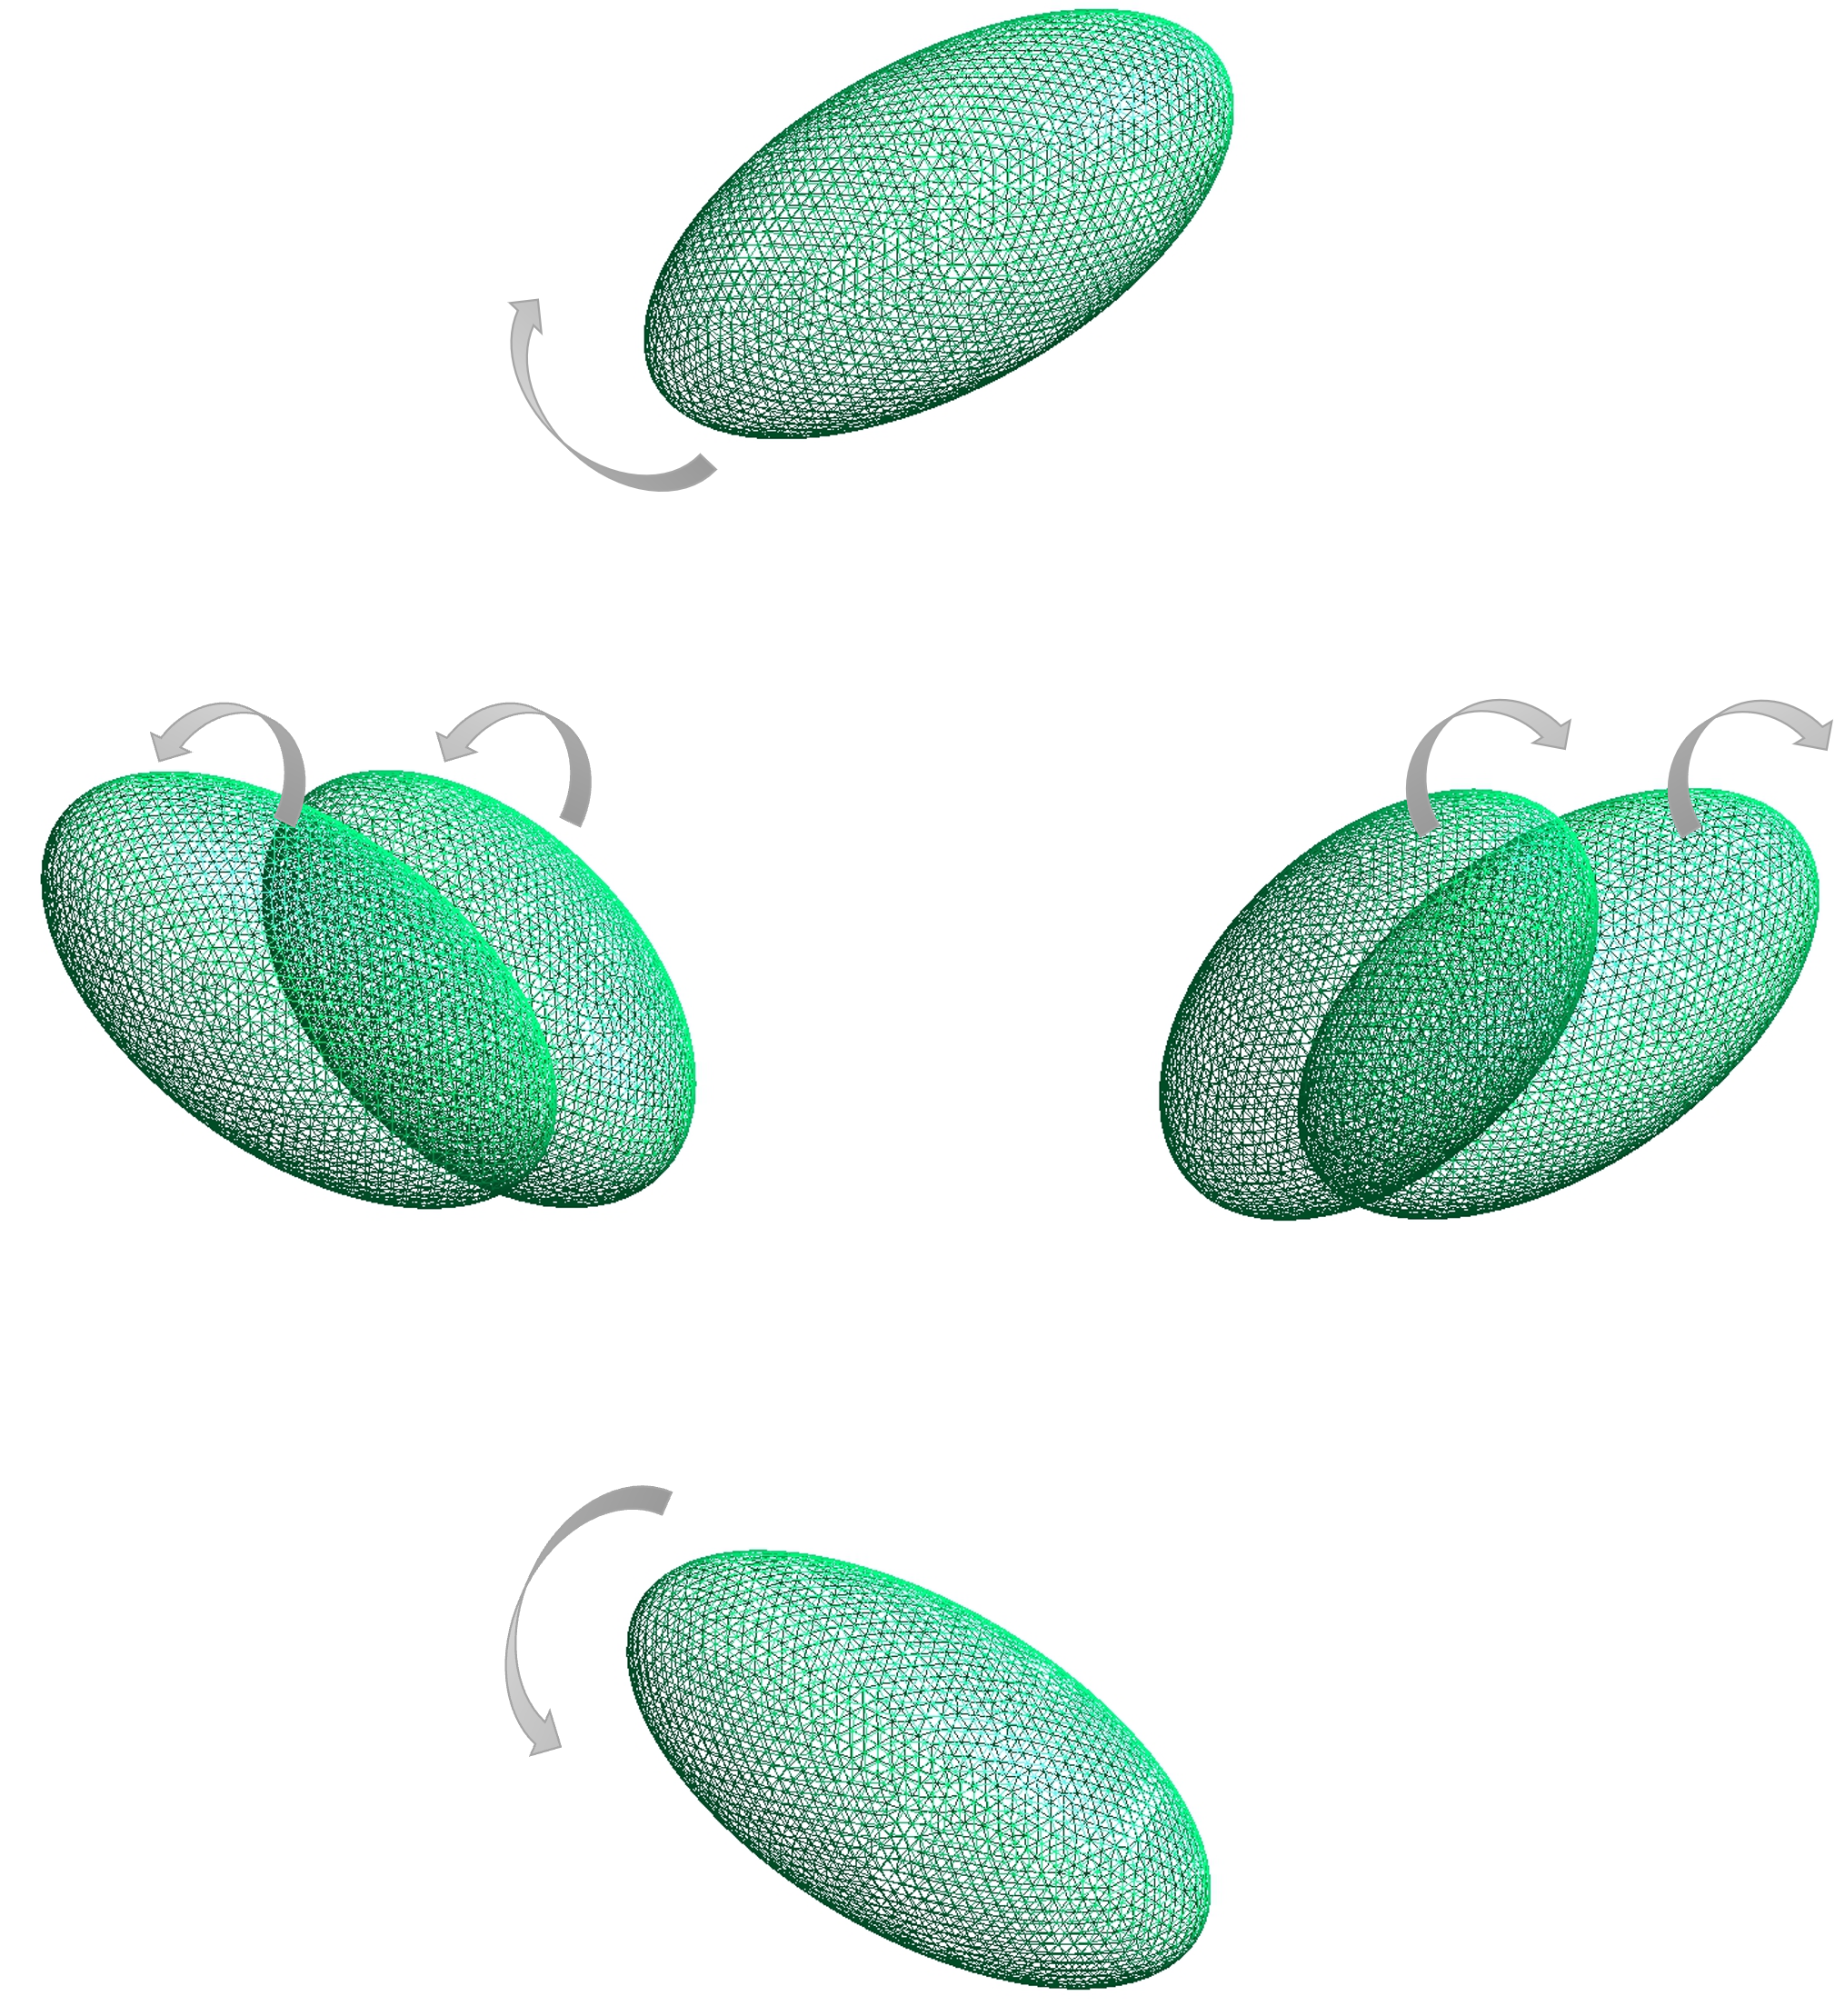
\includegraphics[scale = 0.4]{figures/6_ellip_out}
    \caption{Rotation outwards}
    \label{Rotation outwards 6}
    \end{subfigure}
    \caption{Six ellipsoids with or without rotations: when $h_\text{fine}$ = 0.03, $\text{dim}(\mathsf{V}_{\mathrm{i}k}) = 16536$;  $h_\text{coarse}$ = 0.05, $\text{dim}(\mathsf{V}_{\mathrm{i}k}) = 6240$.
    The principal semi-axes of these ellipsoids are $r_{1} = 0.6$ and $r_{2} = 0.3$
    and they locate on the vertices of a regular octahedron with edge length $l = 2$.}
    \label{Six ellipsoids with or without rotations}
    \end{figure}

    \begin{figure}[H]
        \centering
        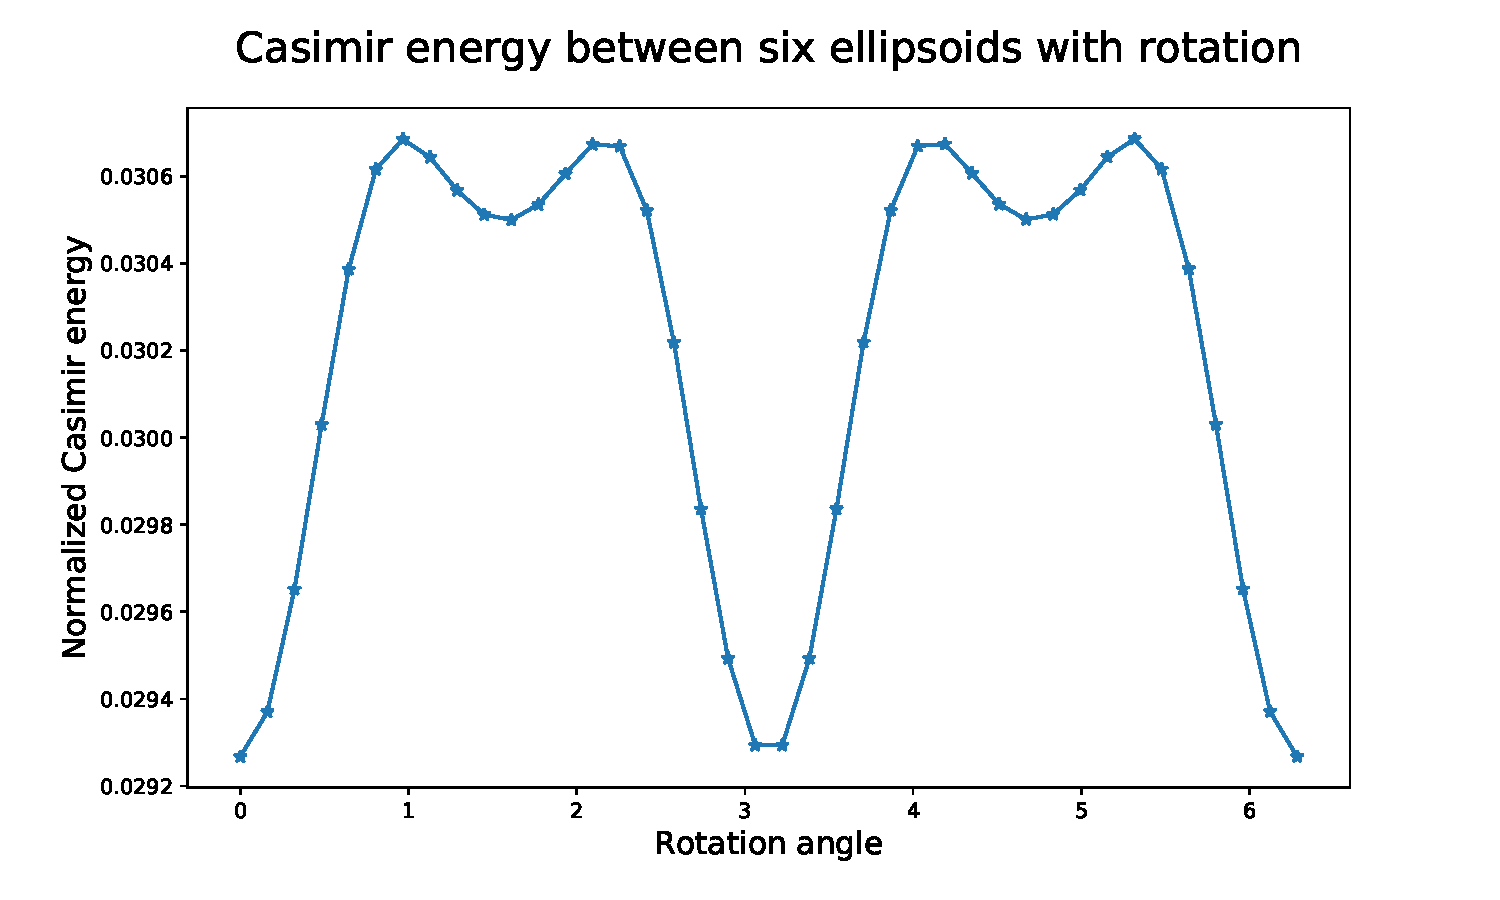
\includegraphics[scale = 0.5]{figures/CasE_6_ellip.pdf}
        \caption{The dependence of the Casimir energy and rotation angle of one of the ellipsoids.}
        \label{Six ellipsoids}
    \end{figure}